\documentclass[12pt,a4paper]{article}
\usepackage[utf8]{inputenc}
\usepackage[T1]{fontenc}
\usepackage{geometry}
\usepackage{graphicx}
\usepackage{float}
\usepackage{longtable}
\usepackage{booktabs}
\usepackage{array}
\usepackage{multirow}
\usepackage{wrapfig}
\usepackage{rotating}
\usepackage{listings}
\usepackage{color}
\usepackage{enumitem}
\usepackage{hyperref}
\usepackage{fancyhdr}
\usepackage{titlesec}
\usepackage{setspace}
\usepackage{parskip}
\usepackage[english]{babel}
\usepackage{subcaption}
\usepackage{url}
\setlength{\headheight}{15pt}
\addtolength{\topmargin}{-3pt}

% Page setup
\geometry{margin=1in}
\setlength{\parindent}{0pt}
\setlength{\parskip}{6pt}

% Header and footer
\pagestyle{fancy}
\fancyhf{}
\fancyhead[L]{\textbf{Vacation Management System - SRS}}
\fancyhead[R]{\thepage}
\renewcommand{\headrulewidth}{0.4pt}

% Title formatting
\titleformat{\section}{\Large\bfseries}{\thesection}{1em}{}
\titleformat{\subsection}{\large\bfseries}{\thesubsection}{1em}{}
\titleformat{\subsubsection}{\normalsize\bfseries}{\thesubsubsection}{1em}{}

% Custom colors
\definecolor{codegreen}{rgb}{0,0.6,0}
\definecolor{codegray}{rgb}{0.5,0.5,0.5}
\definecolor{codepurple}{rgb}{0.58,0,0.82}
\definecolor{backcolour}{rgb}{0.95,0.95,0.92}

% Code listing style
\lstdefinestyle{mystyle}{
    backgroundcolor=\color{backcolour},   
    commentstyle=\color{codegreen},
    keywordstyle=\color{magenta},
    numberstyle=\tiny\color{codegray},
    stringstyle=\color{codepurple},
    basicstyle=\ttfamily\footnotesize,
    breakatwhitespace=false,         
    breaklines=true,                 
    captionpos=b,                    
    keepspaces=true,                 
    numbers=left,                    
    numbersep=5pt,                  
    showspaces=false,                
    showstringspaces=false,
    showtabs=false,                  
    tabsize=2
}
\lstset{style=mystyle}

% Table style
\newcolumntype{P}[1]{>{\centering\arraybackslash}p{#1}}

\begin{document}

% Title Page
\begin{titlepage}
\centering
\vspace*{2cm}
{\Huge\bfseries Vacation Management System\par}
\vspace{1cm}
{\Large\bfseries Software Requirements Specification\par}
\vspace{2cm}
{\large Version 2.1\par}
\vspace{1cm}
{\large \today\par}
\vspace{2cm}
{\large Prepared for: Ejada\par}
\vspace{1cm}
{\large Prepared by: Omar Abdelrahman Abbas\par}
\vspace{1cm}
{\large Under supervision of: Ahmed Abdelwahab Mohamed\par}
\vspace{1cm}
{\large Document Type: Software Requirements Specification\par}
\vfill
\end{titlepage}

% Table of Contents
\tableofcontents
\newpage

% List of Figures
\listoffigures
\newpage

% List of Tables
\listoftables
\newpage

\section{Introduction}

\subsection{Purpose}
This Software Requirements Specification (SRS) document describes the functional and non-functional requirements for the Vacation Management System. The document serves as a comprehensive contract between the development team and stakeholders, providing a detailed understanding of what the system must accomplish based on the complete project scope and use cases.

\subsection{Scope}
The Vacation Management System is designed to automate the vacation request, approval, and cancellation processes while providing robust reporting capabilities for efficient vacation management. The system addresses inefficiencies in the current paper-based system, such as processing delays and inaccurate balance tracking due to manual errors and duplicate records.

The system scope includes:
\begin{itemize}
    \item Employee vacation request submission and management
    \item Vacation cancellation request processing
    \item Multi-level approval workflow (Employee → Manager → HR → General Manager)
    \item Vacation inquiry and search functionality
    \item Report generation (Single Transaction and Comparative Annual Reports)
    \item Automated vacation balance management
    \item Notification system for all stakeholders
\end{itemize}

\subsection{Definitions, Acronyms, and Abbreviations}
\begin{itemize}
    \item \textbf{HR}: Human Resources
    \item \textbf{SRS}: Software Requirements Specification
    \item \textbf{UI}: User Interface
    \item \textbf{PDF}: Portable Document Format
    \item \textbf{API}: Application Programming Interface
    \item \textbf{DB}: Database
    \item \textbf{UC}: Use Case
    \item \textbf{GM}: General Manager
    \item \textbf{ERD}: Entity Relationship Diagram
\end{itemize}

\subsection{References}
\begin{itemize}
    \item Project Scope Document
    \item All-UseCases.json - Complete Use Case Specifications
    \item Wireframe Specifications (All Screen Designs)
    \item Data Dictionary Documentation (Master and Screen-level)
    \item System Diagrams (Context, State, Workflow)
\end{itemize}

\subsection{Overview}
The remainder of this document is organized as follows:
\begin{itemize}
    \item Section 2: Overall Description
    \item Section 3: System Architecture and Context
    \item Section 4: Business Rules and Logic
    \item Section 5: User Requirements / Use Cases
    \item Section 6: Functional Requirements
    \item Section 7: Non-Functional Requirements
    \item Section 8: User Interface Overview
    \item Section 9: Data Requirements Overview
    \item Section 10: System Messages
    \item Section 11: Appendices
    \item Section 12: Document Approval
\end{itemize}

\section{Overall Description}

\subsection{Product Perspective}
The Vacation Management System is a web-based application with mobile support that integrates with existing HR systems. It operates as a standalone module that can be deployed independently or integrated with larger enterprise systems.

\subsection{Product Functions}
The system provides the following core functionalities:

\begin{enumerate}
    \item \textbf{Vacation Request Management}
    \begin{itemize}
        \item Create vacation requests (Annual and Sick leave types)
        \item File attachment capabilities (mandatory for sick leave)
        \item Real-time validation and balance checking
        \item No modification capability after submission
    \end{itemize}
    
    \item \textbf{Vacation Cancellation Management}
    \begin{itemize}
        \item Cancel pending or approved requests before start date
        \item Cancellation reason tracking
        \item Approval workflow for cancellations
    \end{itemize}
    
    \item \textbf{Approval Workflow}
    \begin{itemize}
        \item Multi-level approval process (Employee → Manager → HR → GM)
        \item Automatic escalation after 2 days of delay
        \item Manager and HR review capabilities
    \end{itemize}
    
    \item \textbf{Reporting and Analytics}
    \begin{itemize}
        \item Single transaction reports (PDF)
        \item Comparative annual reports by department
        \item Department-wise vacation analytics
    \end{itemize}
    
    \item \textbf{Inquiry and Search}
    \begin{itemize}
        \item Advanced search capabilities with multiple filters
        \item Export functionality to Excel
        \item Pagination and result management
    \end{itemize}
    
    \item \textbf{Automated Balance Management}
    \begin{itemize}
        \item Automatic vacation balance calculation
        \item Entitlement rules (21/30 days based on service/age)
        \item No manual overrides permitted
    \end{itemize}
    
    \item \textbf{Notification System}
    \begin{itemize}
        \item Real-time notifications for all stakeholders
        \item Context-aware notification types
        \item Quick navigation to related screens
    \end{itemize}
\end{enumerate}

\subsection{User Classes and Characteristics}
\begin{table}[H]
\centering
\begin{tabular}{|p{3cm}|p{4cm}|p{4cm}|}
\hline
\textbf{User Class} & \textbf{Characteristics} & \textbf{Access Rights} \\
\hline
Employees & Full-time Muslim Saudi employees, non-trainees & Submit requests, view own requests, cancel requests \\
\hline
Direct Managers & Supervisors, approve subordinate requests & Review, approve/reject requests, view team reports \\
\hline
HR Personnel & Administrative users, manage policies & Full access, policy management, all reports \\
\hline
General Managers & Senior management, final approval & Final approval, all reports access, system oversight \\
\hline
System Administrators & Technical users, system maintenance & Full system access, configuration management \\
\hline
\end{tabular}
\caption{User Classes and Access Rights}
\end{table}

\subsection{Operating Environment}
\begin{itemize}
    \item \textbf{Platform}: Web-based application with mobile responsive design
    \item \textbf{Browsers}: Chrome, Firefox, Safari, Edge (latest versions)
    \item \textbf{Mobile}: iOS 12+, Android 8+
    \item \textbf{Database}: SQL Server/MySQL/PostgreSQL
    \item \textbf{Server}: Windows/Linux server environment
\end{itemize}

\subsection{Design and Implementation Constraints}
\begin{itemize}
    \item Compliance with Saudi vacation regulations
    \item Integration with existing HR systems
    \item Support for Arabic and English languages
    \item Mobile-first responsive design
    \item PDF generation capabilities
    \item Real-time notifications
    \item No modification of submitted requests
\end{itemize}

\subsection{Assumptions and Dependencies}
\begin{itemize}
    \item Existing employee database is available
    \item Network infrastructure supports web access
    \item Users have basic computer literacy
    \item HR policies are well-defined and documented
    \item Integration APIs are available for external systems
    \item All employees are full-time Muslim Saudi employees
\end{itemize}

\section{System Architecture and Context}

\subsection{System Context Diagram}
The Vacation Management System operates within a broader organizational context, interacting with various stakeholders and external systems. The following diagram shows how the system integrates with the broader organizational ecosystem:

\begin{figure}[H]
\centering
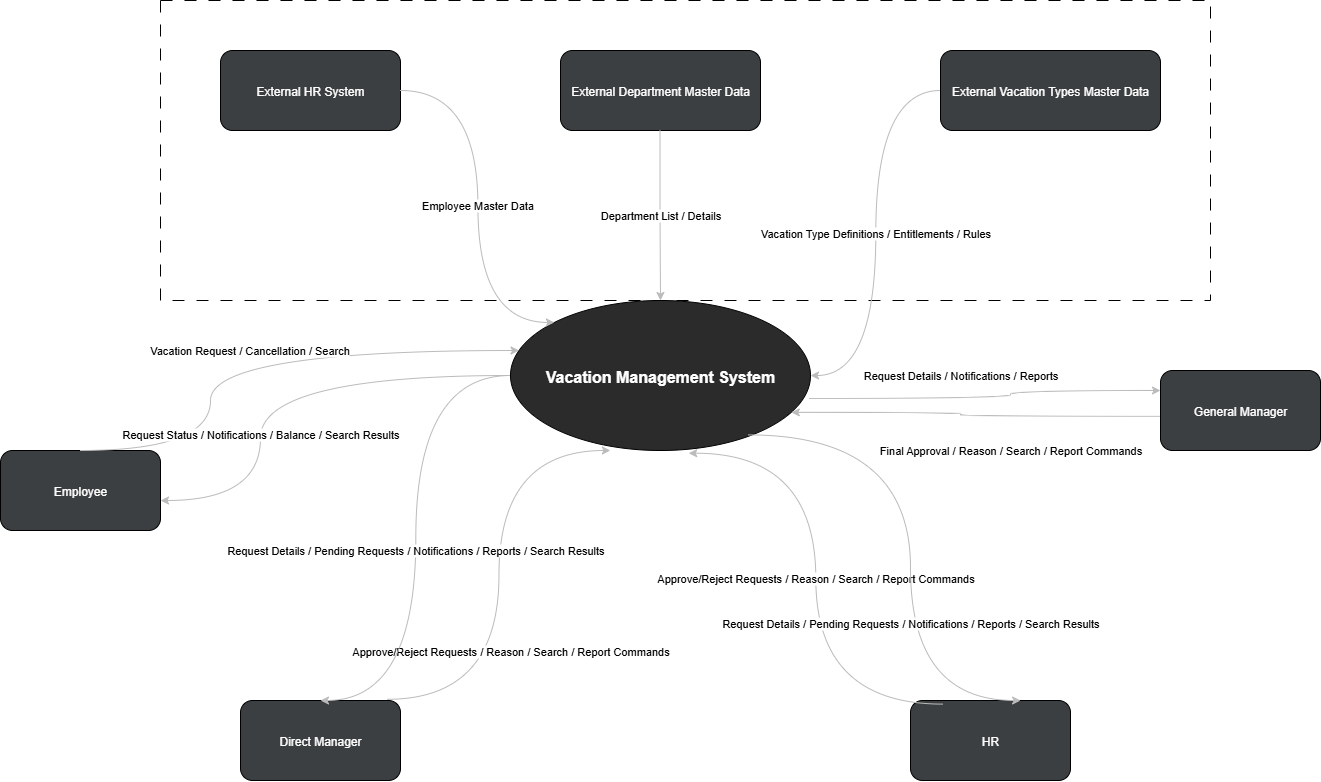
\includegraphics[width=0.9\textwidth]{Diagrams/Context/context.drawio.png}
\caption{System Context Diagram - Vacation Management System Integration}
\label{fig:context}
\end{figure}

\subsection{System Architecture Overview}
The system follows a three-tier architecture designed for scalability and maintainability:

\begin{itemize}
    \item \textbf{Presentation Tier}: Web and mobile interfaces with responsive design
    \item \textbf{Business Logic Tier}: Application services, workflows, and business rules engine
    \item \textbf{Data Tier}: Database, file storage, and integration services
\end{itemize}

\subsection{Core System Components}
The system is built around these key components:

\begin{itemize}
    \item \textbf{User Management Module}: Authentication, authorization, and role-based access control
    \item \textbf{Vacation Management Module}: Core business logic for request processing
    \item \textbf{Workflow Engine}: Multi-level approval process management with escalation
    \item \textbf{Reporting Module}: PDF generation and data export capabilities
    \item \textbf{Notification Module}: Real-time communication and alert system
    \item \textbf{Balance Management Module}: Automated vacation balance calculations
\end{itemize}

\subsection{System State Management}
The system manages various states for vacation requests and the overall workflow. The following state diagram illustrates the complete lifecycle of a vacation request:

\begin{figure}[H]
\centering
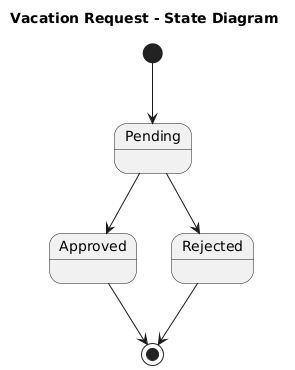
\includegraphics[width=0.6\textwidth]{Diagrams/State-Diagram/State-Diagram.png}
\caption{Vacation Request State Diagram - Complete Request Lifecycle}
\label{fig:state-diagram}
\end{figure}

\subsection{Core Workflow Processes}
The system implements several key workflow processes that define the approval and processing logic:

\subsubsection{Basic Vacation Request Flow}
The standard vacation request follows this workflow:

\begin{figure}[H]
\centering
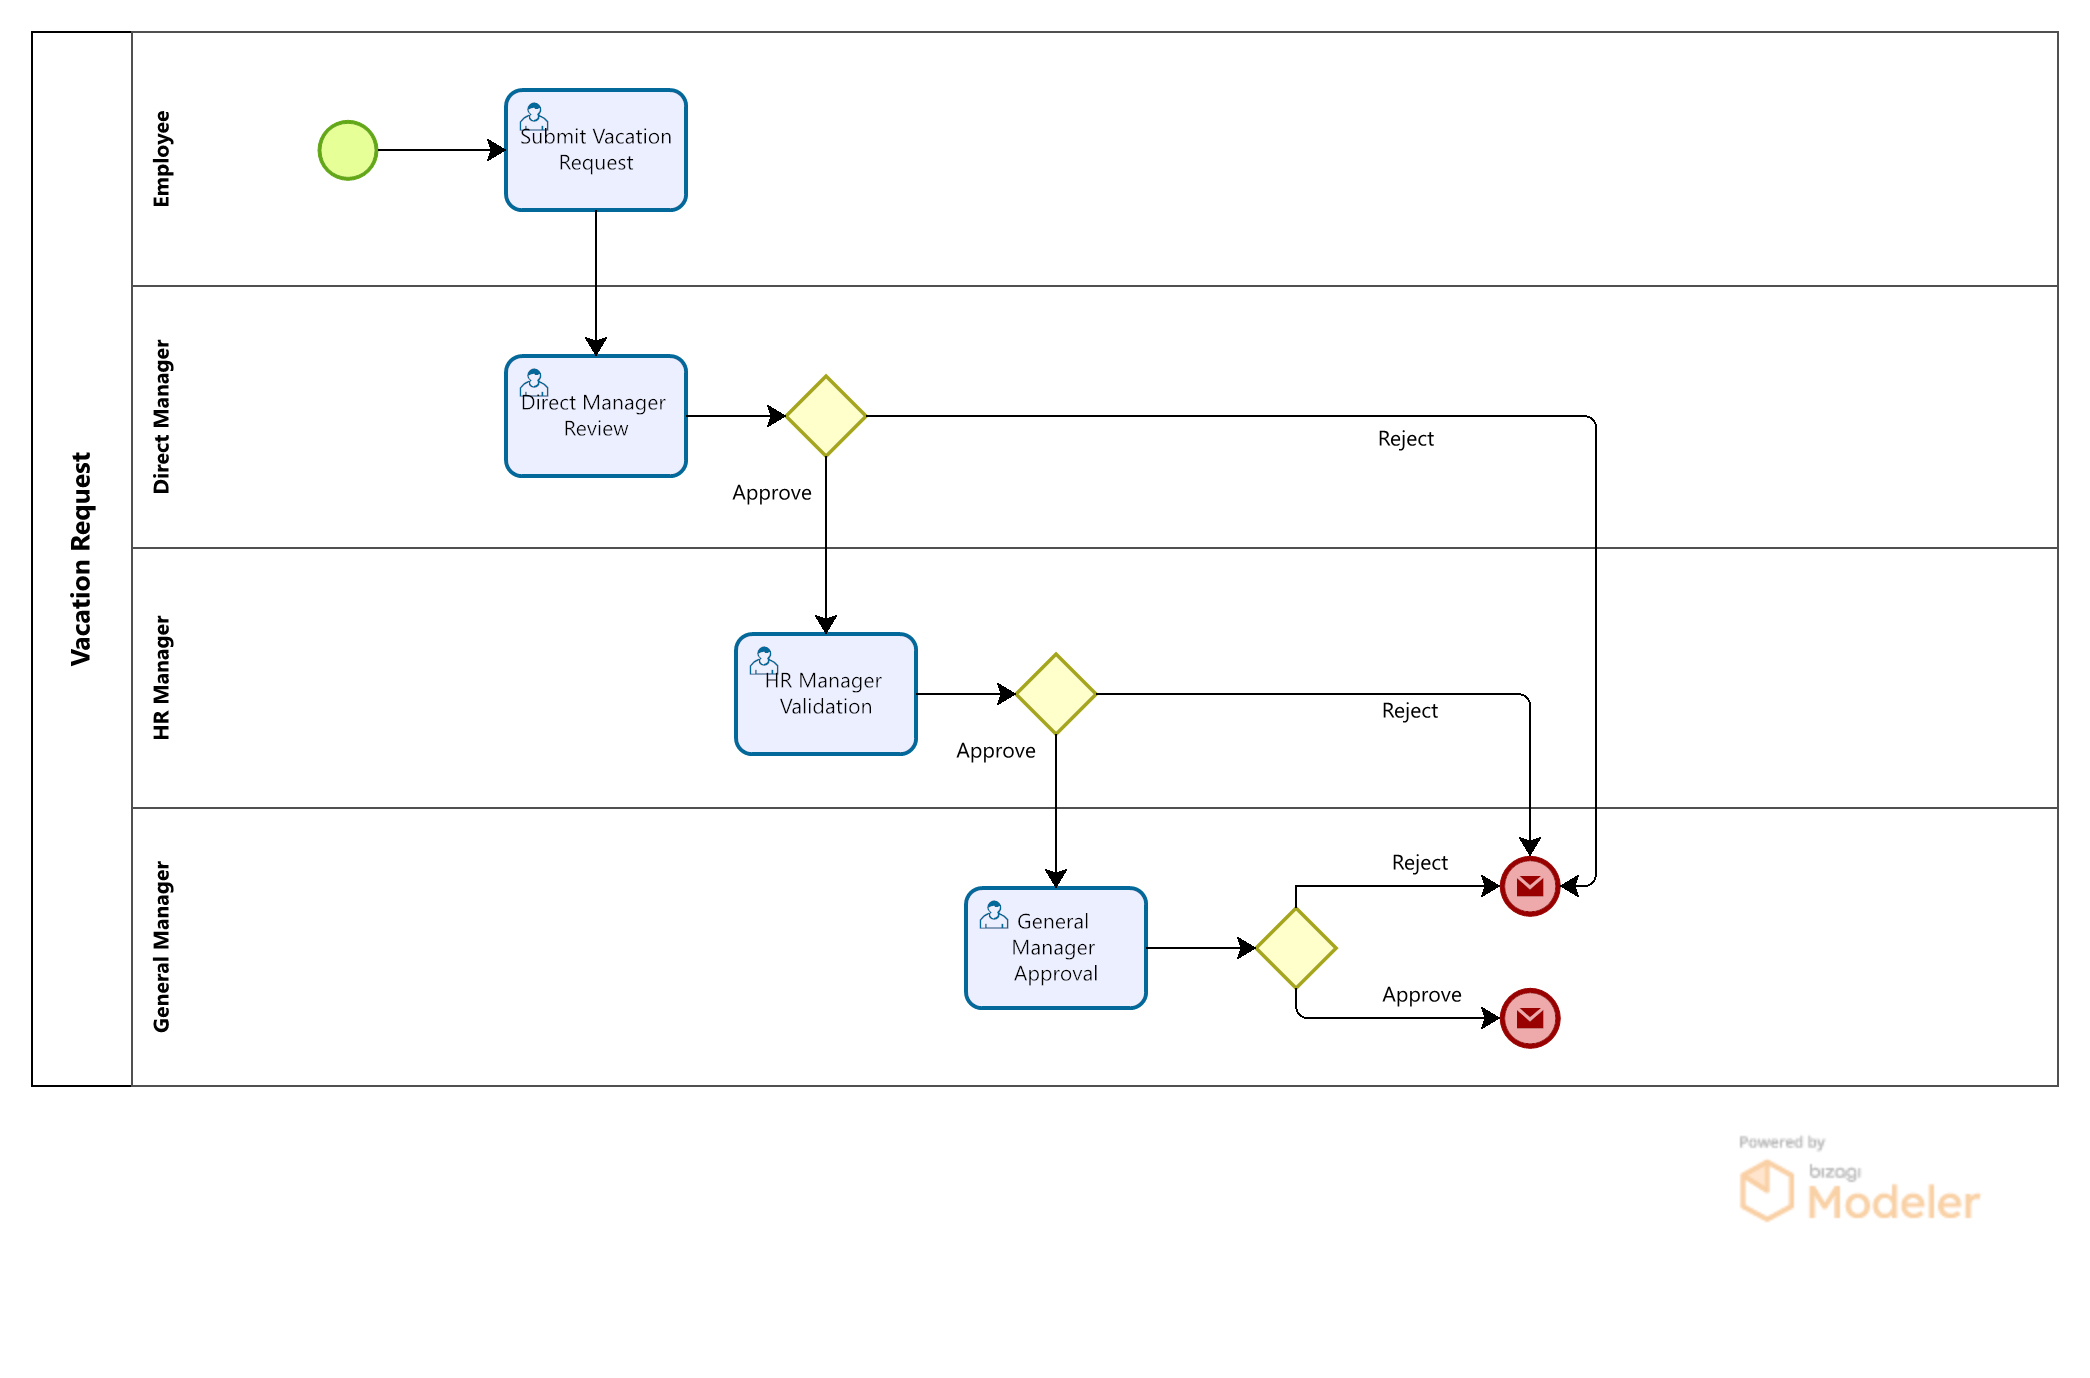
\includegraphics[width=0.9\textwidth]{Diagrams/Workflows/Vacation-Request-Basic-Flow/Vacation-Request-Basic-Flow.png}
\caption{Basic Vacation Request Workflow - Standard Approval Process}
\label{fig:basic-flow}
\end{figure}

\subsubsection{Escalation to Sponsor Flow}
When approvals are delayed, the system automatically escalates requests:

\begin{figure}[H]
\centering
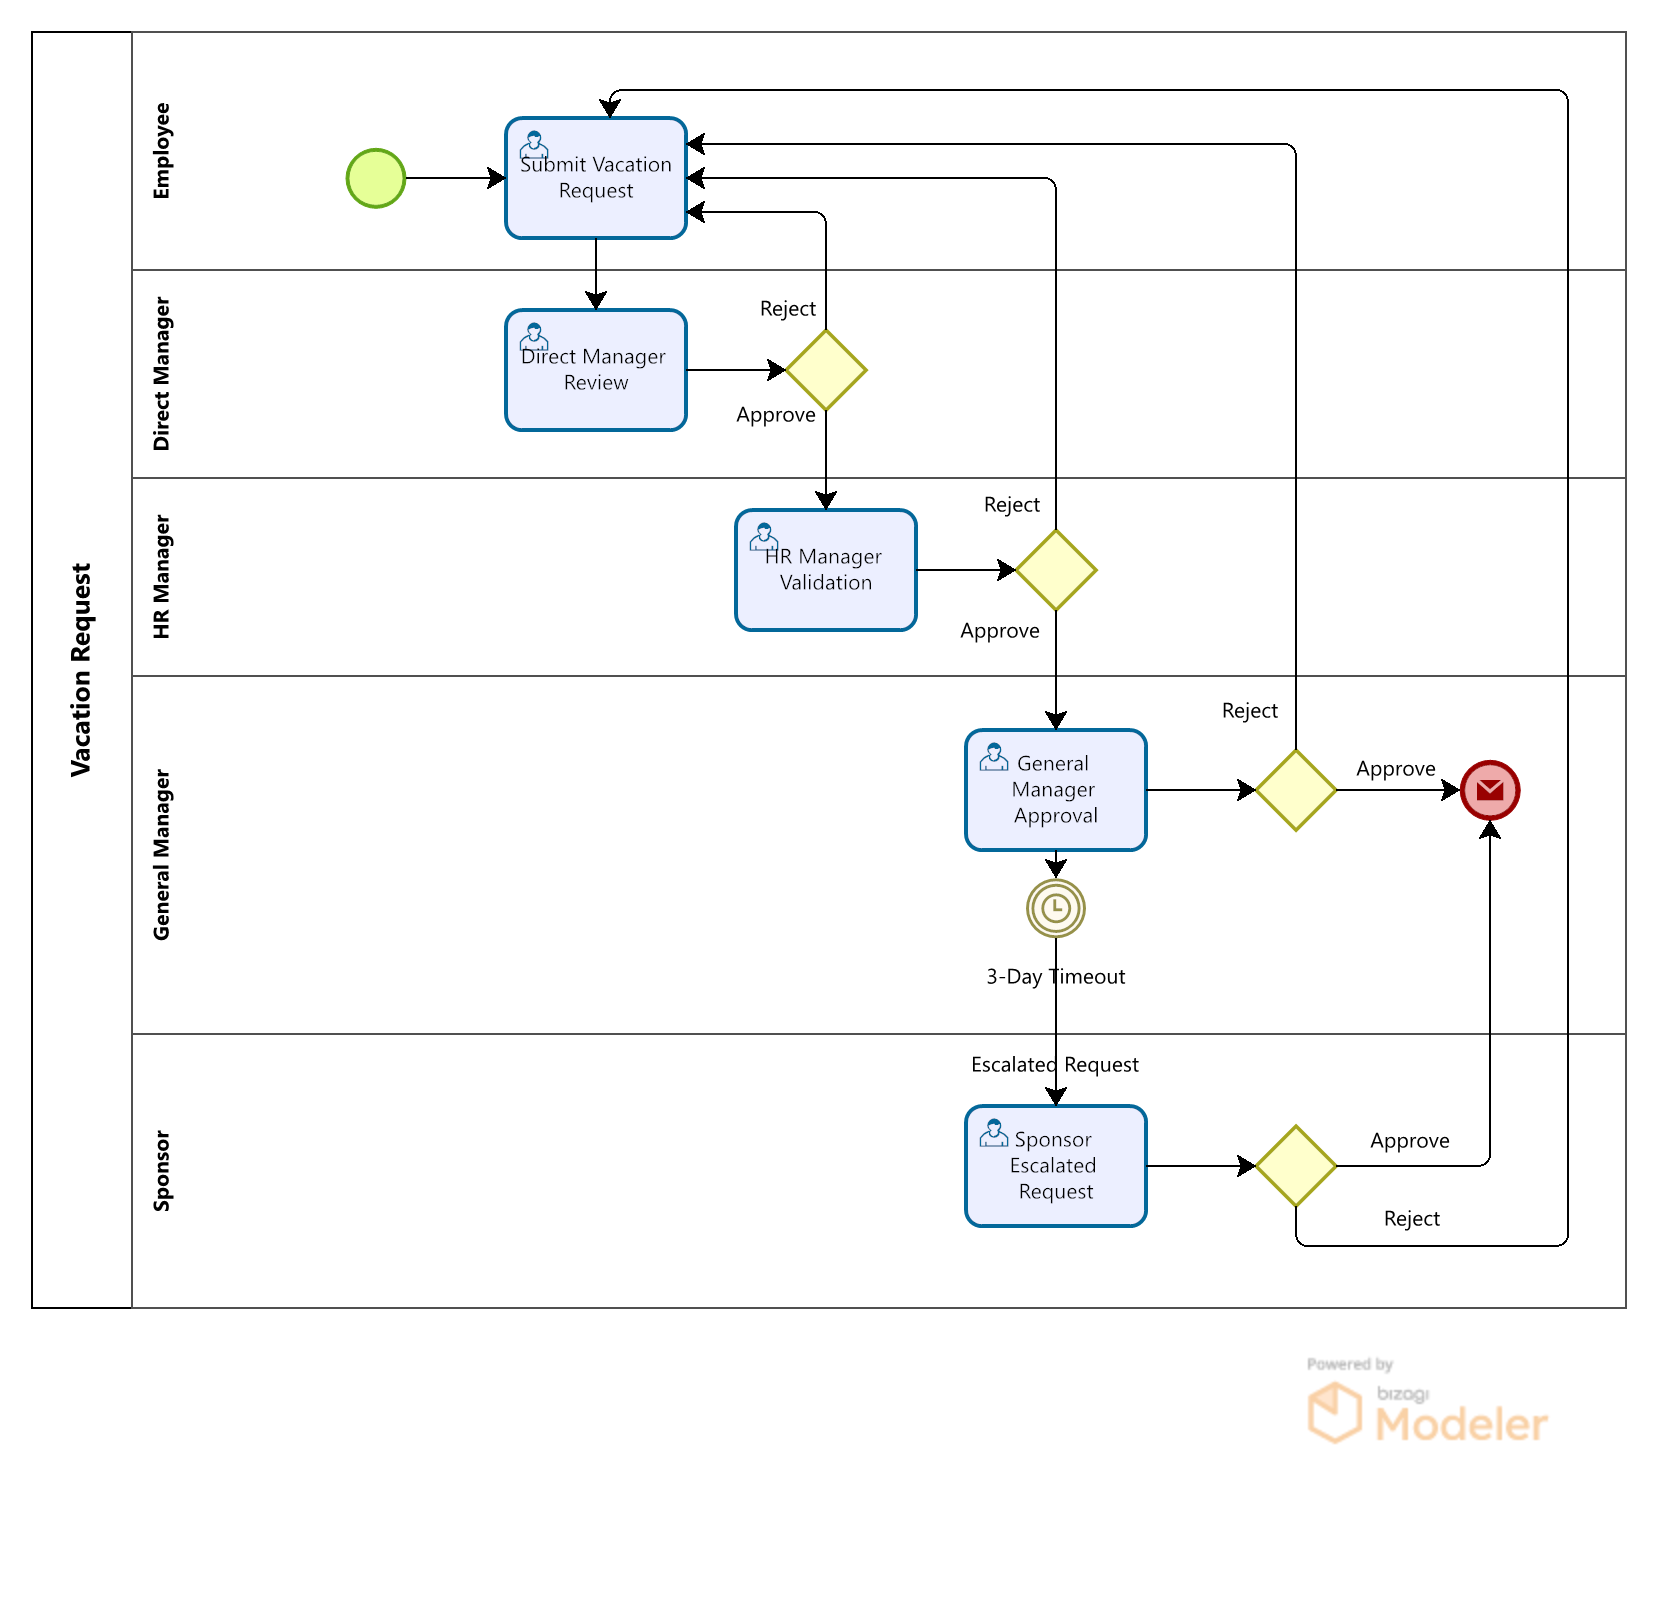
\includegraphics[width=0.9\textwidth]{Diagrams/Workflows/Vacation-Request-Escalation-to-Sponsor/Vacation-Request-Escalation-to-Sponsor.png}
\caption{Vacation Request Escalation to Sponsor Workflow - Automatic Escalation}
\label{fig:escalation-flow}
\end{figure}

\subsubsection{Resubmission After Rejection Flow}
Rejected requests can be resubmitted following this process:

\begin{figure}[H]
\centering
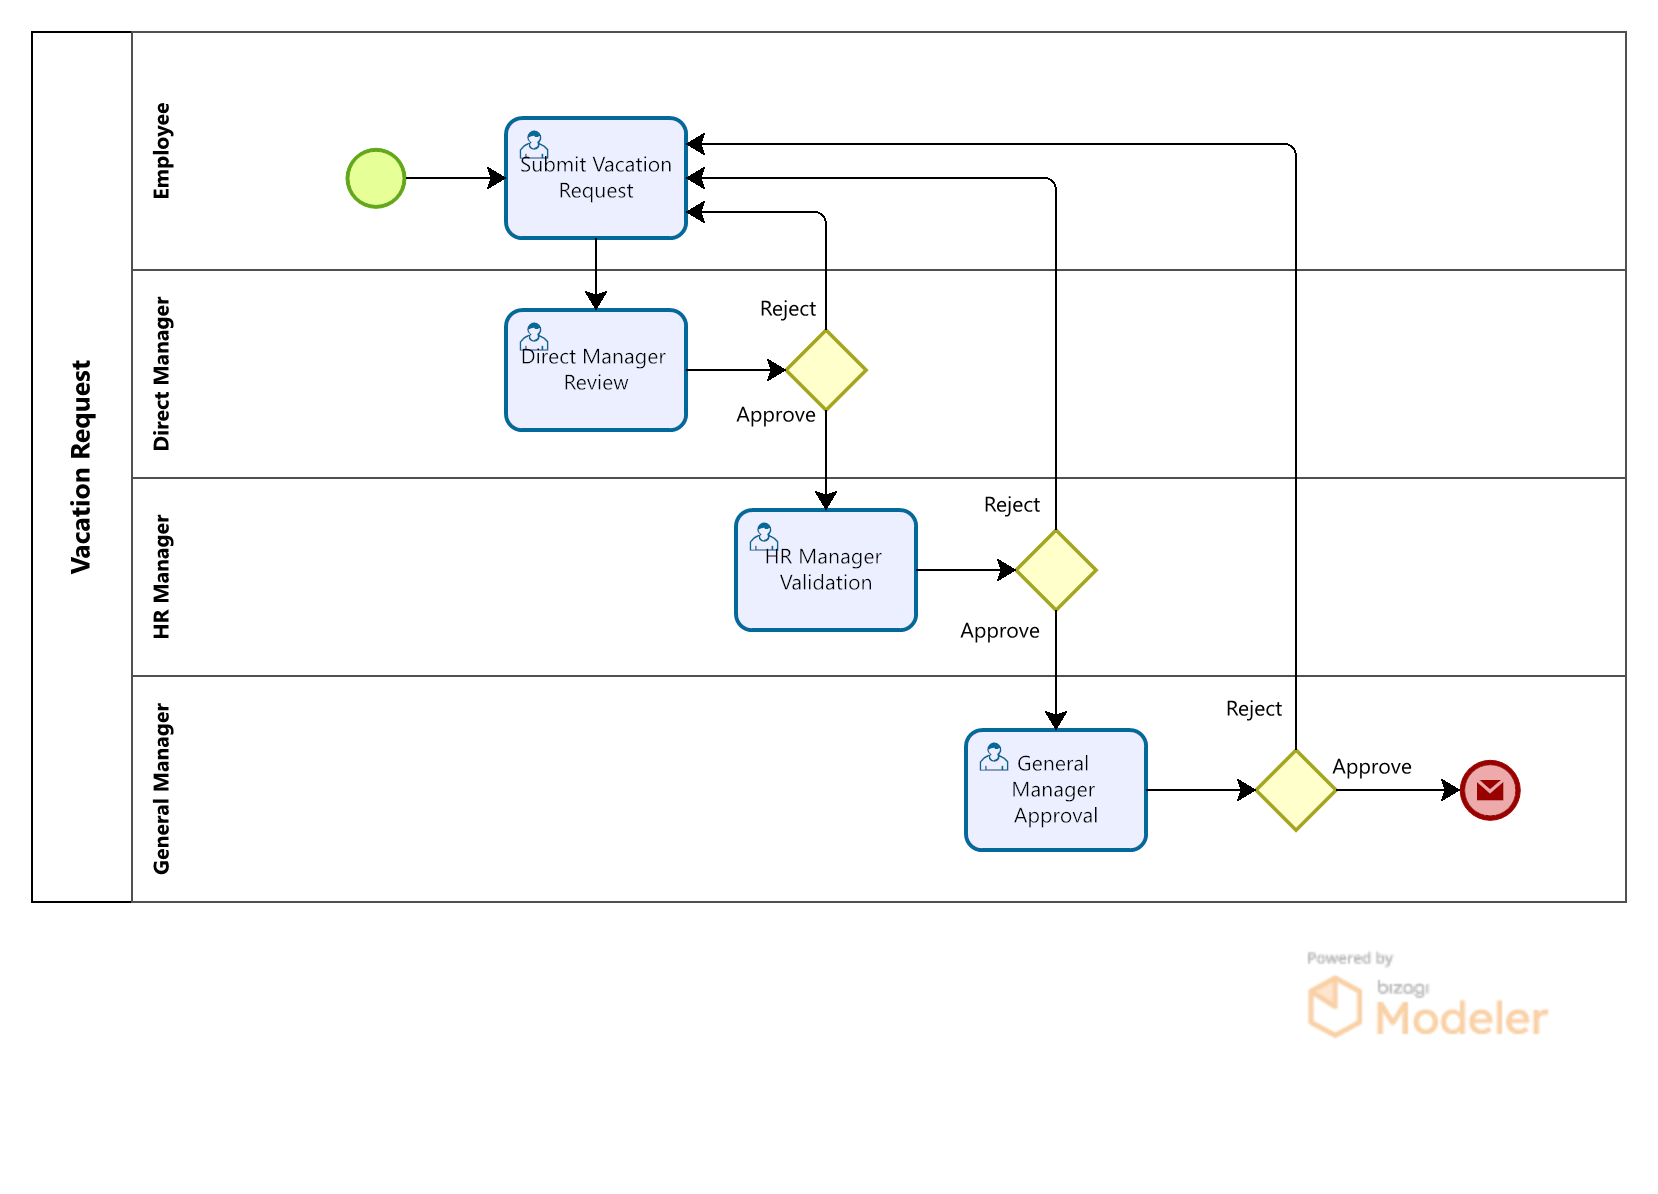
\includegraphics[width=0.9\textwidth]{Diagrams/Workflows/Vacation-Request-Resubmission-After-Rejection/Vacation-Request-Resubmission-After-Rejection.png}
\caption{Vacation Request Resubmission After Rejection Workflow}
\label{fig:resubmission-flow}
\end{figure}

\section{Business Rules and Logic}

This section consolidates all core business rules that govern the system's behavior. These rules are referenced by use cases and functional requirements throughout the document.

\subsection{Vacation Policy Rules}

\subsubsection{BR-001: Annual Entitlement}
\textbf{Rule}: Standard annual vacation entitlement is 21 days per year.
\textbf{Applicable Use Cases}: UC-1, UC-12
\textbf{Implementation}: System automatically allocates 21 days at the start of each calendar year.

\subsubsection{BR-002: Extended Entitlement}
\textbf{Rule}: Employees with 10+ years of service OR age >= 50 receive 30 days annual entitlement.
\textbf{Applicable Use Cases}: UC-1, UC-12
\textbf{Implementation}: System evaluates hire date and birth date from Employee Master Data to determine eligibility.

\subsubsection{BR-003: Leave Types}
\textbf{Rule}: System supports only Annual and Sick leave types.
\textbf{Applicable Use Cases}: UC-1, UC-4, UC-5
\textbf{Implementation}: Vacation Types Master Data defines these two types exclusively.

\subsubsection{BR-004: Unused Days Policy}
\textbf{Rule}: Unused vacation days are forfeited annually with no carryover or compensation.
\textbf{Applicable Use Cases}: UC-12
\textbf{Implementation}: System resets balance to annual entitlement at year-end without preserving unused days.

\subsubsection{BR-005: Trainee Restrictions}
\textbf{Rule}: Trainees cannot submit vacation requests.
\textbf{Applicable Use Cases}: UC-1
\textbf{Implementation}: System checks employee status from Employee Master Data and blocks request submission for trainees.

\subsection{Approval Workflow Rules}

\subsubsection{BR-006: Approval Hierarchy}
\textbf{Rule}: Vacation requests follow the sequence: Employee → Direct Manager → HR → General Manager.
\textbf{Applicable Use Cases}: UC-1, UC-4, UC-6
\textbf{Implementation}: System routes requests through predefined approval levels with role-based access control.

\subsubsection{BR-007: Escalation Policy}
\textbf{Rule}: Requests automatically escalate to the next level after 2 days of inaction.
\textbf{Applicable Use Cases}: UC-4, UC-6
\textbf{Implementation}: System timer tracks approval delays and automatically forwards requests.

\subsubsection{BR-008: Balance Update Timing}
\textbf{Rule}: Employee vacation balance updates only after General Manager approval.
\textbf{Applicable Use Cases}: UC-4, UC-12
\textbf{Implementation}: System triggers balance recalculation upon GM approval, not at earlier stages.

\subsubsection{BR-009: Rejection Documentation}
\textbf{Rule}: All rejections must include a mandatory reason.
\textbf{Applicable Use Cases}: UC-4, UC-5
\textbf{Implementation}: System validates that reason field is populated before allowing rejection submission.

\subsubsection{BR-010: No Modification Policy}
\textbf{Rule}: Submitted vacation requests cannot be modified.
\textbf{Applicable Use Cases}: UC-1
\textbf{Implementation}: System locks all request fields after submission, allowing only cancellation.

\subsection{Validation Rules}

\subsubsection{BR-011: Date Validation}
\textbf{Rule}: Start date must be in the future, and end date must be after start date.
\textbf{Applicable Use Cases}: UC-1
\textbf{Implementation}: System validates date inputs in real-time and prevents submission of invalid dates.

\subsubsection{BR-012: Overlap Prevention}
\textbf{Rule}: No overlapping vacation requests are allowed for the same employee.
\textbf{Applicable Use Cases}: UC-1
\textbf{Implementation}: System checks existing requests against proposed dates and blocks submission if conflicts exist.

\subsubsection{BR-013: Balance Validation}
\textbf{Rule}: Requested vacation days must not exceed available leave balance.
\textbf{Applicable Use Cases}: UC-1
\textbf{Implementation}: System calculates available balance (Total - Taken - Pending) and validates against request.

\subsubsection{BR-014: Attachment Requirements}
\textbf{Rule}: Medical certificates are mandatory for sick leave requests.
\textbf{Applicable Use Cases}: UC-1, UC-4
\textbf{Implementation}: System requires file upload for sick leave type and validates attachment presence.

\subsubsection{BR-015: Cancellation Eligibility}
\textbf{Rule}: Only requests in Pending or Approved status can be cancelled.
\textbf{Applicable Use Cases}: UC-2, UC-3, UC-5
\textbf{Implementation}: System checks request status and enables/disables cancellation functionality accordingly.

\subsubsection{BR-016: Cancellation Timing}
\textbf{Rule}: Cancellation must occur before vacation start date.
\textbf{Applicable Use Cases}: UC-2, UC-5
\textbf{Implementation}: System compares current date with vacation start date and blocks late cancellations.

\subsection{System Behavior Rules}

\subsubsection{BR-017: Notification Delivery}
\textbf{Rule}: System must notify all stakeholders of status changes within 5 minutes.
\textbf{Applicable Use Cases}: UC-1, UC-2, UC-4, UC-5, UC-11
\textbf{Implementation}: Real-time notification system triggers alerts upon workflow state changes.

\subsubsection{BR-018: Data Integrity}
\textbf{Rule}: All vacation transactions must maintain complete audit trail.
\textbf{Applicable Use Cases}: All UC
\textbf{Implementation}: System logs all actions with timestamp, user ID, and action details.

\subsubsection{BR-019: Policy Configuration}
\textbf{Rule}: Vacation policies must be configurable through administrative interface.
\textbf{Applicable Use Cases}: UC-12
\textbf{Implementation}: System provides configuration screens for entitlement days, eligibility criteria, and escalation timeframes.

\section{User Requirements / Use Cases}

This section provides high-level descriptions of the system's use cases. For detailed specifications, including triggers, basic/alternate flows, business validation rules, non-functional constraints, and exceptions, please refer to the All-UseCases.json document.

\subsection{Use Case Summary}
The system implements 12 core use cases that cover all aspects of vacation management:

\begin{table}[H]
\centering
\begin{tabular}{|p{1cm}|p{4cm}|p{3cm}|p{3cm}|}
\hline
\textbf{ID} & \textbf{Use Case Name} & \textbf{Primary Actor} & \textbf{Business Rules} \\
\hline
UC-1 & Employee Submits Vacation Request & Employee & BR-001, BR-002, BR-003, BR-011, BR-012, BR-013, BR-014 \\
\hline
UC-2 & Employee Submits Vacation Cancellation Request & Employee & BR-015, BR-016 \\
\hline
UC-3 & My Vacation Requests & Employee & BR-015, BR-016 \\
\hline
UC-4 & Review Vacation Request (Approval/Rejection) & Manager/HR/GM & BR-006, BR-007, BR-008, BR-009, BR-014 \\
\hline
UC-5 & Review Vacation Cancellation Request & Manager/HR & BR-015, BR-016, BR-009 \\
\hline
UC-6 & Pending Vacation Requests & Manager/HR & BR-006, BR-007 \\
\hline
UC-7 & Vacation Inquiry (Search Parameters) & HR/Managers/Employees & BR-018 \\
\hline
UC-8 & Vacation Inquiry (Search Results) & HR/Managers/Employees & BR-018 \\
\hline
UC-9 & Print Single Vacation Transaction Report (PDF) & HR/Managers/Employees & BR-018 \\
\hline
UC-10 & Print Comparative Annual Report (PDF) & HR/Managers/GM & BR-018 \\
\hline
UC-11 & Notifications Center & All Users & BR-017 \\
\hline
UC-12 & Automated Update of Employee Annual Vacation Balance & System & BR-001, BR-002, BR-008, BR-019 \\
\hline
\end{tabular}
\caption{Use Case Summary with Business Rule References}
\end{table}

\subsection{Use Case Details}
The following use cases are implemented in the system:

\subsubsection{UC-1: Employee Submits Vacation Request}
\begin{figure}[H]
\centering
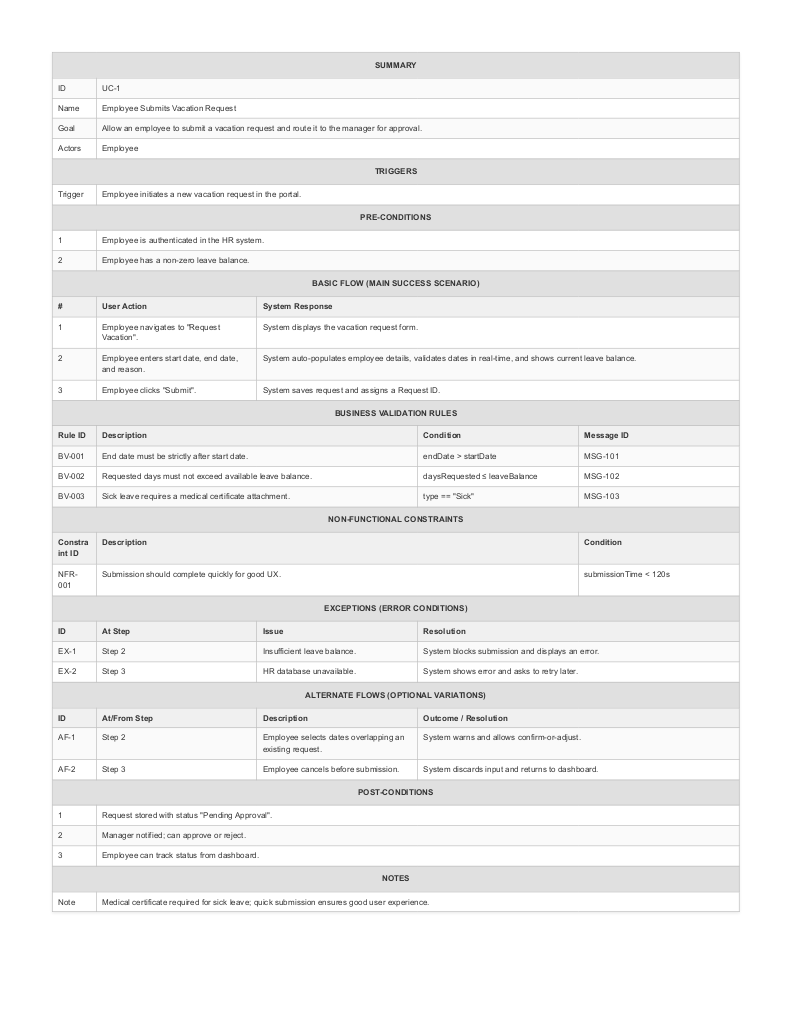
\includegraphics[width=0.9\textwidth]{Use-Cases/UC-1-Employee-Vacation-Request/UC-1-Employee-Vacation-Request-1.png}
\caption{UC-1: Employee Vacation Request Use Case}
\label{fig:uc1}
\end{figure}

\subsubsection{UC-2: Employee Submits Vacation Cancellation Request}
\begin{figure}[H]
\centering
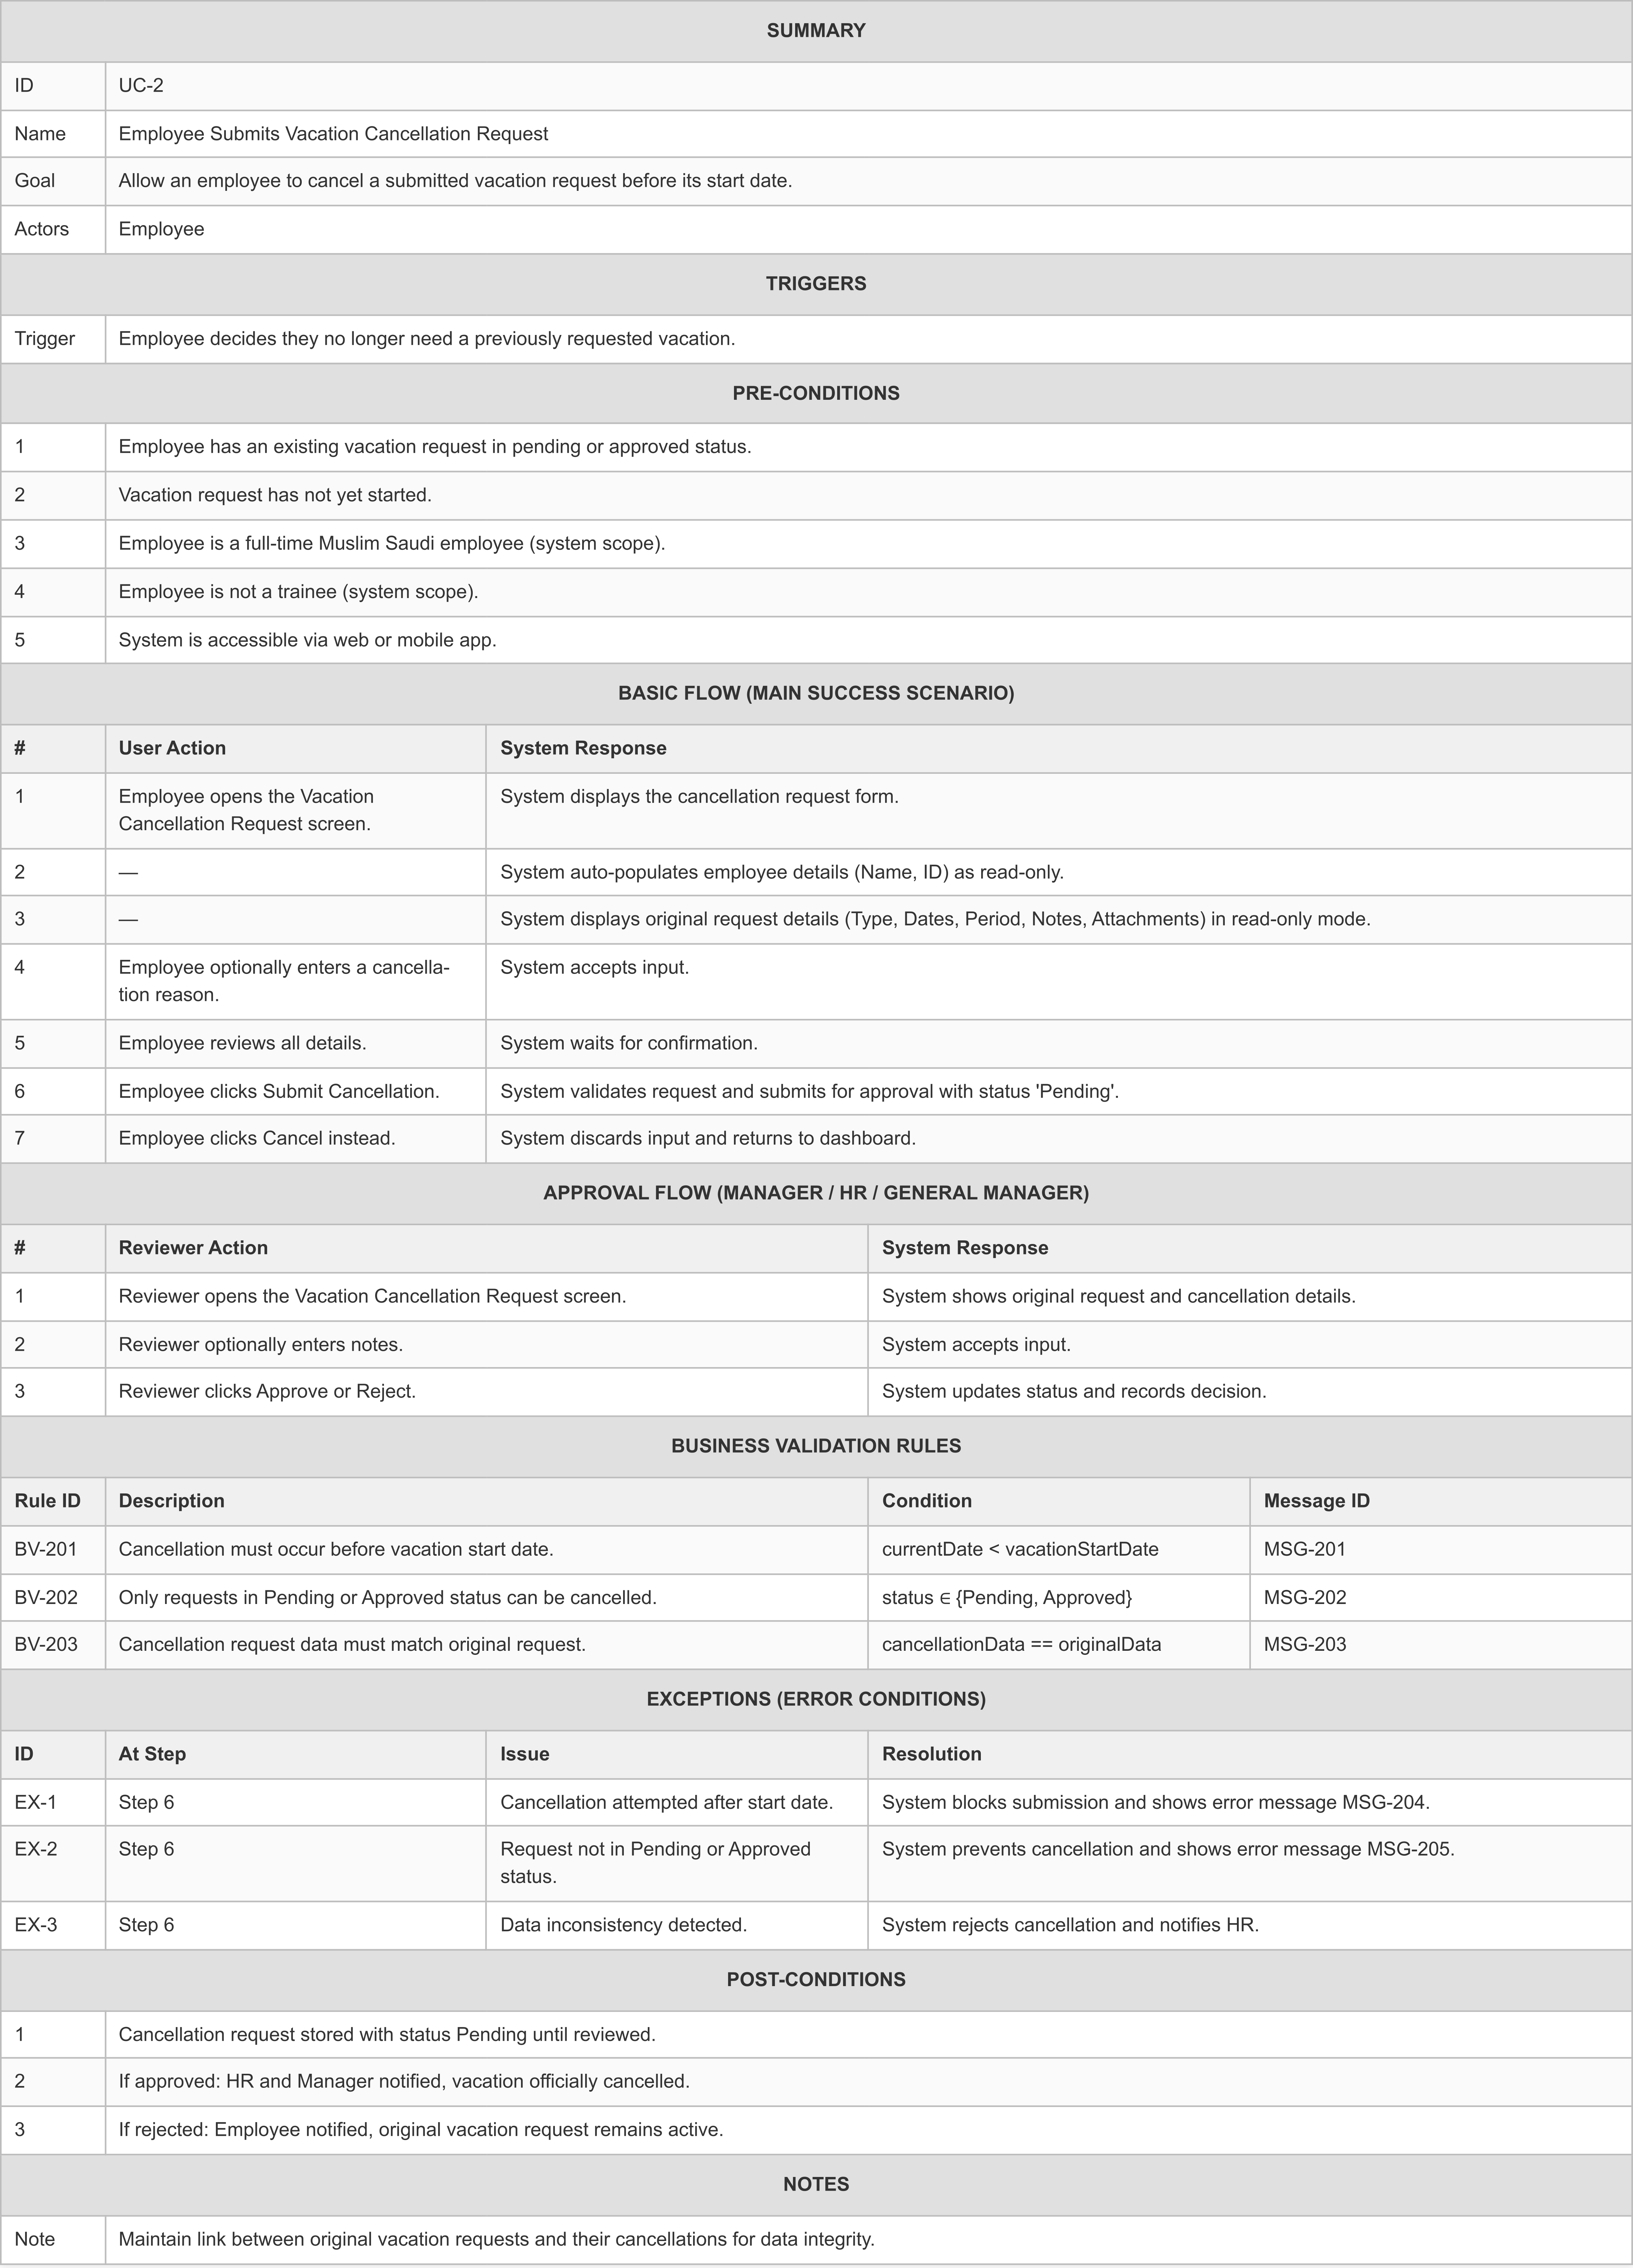
\includegraphics[width=0.9\textwidth]{Use-Cases/UC-2-Employee-Vacation-Cancellation-Request/UC-2-Employee-Vacation-Cancellation-Request-1.png}
\caption{UC-2: Employee Vacation Cancellation Request Use Case}
\label{fig:uc2}
\end{figure}

\subsubsection{UC-3: My Vacation Requests}
\begin{figure}[H]
\centering
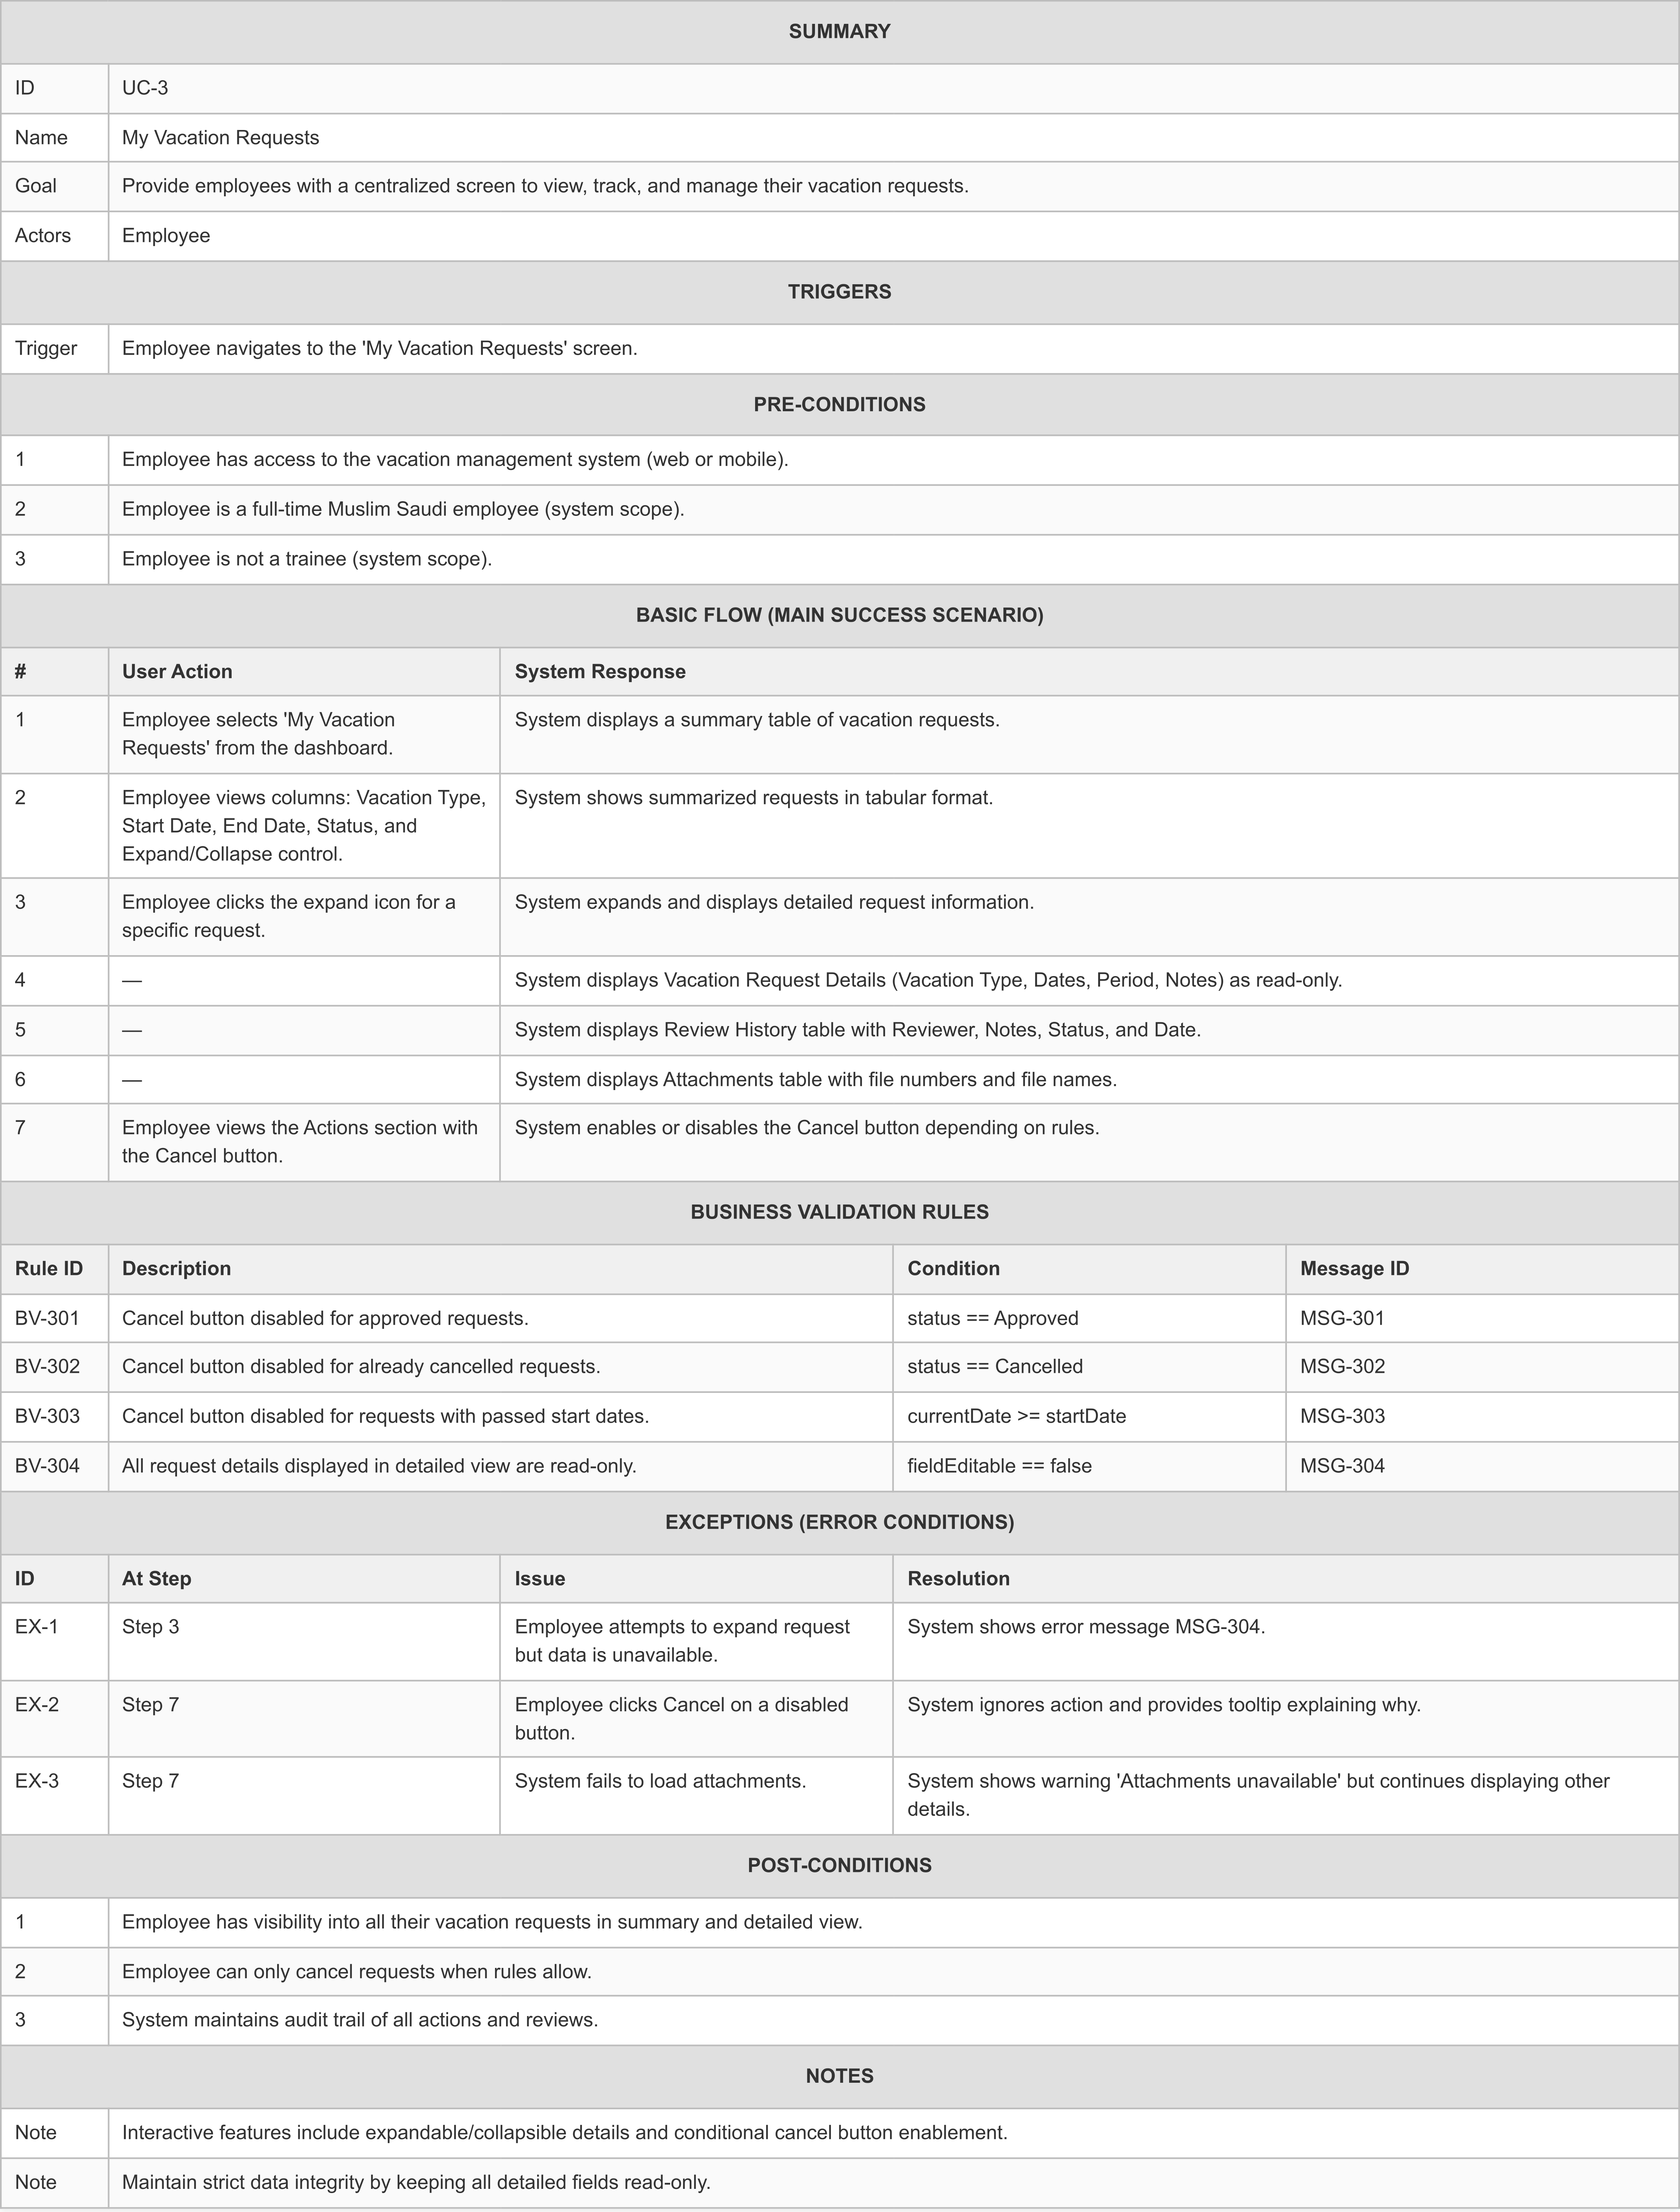
\includegraphics[width=0.9\textwidth]{Use-Cases/UC-3-My-Vacation-Requests/UC-3-My-Vacation-Requests-1.png}
\caption{UC-3: My Vacation Requests Use Case}
\label{fig:uc3}
\end{figure}

\subsubsection{UC-4: Review Vacation Request (Approval/Rejection)}
\begin{figure}[H]
\centering
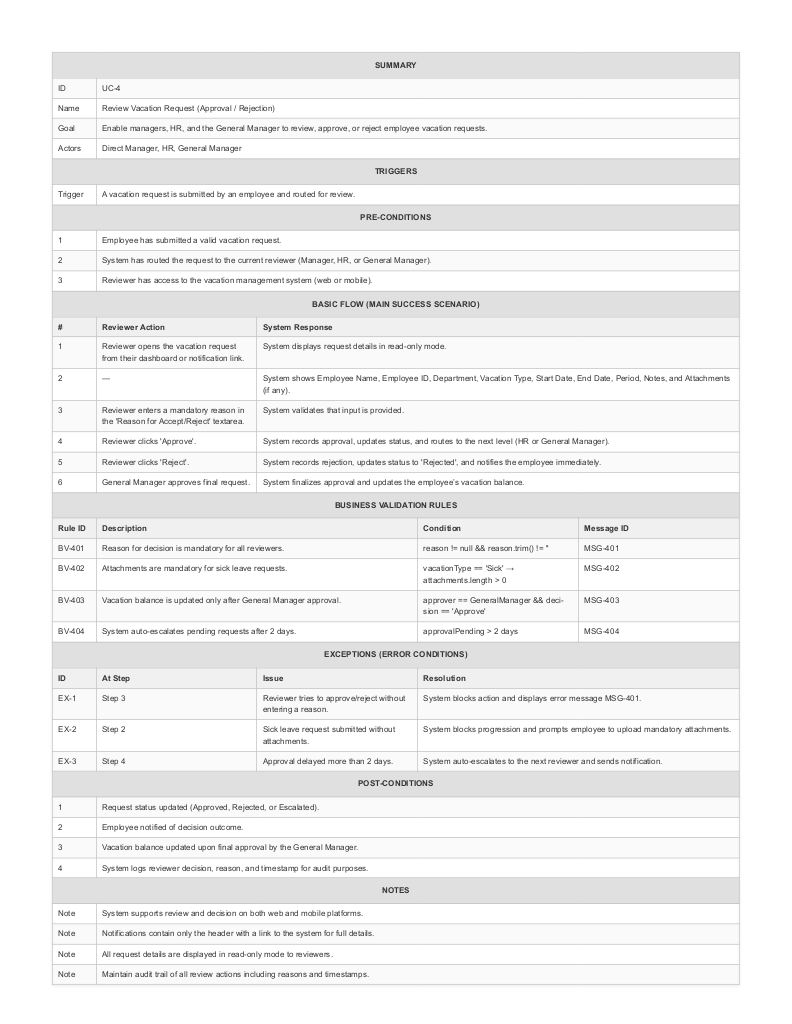
\includegraphics[width=0.9\textwidth]{Use-Cases/UC-4-Review-Vacation-Request/UC-4-Review-Vacation-Request-1.png}
\caption{UC-4: Review Vacation Request Use Case}
\label{fig:uc4}
\end{figure}

\subsubsection{UC-5: Review Vacation Cancellation Request}
\begin{figure}[H]
\centering
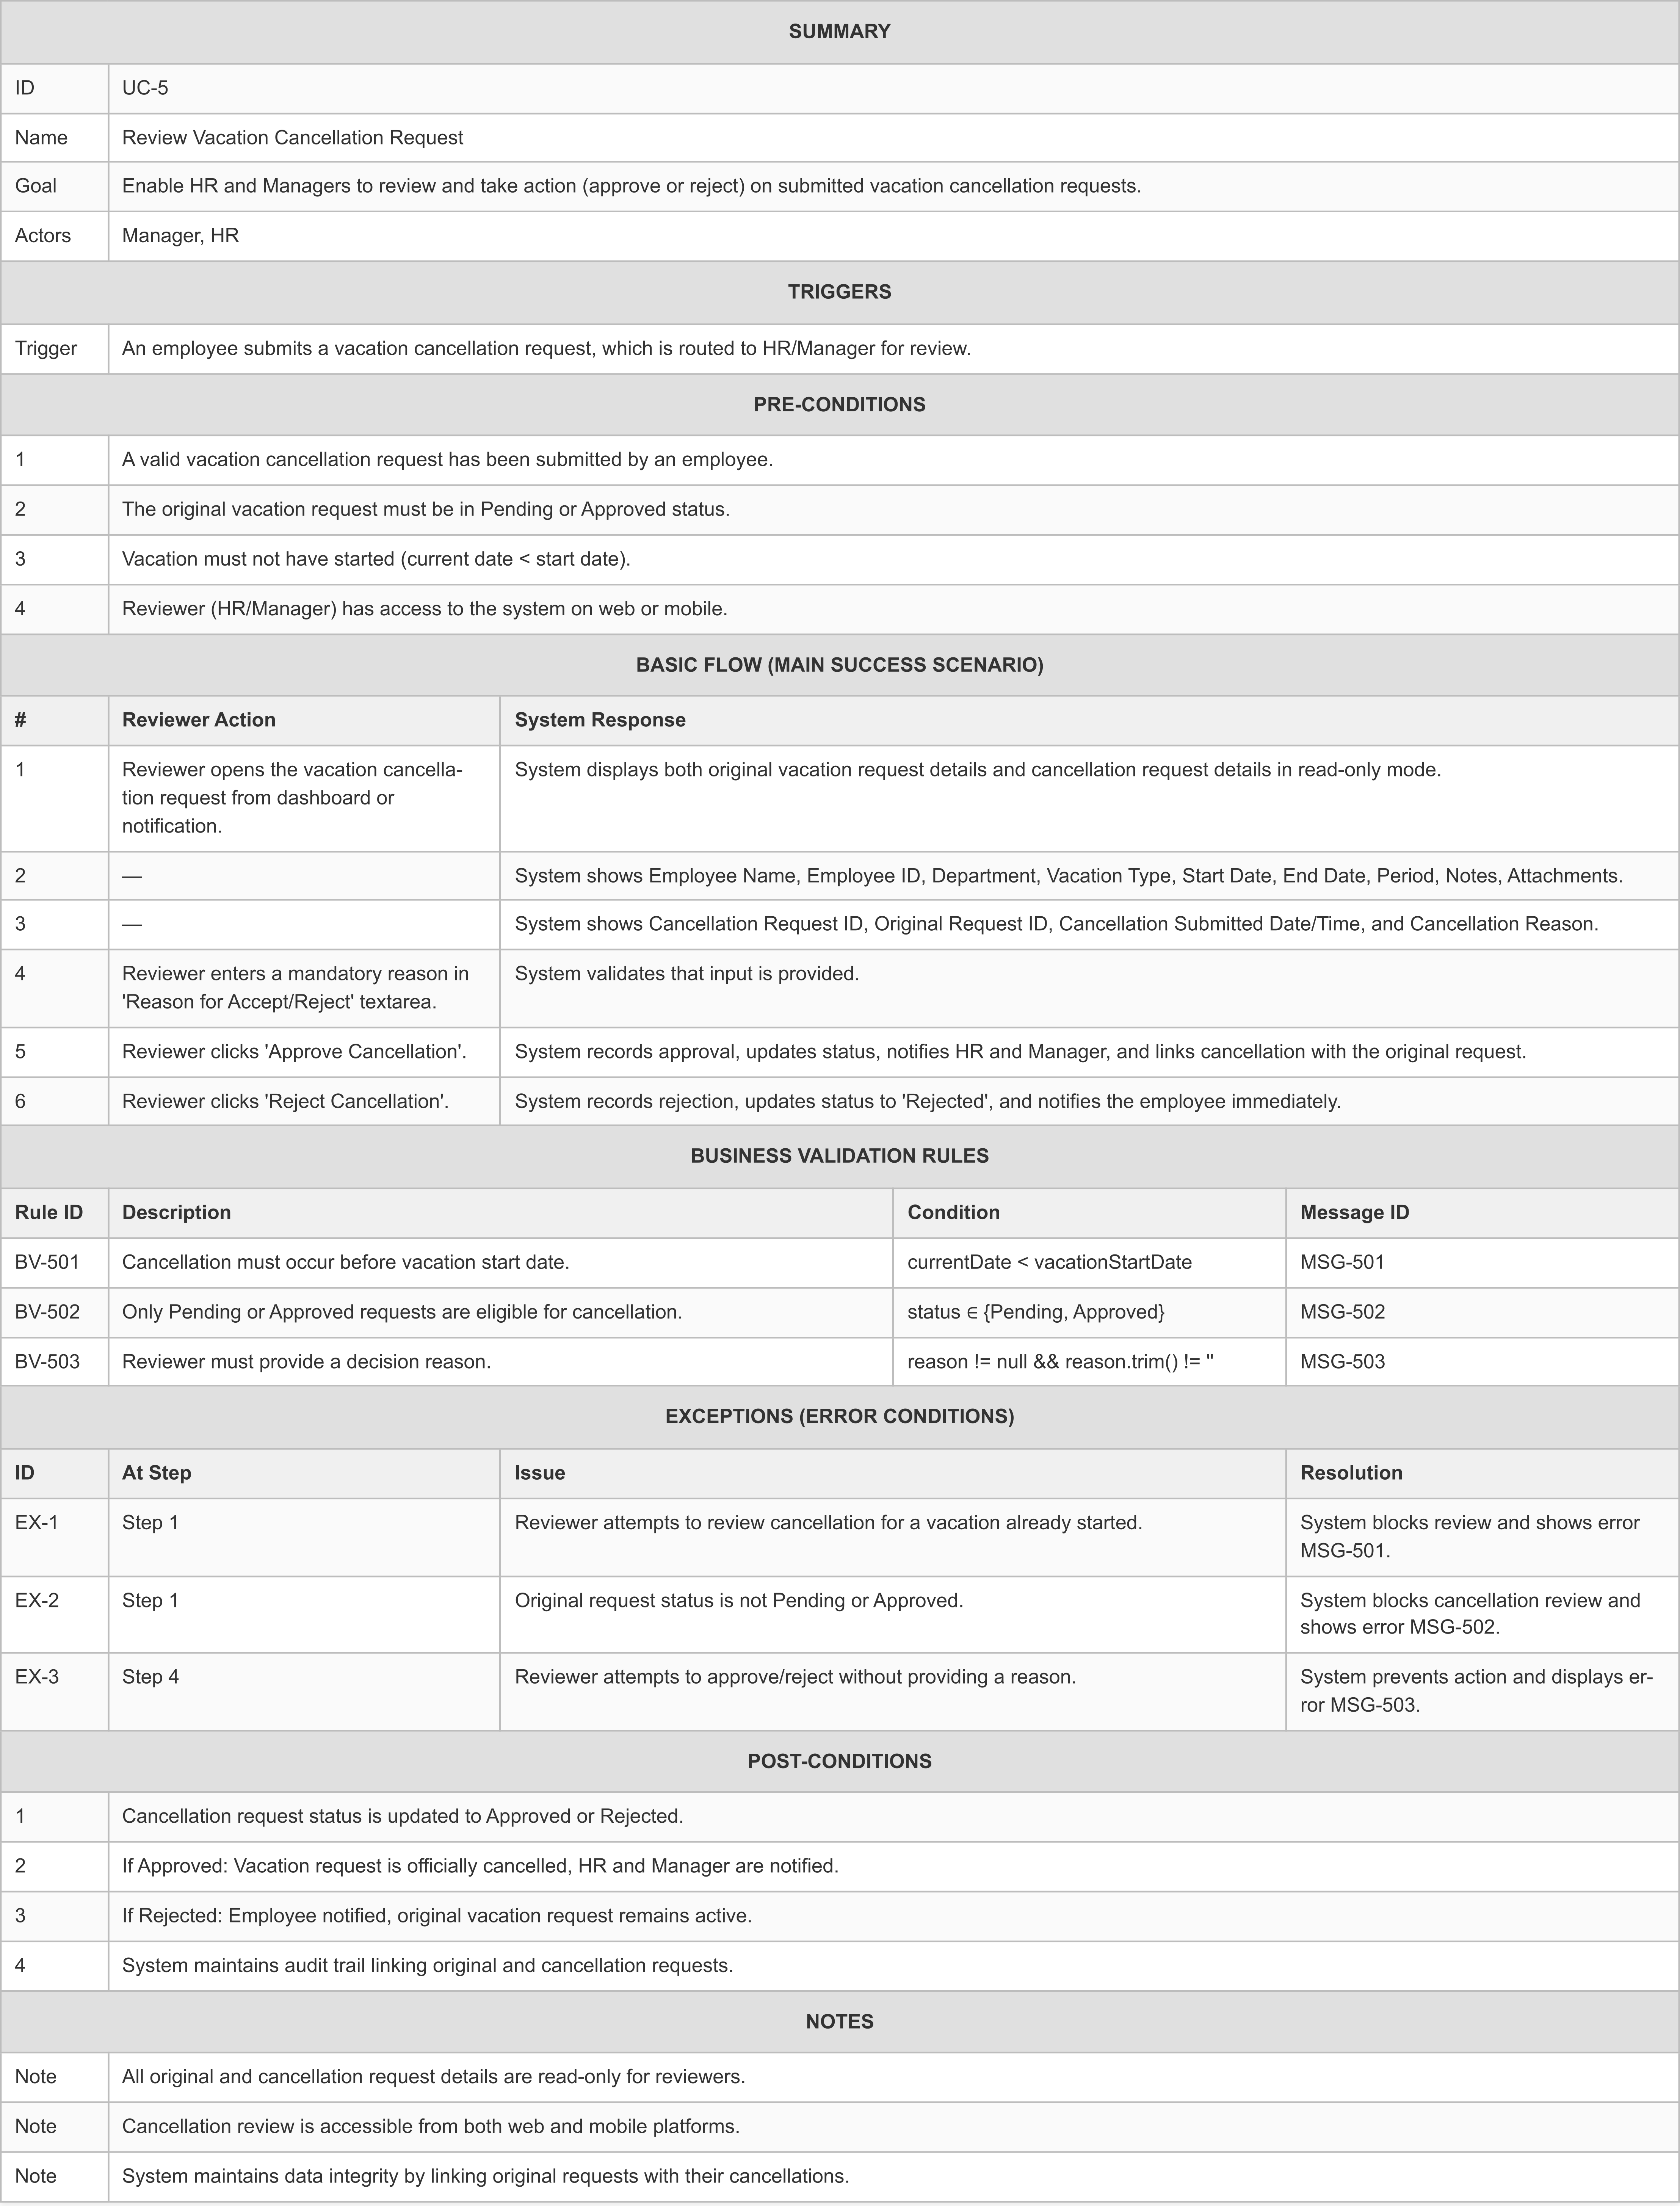
\includegraphics[width=0.9\textwidth]{Use-Cases/UC-5-Review-Vacation-Cancellation-Request/UC-5-Review-Vacation-Cancellation-Request-1.png}
\caption{UC-5: Review Vacation Cancellation Request Use Case}
\label{fig:uc5}
\end{figure}

\subsubsection{UC-6: Pending Vacation Requests}
\begin{figure}[H]
\centering
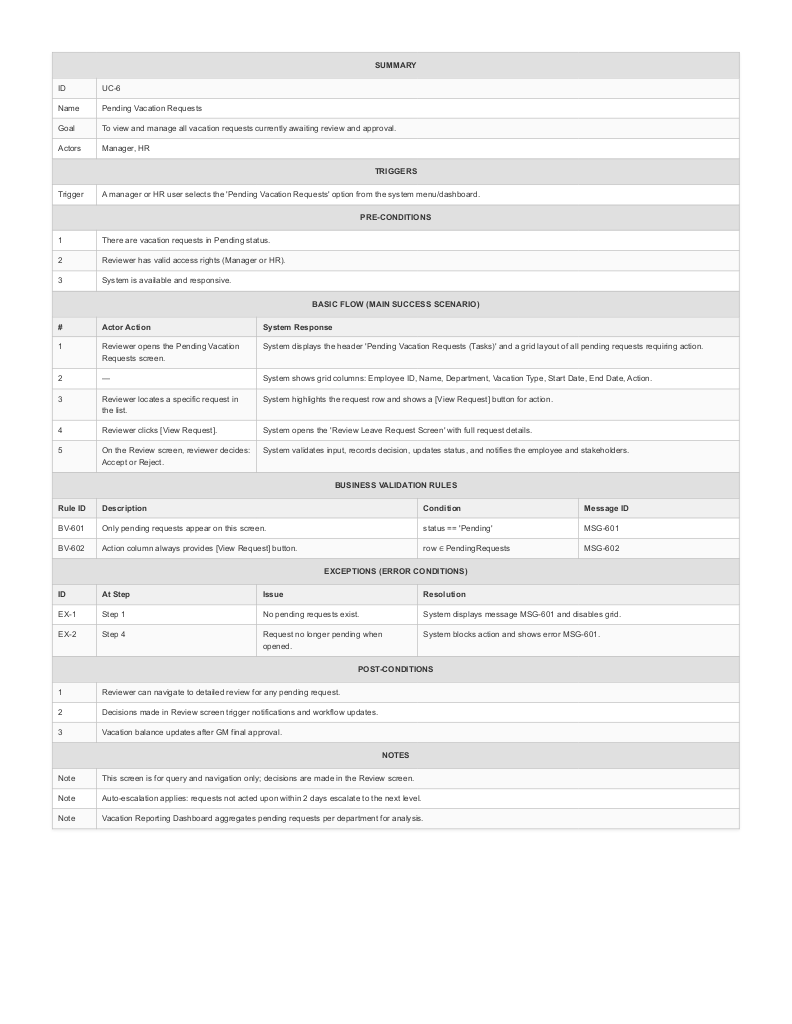
\includegraphics[width=0.9\textwidth]{Use-Cases/UC-6-Pending-Vacation-Requests/UC-6-Pending-Vacation-Requests-1.png}
\caption{UC-6: Pending Vacation Requests Use Case}
\label{fig:uc6}
\end{figure}

\subsubsection{UC-7: Vacation Inquiry (Search Parameters)}
\begin{figure}[H]
\centering
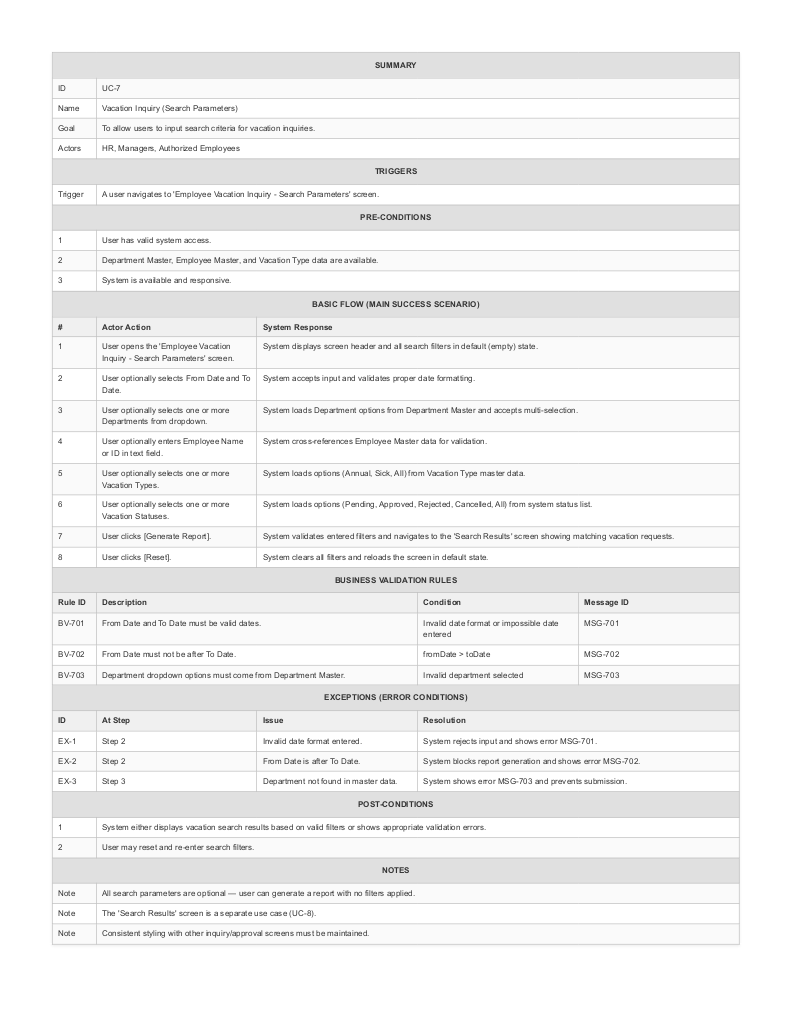
\includegraphics[width=0.9\textwidth]{Use-Cases/UC-7-Vacation-Inquiry-Search-Parameters/UC-7-Vacation-Inquiry-Search-Parameters-1.png}
\caption{UC-7: Vacation Inquiry Search Parameters Use Case}
\label{fig:uc7}
\end{figure}

\subsubsection{UC-8: Vacation Inquiry (Search Results)}
\begin{figure}[H]
\centering
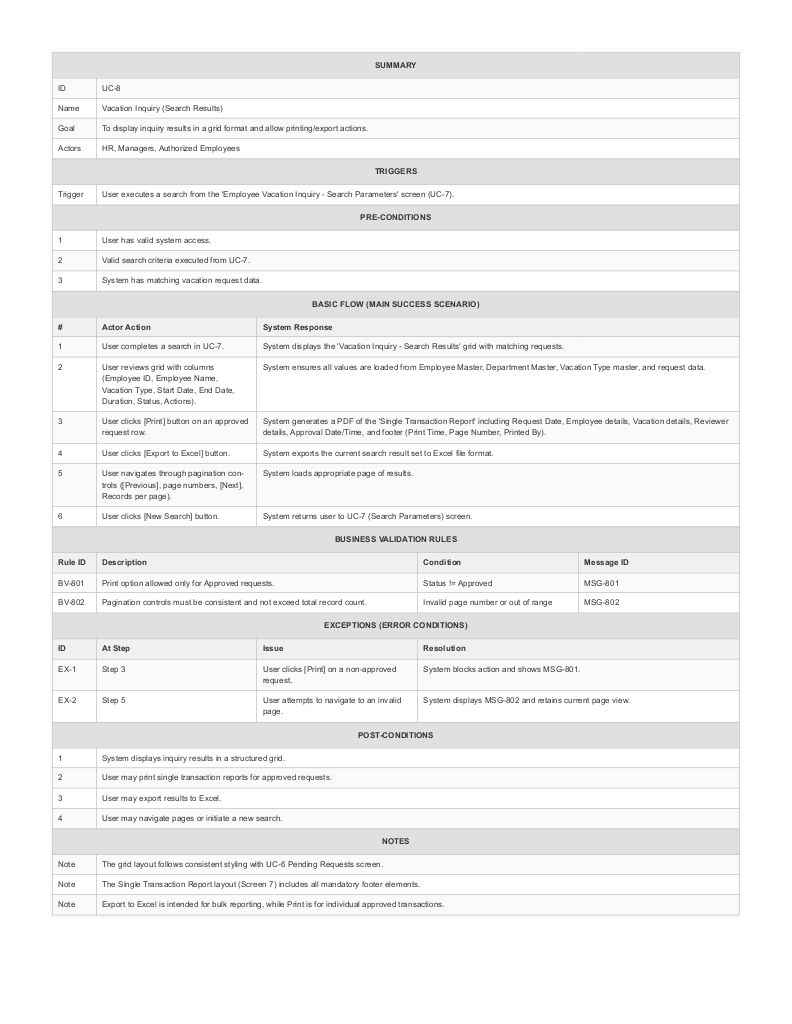
\includegraphics[width=0.9\textwidth]{Use-Cases/UC-8-Vacation-Inquiry-Search-Results/UC-8-Vacation-Inquiry-Search-Results-1.png}
\caption{UC-8: Vacation Inquiry Search Results Use Case}
\label{fig:uc8}
\end{figure}

\subsubsection{UC-9: Print Single Vacation Transaction Report (PDF)}
\begin{figure}[H]
\centering
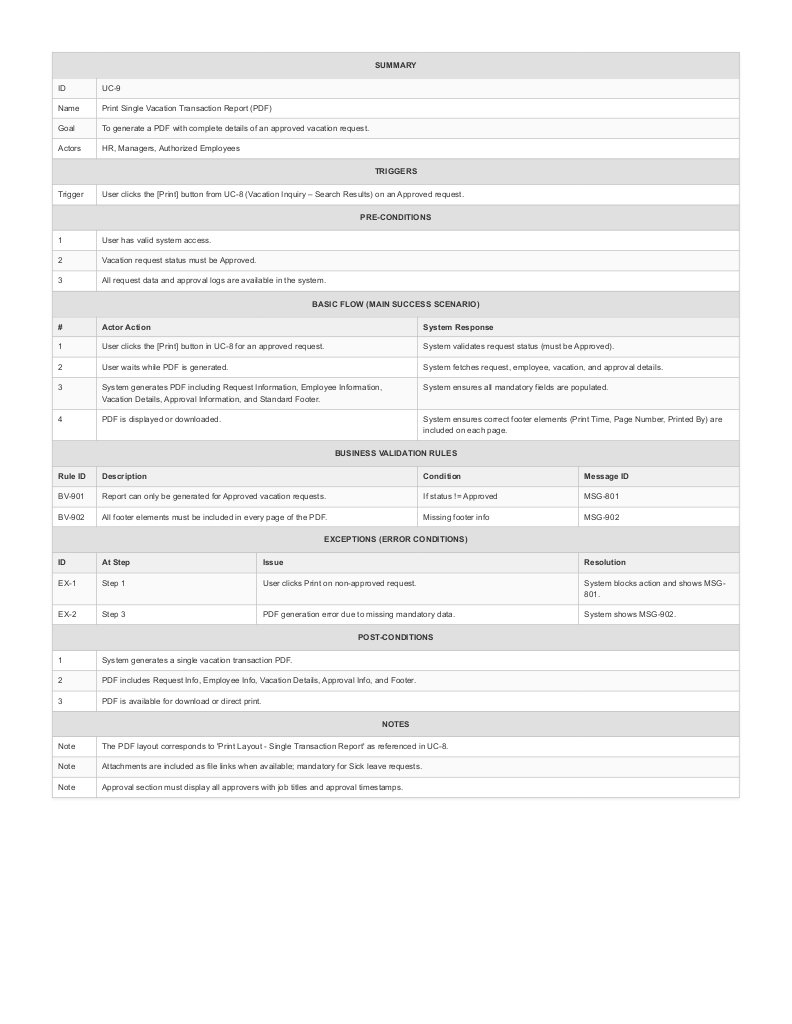
\includegraphics[width=0.9\textwidth]{Use-Cases/UC-9-Print-Single-Vacation-Transaction-Report/UC-9-Print-Single-Vacation-Transaction-Report-1.png}
\caption{UC-9: Print Single Vacation Transaction Report Use Case}
\label{fig:uc9}
\end{figure}

\subsubsection{UC-10: Print Comparative Annual Report (PDF)}
\begin{figure}[H]
\centering
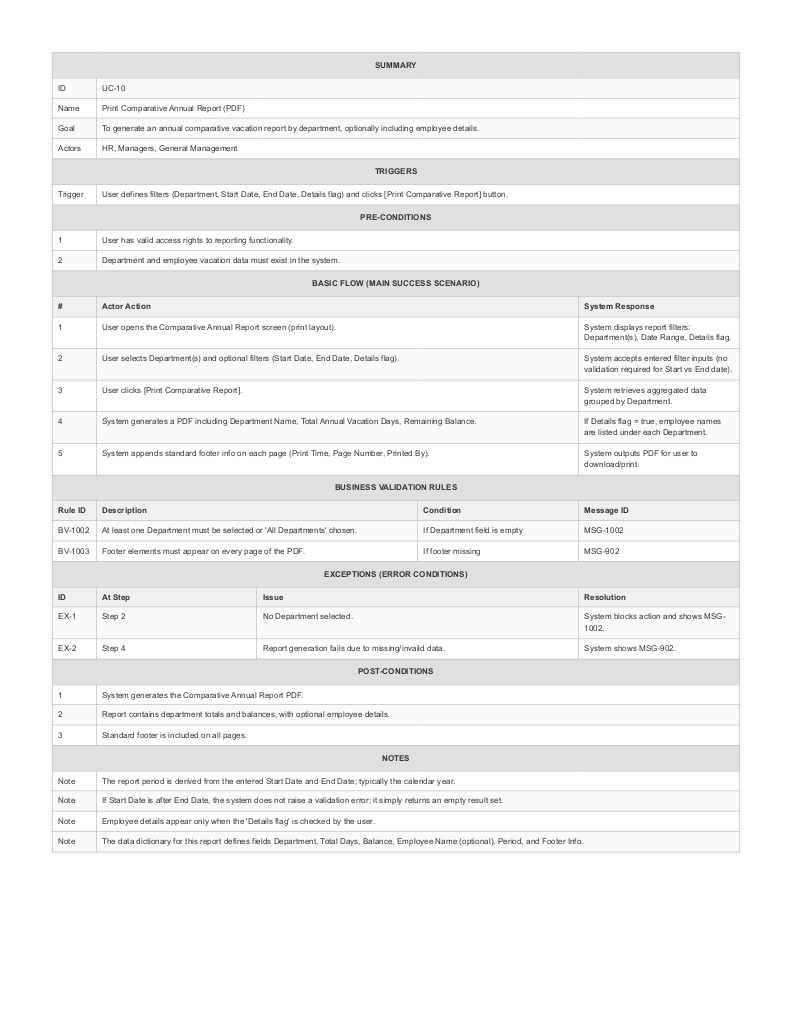
\includegraphics[width=0.9\textwidth]{Use-Cases/UC-10-Print-Comparative-Annual-Report/UC-10-Print-Comparative-Annual-Report-1.png}
\caption{UC-10: Print Comparative Annual Report Use Case}
\label{fig:uc10}
\end{figure}

\subsubsection{UC-11: Notifications Center}
\begin{figure}[H]
\centering
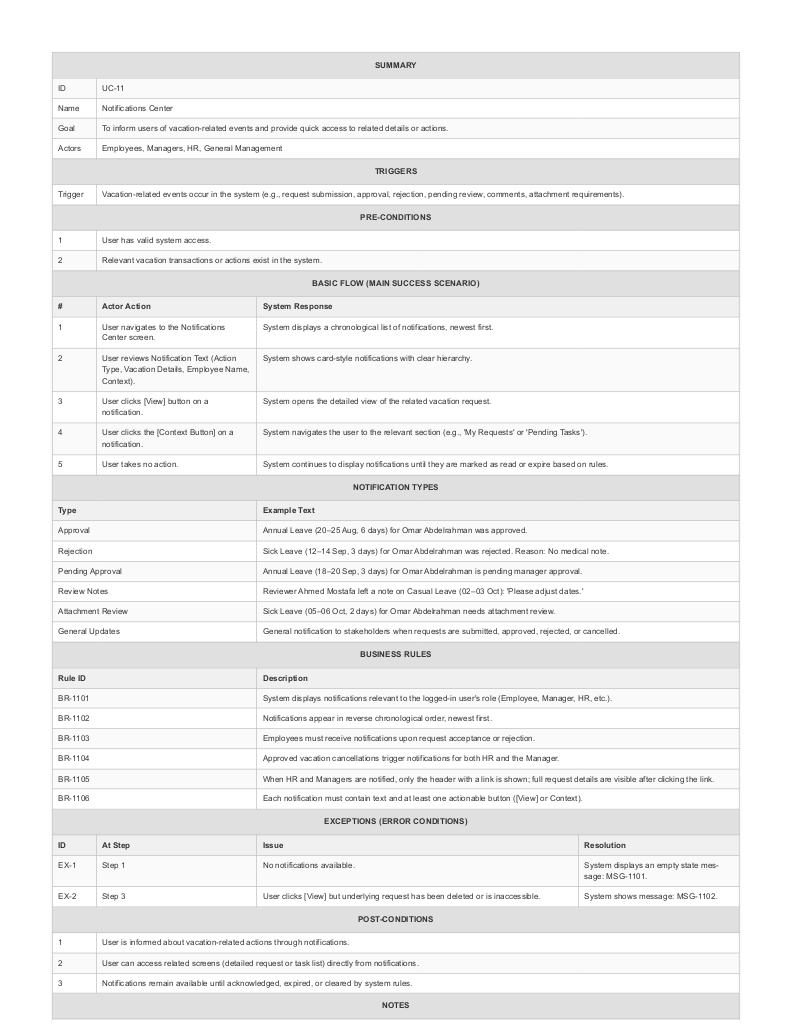
\includegraphics[width=0.9\textwidth]{Use-Cases/UC-11-Notifications-Center/UC-11-Notifications-Center-1.png}
\caption{UC-11: Notifications Center Use Case}
\label{fig:uc11}
\end{figure}

\subsubsection{UC-12: Automated Update of Employee Annual Vacation Balance}
\begin{figure}[H]
\centering
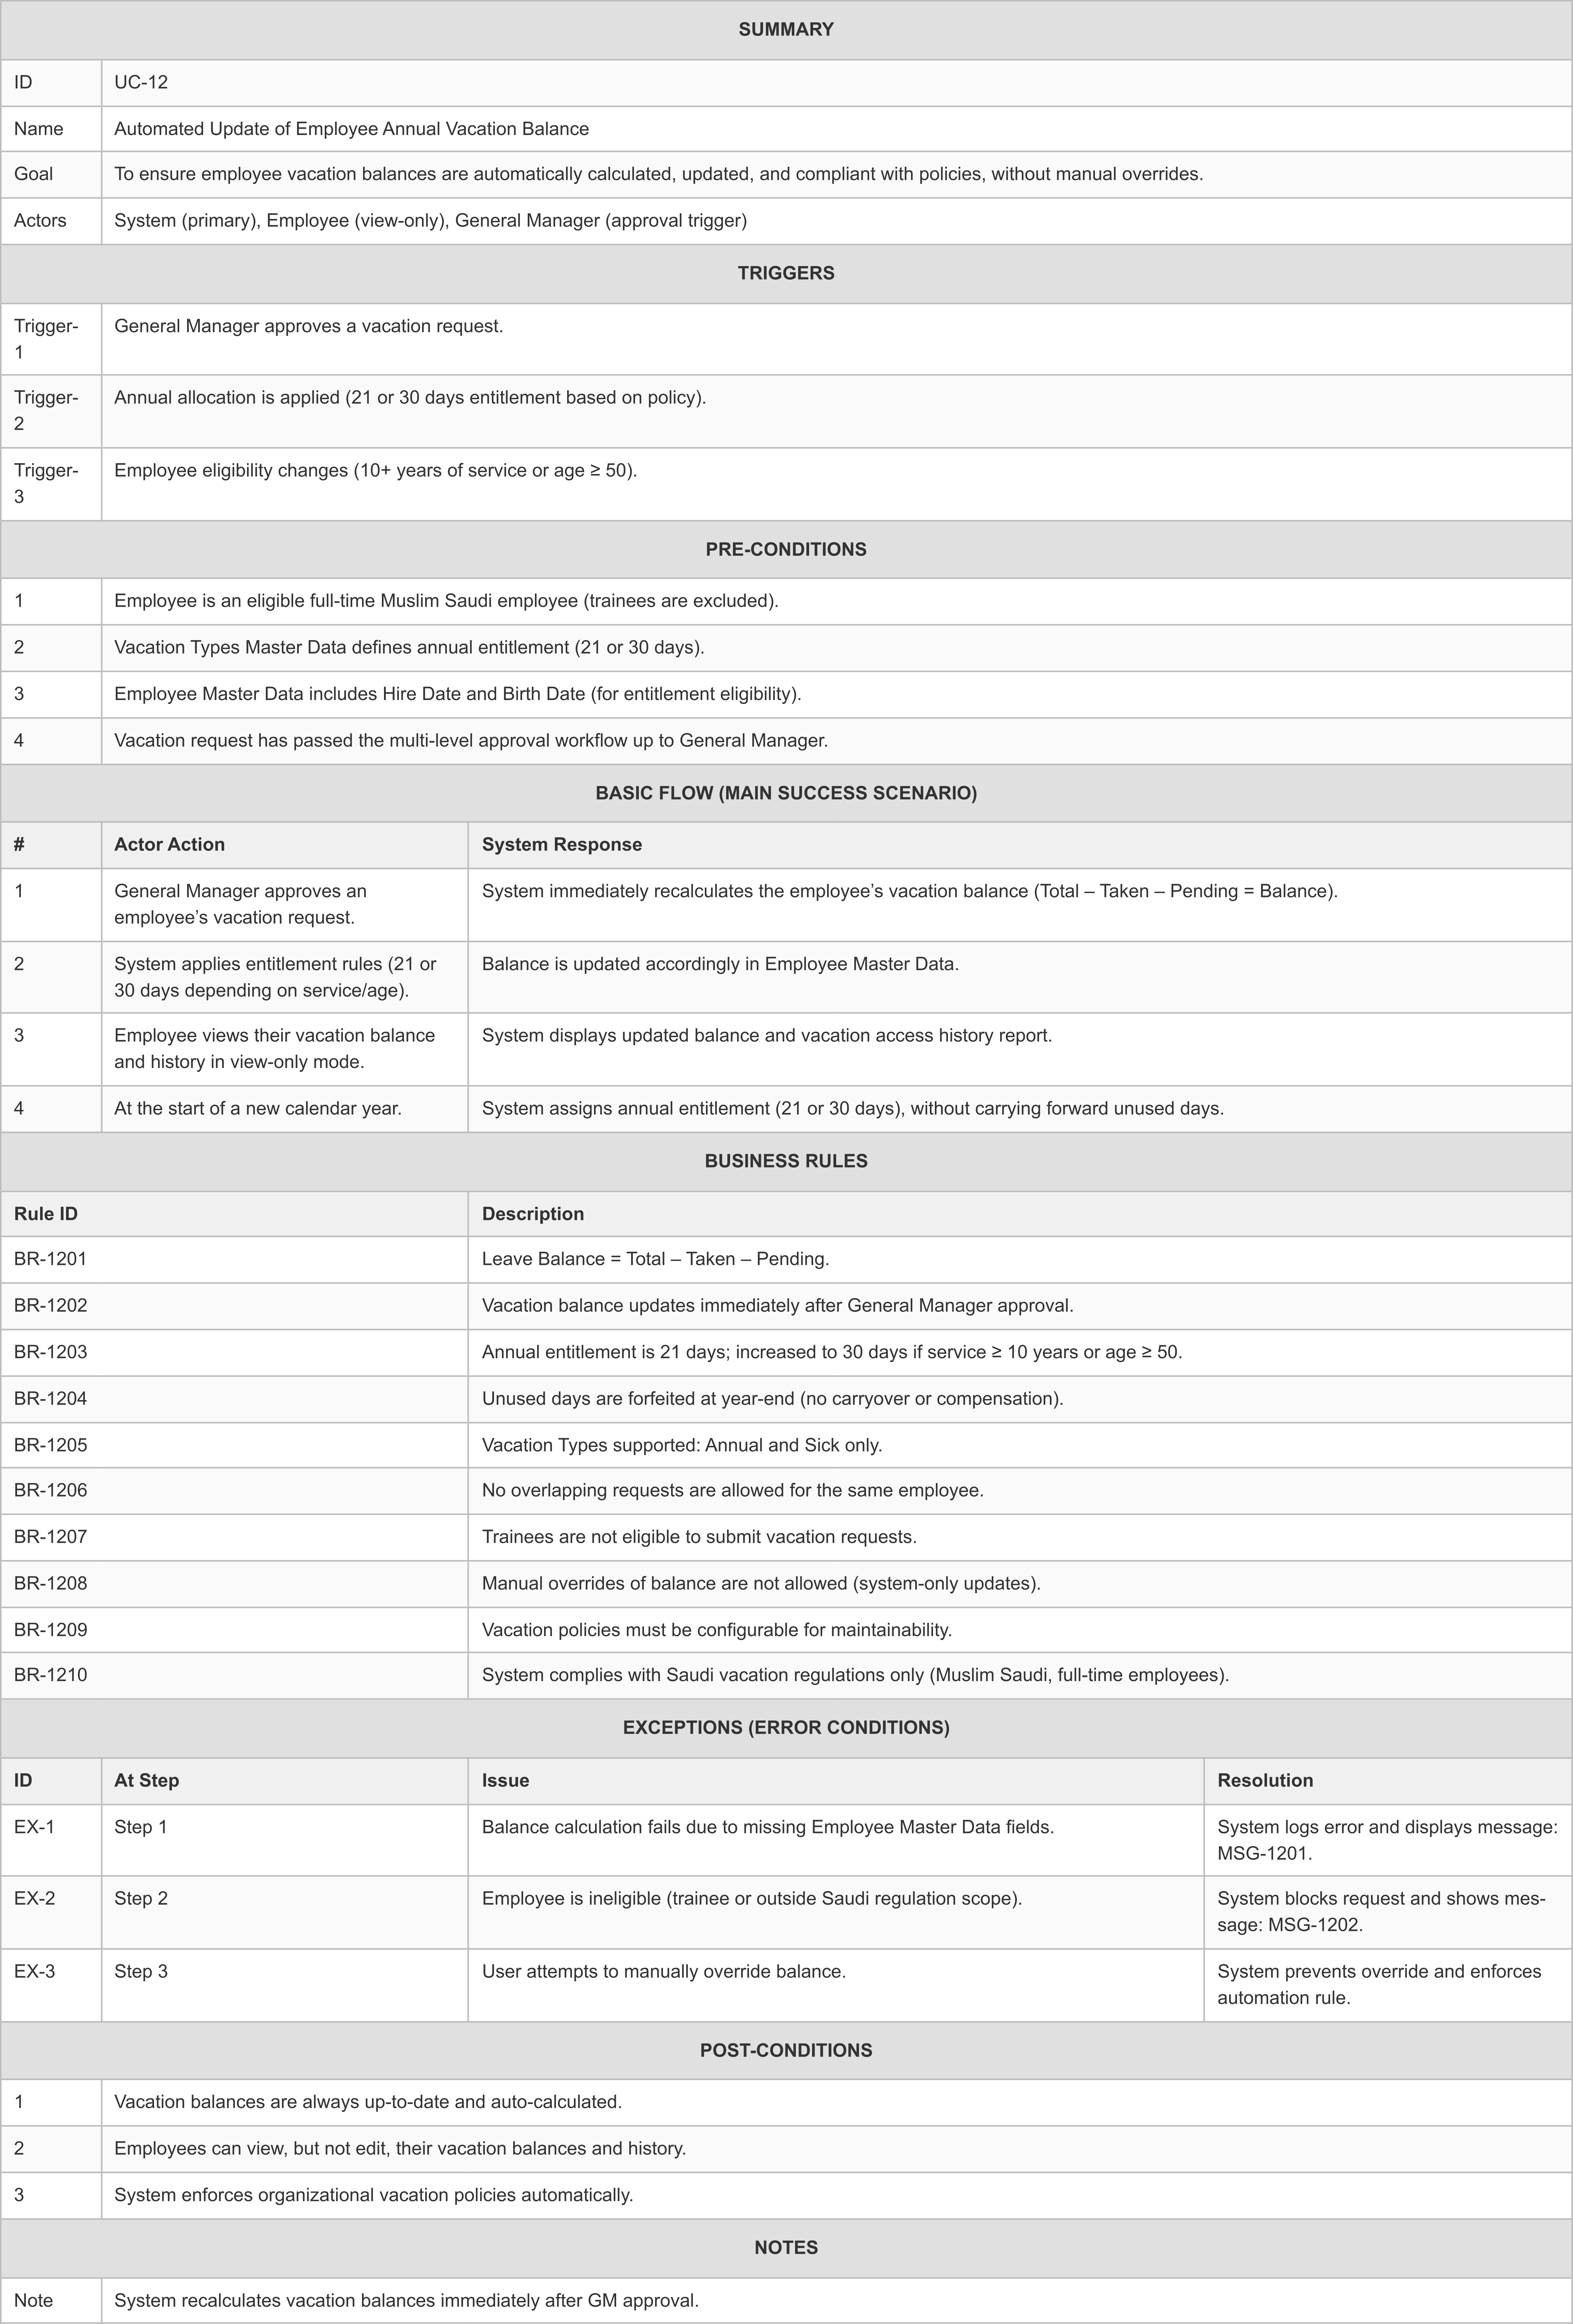
\includegraphics[width=0.9\textwidth]{Use-Cases/UC-12-Automated-Update-of-Employee-Annual-Vacation-Balance/UC-12-Automated-Update-of-Employee-Annual-Vacation-Balance-1.png}
\caption{UC-12: Automated Update of Employee Annual Vacation Balance Use Case}
\label{fig:uc12}
\end{figure}

\subsection{System Component Mapping and Traceability}
The following table provides a comprehensive mapping between use cases, business rules, functional requirements, user interfaces, and data entities to ensure complete traceability:

\begin{table}[H]
\centering
\begin{tabular}{|p{2cm}|p{2.5cm}|p{2.5cm}|p{2.5cm}|p{2.5cm}|}
\hline
\textbf{Use Case} & \textbf{Business Rules} & \textbf{Functional Requirements} & \textbf{User Interfaces} & \textbf{Data Entities} \\
\hline
UC-1 & BR-001, BR-002, BR-003, BR-011, BR-012, BR-013, BR-014 & FR-001 & Vacation Request Screen & Employee Master, Vacation Request, Vacation Types \\
\hline
UC-2 & BR-015, BR-016 & FR-002 & Vacation Cancellation Screen & Vacation Cancellation, Vacation Request \\
\hline
UC-3 & BR-015, BR-016 & FR-002 & My Vacation Requests Screen & Vacation Request, Vacation Cancellation \\
\hline
UC-4 & BR-006, BR-007, BR-008, BR-009, BR-014 & FR-003 & Review Vacation Request Screen & Vacation Request, Approval History \\
\hline
UC-5 & BR-015, BR-016, BR-009 & FR-003 & Review Cancellation Screen & Vacation Cancellation, Approval History \\
\hline
UC-6 & BR-006, BR-007 & FR-003 & Pending Requests Screen & Vacation Request, Approval History \\
\hline
UC-7 & BR-018 & FR-004 & Inquiry Search Parameters & Employee Master, Departments, Vacation Types \\
\hline
UC-8 & BR-018 & FR-004 & Inquiry Search Results & Vacation Request, Employee Master \\
\hline
UC-9 & BR-018 & FR-005 & Single Transaction Report & Vacation Request, Employee Master, Approval History \\
\hline
UC-10 & BR-018 & FR-005 & Comparative Report & Employee Master, Departments, Vacation Request \\
\hline
UC-11 & BR-017 & FR-007 & Notifications Center & Notification Data \\
\hline
UC-12 & BR-001, BR-002, BR-008, BR-019 & FR-006 & System Process & Employee Master, Vacation Request \\
\hline
\end{tabular}
\caption{Comprehensive System Component Mapping and Traceability Matrix}
\end{table}

This mapping ensures that:
\begin{itemize}
    \item Each use case is supported by appropriate business rules
    \item Functional requirements are derived from use cases
    \item User interfaces are designed for specific use cases
    \item Data entities support all system operations
    \item Complete traceability is maintained throughout the system
\end{itemize}

\section{Functional Requirements}

This section describes the system's functional requirements derived from use cases, focusing on what the system must do rather than how it does it.

\subsection{FR-001: Vacation Request Management}
\textbf{Description}: The system must allow employees to create and submit vacation requests.
\textbf{Inputs}: Start date, end date, vacation type, notes, attachments
\textbf{Processing}: Validate dates, check balance, calculate period, prevent overlaps
\textbf{Outputs}: Request ID, confirmation message, workflow initiation
\textbf{Business Rules}: BR-001, BR-002, BR-003, BR-011, BR-012, BR-013, BR-014
\textbf{Use Cases}: UC-1

\subsection{FR-002: Vacation Cancellation Management}
\textbf{Description}: The system must allow employees to cancel pending or approved vacation requests.
\textbf{Inputs}: Cancellation reason, original request reference
\textbf{Processing}: Validate cancellation eligibility, create cancellation request
\textbf{Outputs}: Cancellation request ID, approval workflow initiation
\textbf{Business Rules}: BR-015, BR-016
\textbf{Use Cases}: UC-2, UC-3

\subsection{FR-003: Multi-Level Approval Workflow}
\textbf{Description}: The system must implement a four-level approval process with automatic escalation.
\textbf{Inputs}: Manager decisions, reasons, approval levels
\textbf{Processing}: Route through approval hierarchy, track decisions, escalate delays
\textbf{Outputs}: Approval status updates, notifications, workflow progression
\textbf{Business Rules}: BR-006, BR-007, BR-008, BR-009
\textbf{Use Cases}: UC-4, UC-6

\subsection{FR-004: Vacation Inquiry and Search}
\textbf{Description}: The system must provide comprehensive search and inquiry capabilities.
\textbf{Inputs}: Search criteria (dates, department, employee, type, status)
\textbf{Processing}: Apply filters, execute search, paginate results
\textbf{Outputs}: Filtered results grid, export options, pagination controls
\textbf{Business Rules}: BR-018
\textbf{Use Cases}: UC-7, UC-8

\subsection{FR-005: Report Generation}
\textbf{Description}: The system must generate PDF reports for vacation data.
\textbf{Inputs}: Report parameters, data selection, format preferences
\textbf{Processing}: Format data, generate PDF, include standard footer
\textbf{Outputs}: PDF report with complete details and footer information
\textbf{Business Rules}: BR-018
\textbf{Use Cases}: UC-9, UC-10

\subsection{FR-006: Automated Balance Management}
\textbf{Description}: The system must automatically calculate and update employee vacation balances.
\textbf{Inputs}: Approval triggers, entitlement rules, usage data
\textbf{Processing}: Calculate balance, apply entitlement rules, update records
\textbf{Outputs}: Updated vacation balances, audit trail
\textbf{Business Rules}: BR-001, BR-002, BR-008, BR-019
\textbf{Use Cases}: UC-12

\subsection{FR-007: Notification System}
\textbf{Description}: The system must provide real-time notifications for all stakeholders.
\textbf{Inputs}: System events, user preferences, notification types
\textbf{Processing}: Generate notifications, deliver to users, track delivery
\textbf{Outputs}: User notifications, delivery confirmations
\textbf{Business Rules}: BR-017
\textbf{Use Cases}: UC-11

\section{Non-Functional Requirements}

\subsection{Performance Requirements}

\subsubsection{NFR-001: Response Time}
\textbf{Requirement}: Page load must complete within 3 seconds from user click to interactive display.
\textbf{Measurement}: Time from HTTP request initiation to page render completion.
\textbf{Applicable Use Cases}: All user interface interactions.

\subsubsection{NFR-002: Throughput}
\textbf{Requirement}: System must support 100+ concurrent users without performance degradation.
\textbf{Measurement}: Response time remains under 3 seconds with 100 simultaneous users.
\textbf{Applicable Use Cases}: All system functions.

\subsubsection{NFR-003: Availability}
\textbf{Requirement}: System must maintain 99.5\% uptime during business hours (8 AM - 6 PM, Sunday-Thursday).
\textbf{Measurement}: Monthly uptime calculation excluding scheduled maintenance.
\textbf{Applicable Use Cases}: All system functions.

\subsubsection{NFR-004: Scalability}
\textbf{Requirement}: System must support up to 1000 employees without architectural changes.
\textbf{Measurement}: Performance metrics remain within acceptable ranges at maximum capacity.
\textbf{Applicable Use Cases}: All system functions.

\subsubsection{NFR-005: PDF Generation}
\textbf{Requirement}: PDF report generation must complete within 5 seconds for standard reports.
\textbf{Measurement}: Time from report request to PDF download availability.
\textbf{Applicable Use Cases}: UC-9, UC-10.

\subsection{Security Requirements}

\subsubsection{NFR-006: Authentication}
\textbf{Requirement}: System must implement secure login with session management.
\textbf{Implementation}: Multi-factor authentication, session timeout after 30 minutes of inactivity.
\textbf{Applicable Use Cases}: All system access.

\subsubsection{NFR-007: Authorization}
\textbf{Requirement}: System must implement role-based access control.
\textbf{Implementation}: User permissions based on organizational role and hierarchy.
\textbf{Applicable Use Cases}: All system functions.

\subsubsection{NFR-008: Data Protection}
\textbf{Requirement}: System must encrypt sensitive employee information.
\textbf{Implementation}: AES-256 encryption for data at rest and in transit.
\textbf{Applicable Use Cases}: All data handling functions.

\subsubsection{NFR-009: Audit Trail}
\textbf{Requirement}: System must log all activities for audit purposes.
\textbf{Implementation}: Comprehensive logging of user actions, system events, and data changes.
\textbf{Applicable Use Cases}: All system functions.

\subsubsection{NFR-010: Input Validation}
\textbf{Requirement}: System must prevent SQL injection and XSS attacks.
\textbf{Implementation}: Input sanitization, parameterized queries, output encoding.
\textbf{Applicable Use Cases}: All user input functions.

\subsection{Usability Requirements}

\subsubsection{NFR-011: User Interface}
\textbf{Requirement}: System must provide intuitive, responsive design.
\textbf{Implementation}: Modern web standards, consistent navigation, clear visual hierarchy.
\textbf{Applicable Use Cases}: All user interface interactions.

\subsubsection{NFR-012: Accessibility}
\textbf{Requirement}: System must comply with WCAG 2.1 AA standards.
\textbf{Implementation}: Screen reader support, keyboard navigation, color contrast compliance.
\textbf{Applicable Use Cases}: All user interface interactions.

\subsubsection{NFR-013: Multi-language Support}
\textbf{Requirement}: System must support Arabic and English languages.
\textbf{Implementation}: Localized interface, right-to-left text support, cultural adaptations.
\textbf{Applicable Use Cases}: All user interface interactions.

\subsubsection{NFR-014: Mobile Support}
\textbf{Requirement}: System must provide responsive design for all devices.
\textbf{Implementation}: Mobile-first design, touch-friendly interfaces, adaptive layouts.
\textbf{Applicable Use Cases}: All user interface interactions.

\subsubsection{NFR-015: Error Handling}
\textbf{Requirement}: System must provide clear, actionable error messages.
\textbf{Implementation}: User-friendly error descriptions with specific resolution steps.
\textbf{Applicable Use Cases}: All system functions.

\subsection{Reliability Requirements}

\subsubsection{NFR-016: Error Handling}
\textbf{Requirement}: System must handle errors gracefully without data loss.
\textbf{Implementation}: Comprehensive error catching, user notification, automatic recovery where possible.
\textbf{Applicable Use Cases}: All system functions.

\subsubsection{NFR-017: Data Integrity}
\textbf{Requirement}: System must prevent data corruption and maintain consistency.
\textbf{Implementation}: Transaction management, referential integrity, validation checks.
\textbf{Applicable Use Cases}: All data operations.

\subsubsection{NFR-018: Backup and Recovery}
\textbf{Requirement}: System must provide daily automated backups with 4-hour maximum recovery time.
\textbf{Implementation}: Automated backup scheduling, point-in-time recovery capability.
\textbf{Applicable Use Cases}: All system functions.

\subsubsection{NFR-019: Validation}
\textbf{Requirement}: System must implement comprehensive business rule validation.
\textbf{Implementation}: Real-time validation, business rule enforcement, error prevention.
\textbf{Applicable Use Cases}: All data input functions.

\section{User Interface Overview}

This section provides the system's user interface wireframes and visual specifications.

\subsection{Core Application Screens}

\subsubsection{Vacation Request Screen}
\begin{figure}[H]
\centering
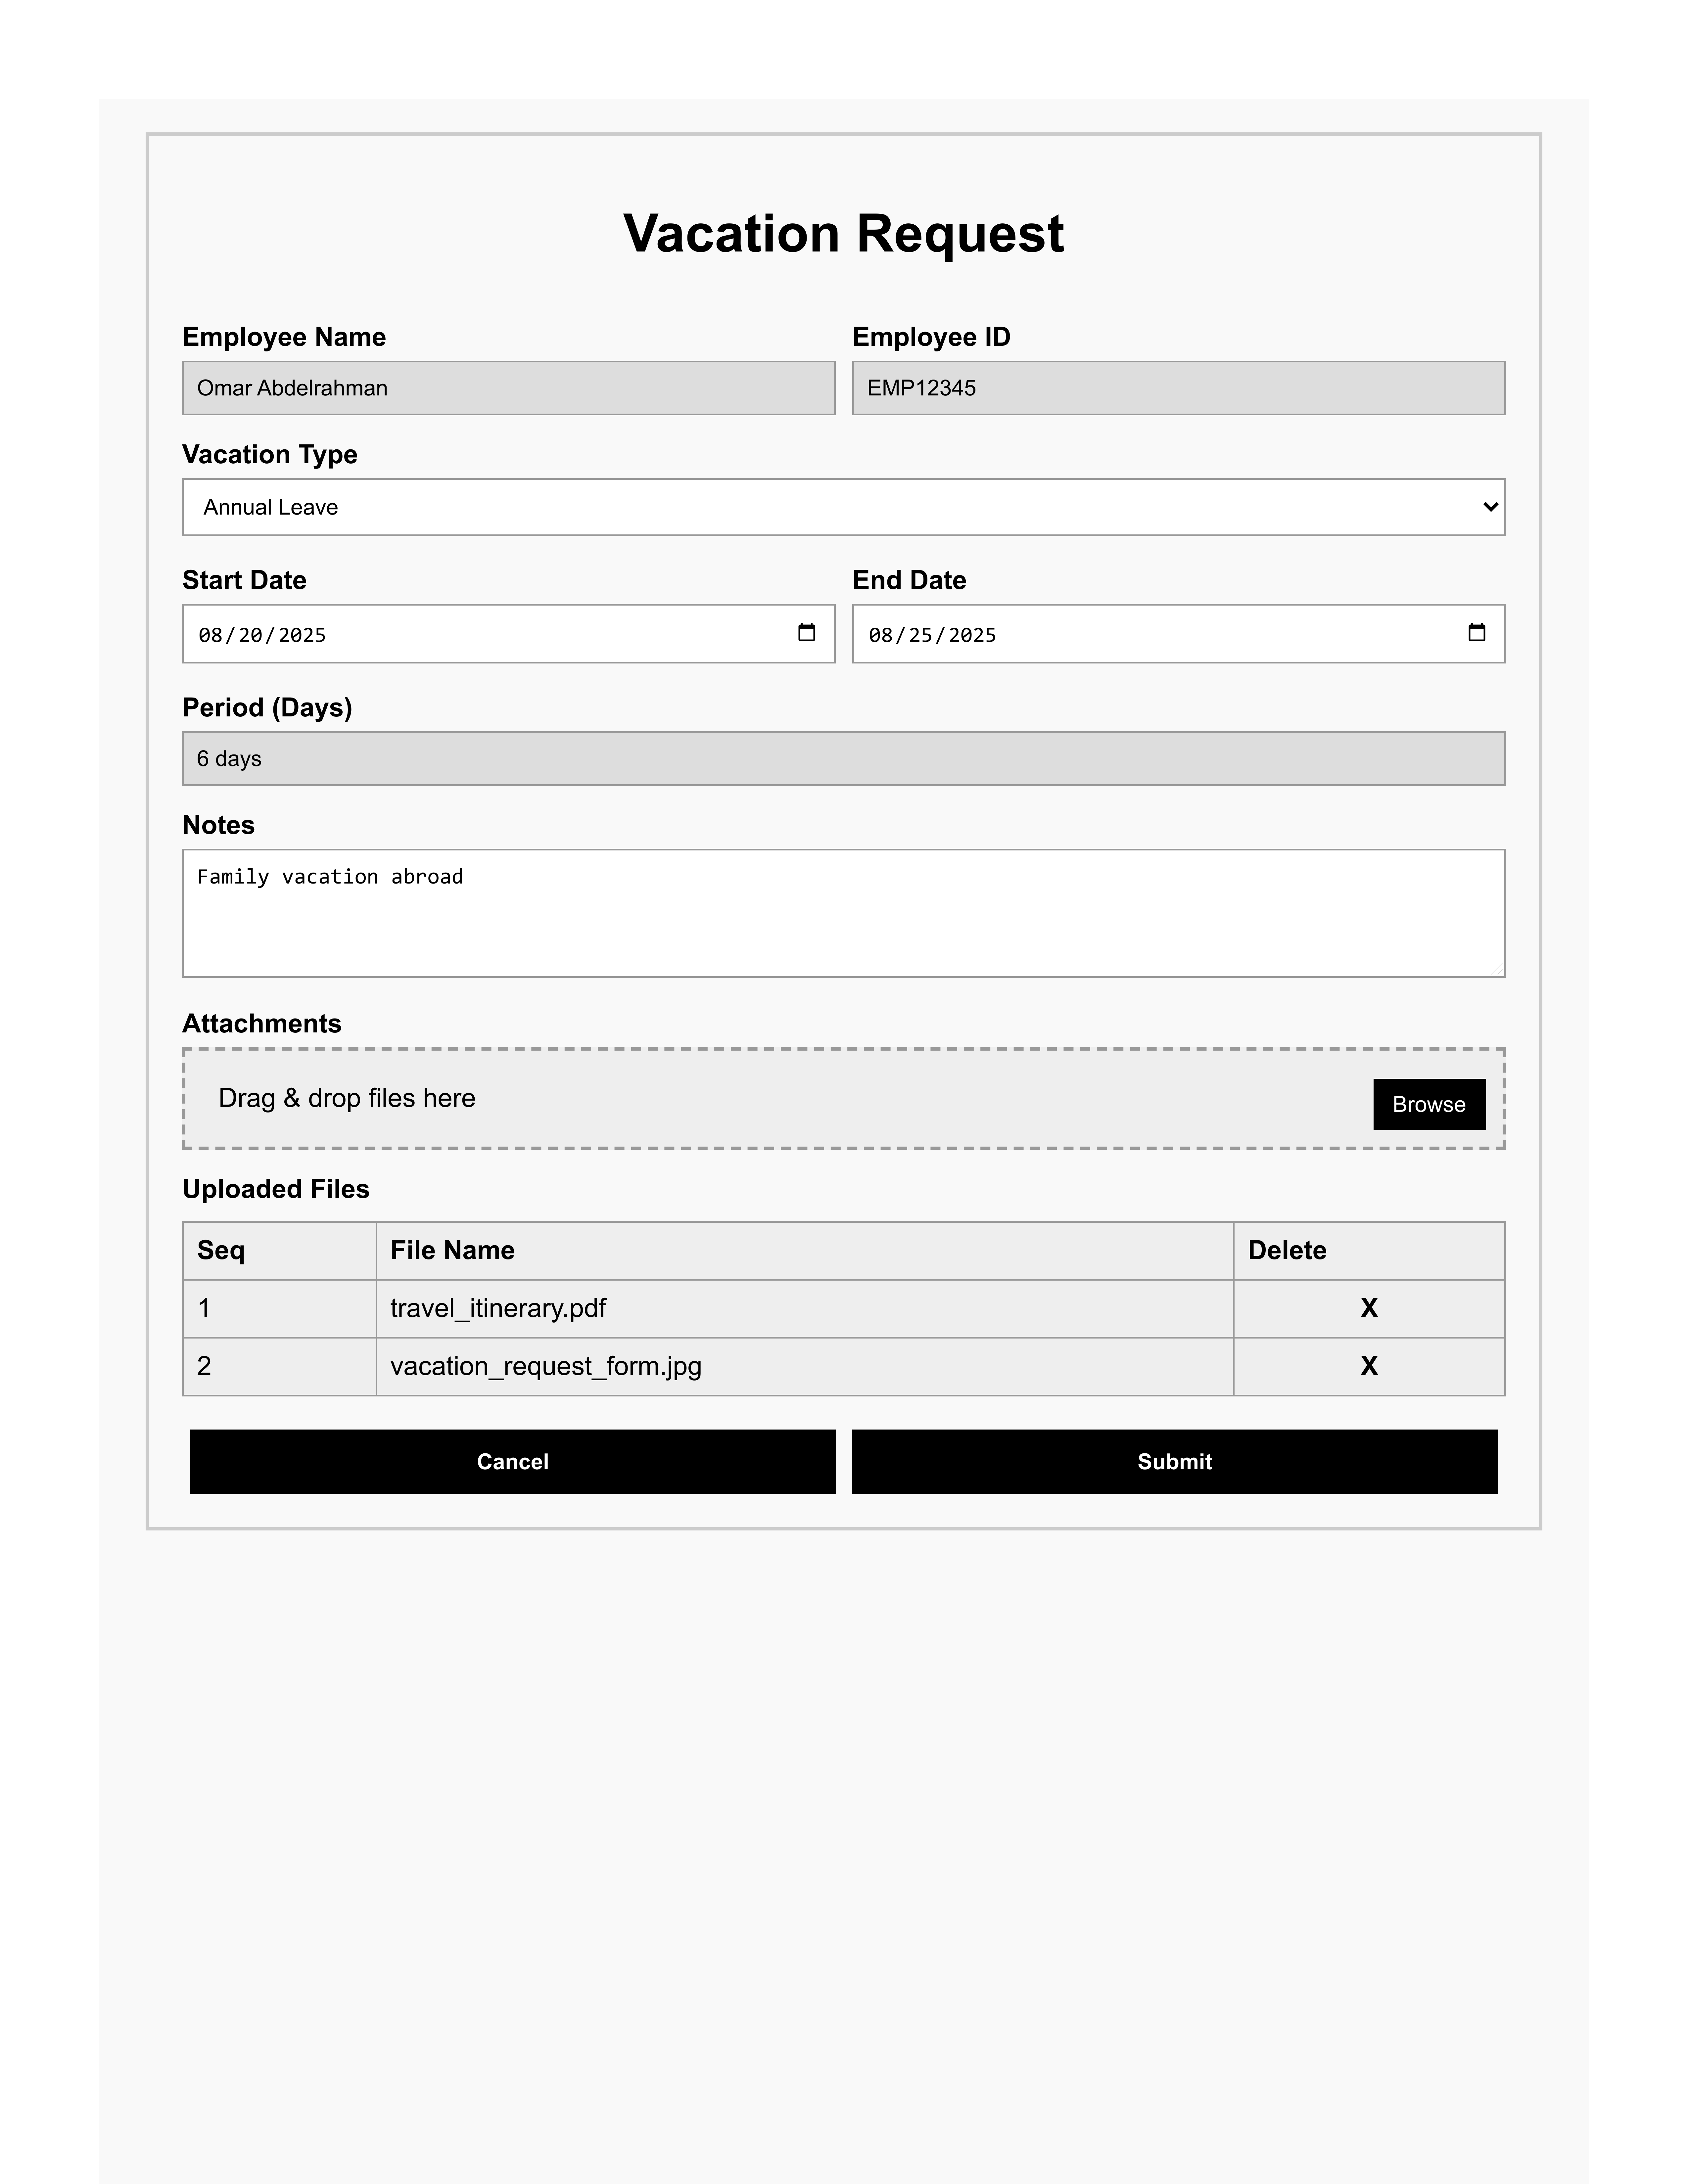
\includegraphics[width=0.9\textwidth]{Wireframes/Vacation-Request/Vacation-Request-1.png}
\caption{Vacation Request Screen}
\label{fig:vacation-request-screen}
\end{figure}

\subsubsection{Vacation Cancellation Request Screen}
\begin{figure}[H]
\centering
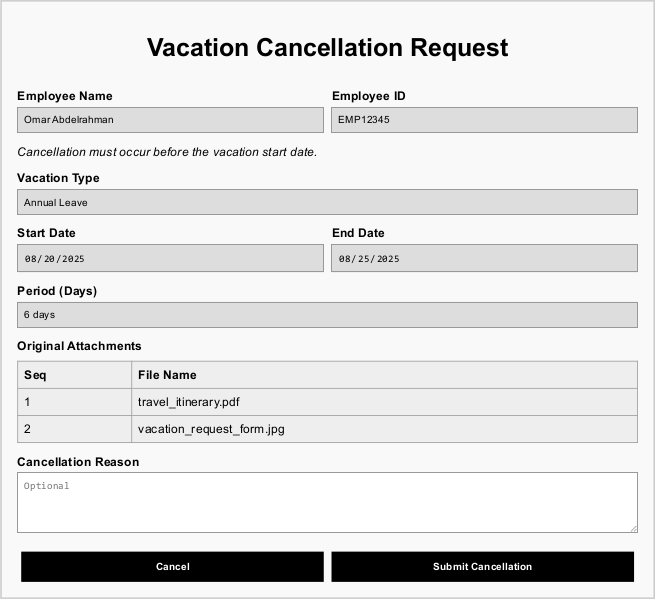
\includegraphics[width=0.9\textwidth]{Wireframes/Vacation-Cancellation-Request/Vacation-Cancellation-Request-1.png}
\caption{Vacation Cancellation Request Screen}
\label{fig:vacation-cancellation-screen}
\end{figure}

\subsubsection{Review Vacation Request Screen}
\begin{figure}[H]
\centering
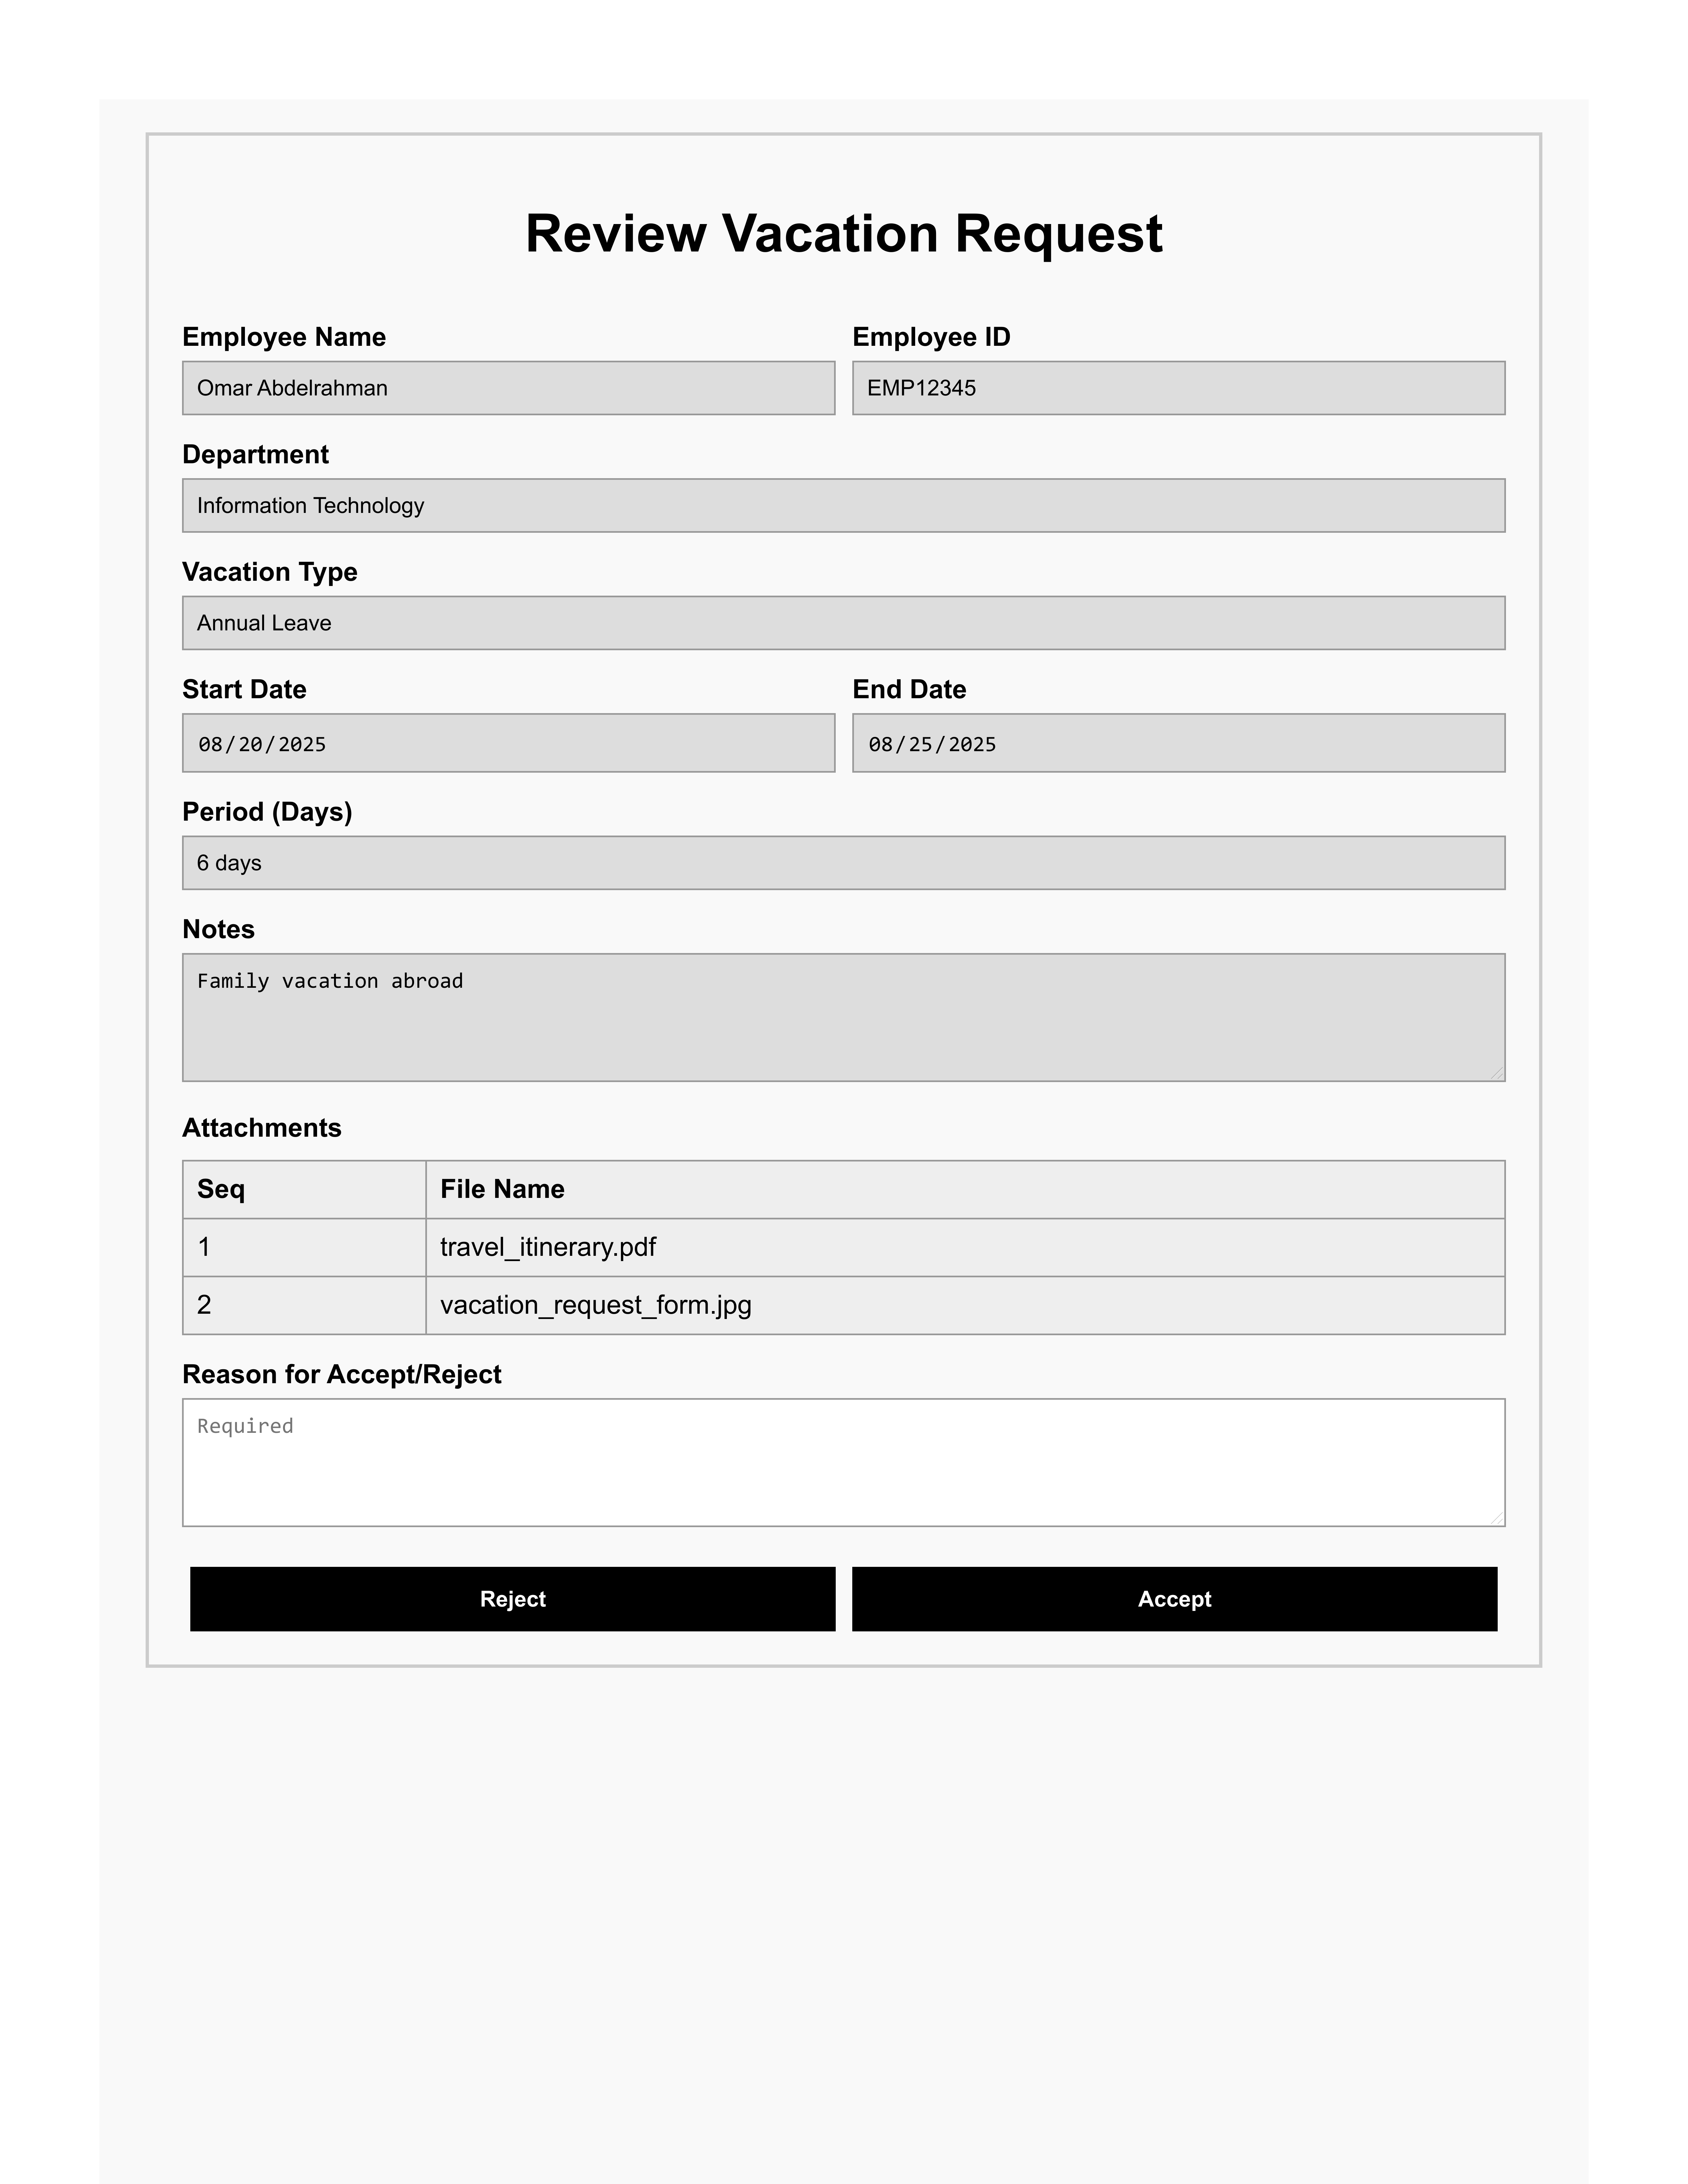
\includegraphics[width=0.9\textwidth]{Wireframes/Review-Vacation-Request/Review-Vacation-Request-1.png}
\caption{Review Vacation Request Screen}
\label{fig:review-vacation-screen}
\end{figure}

\subsubsection{Review Vacation Cancellation Request Screen}
\begin{figure}[H]
\centering
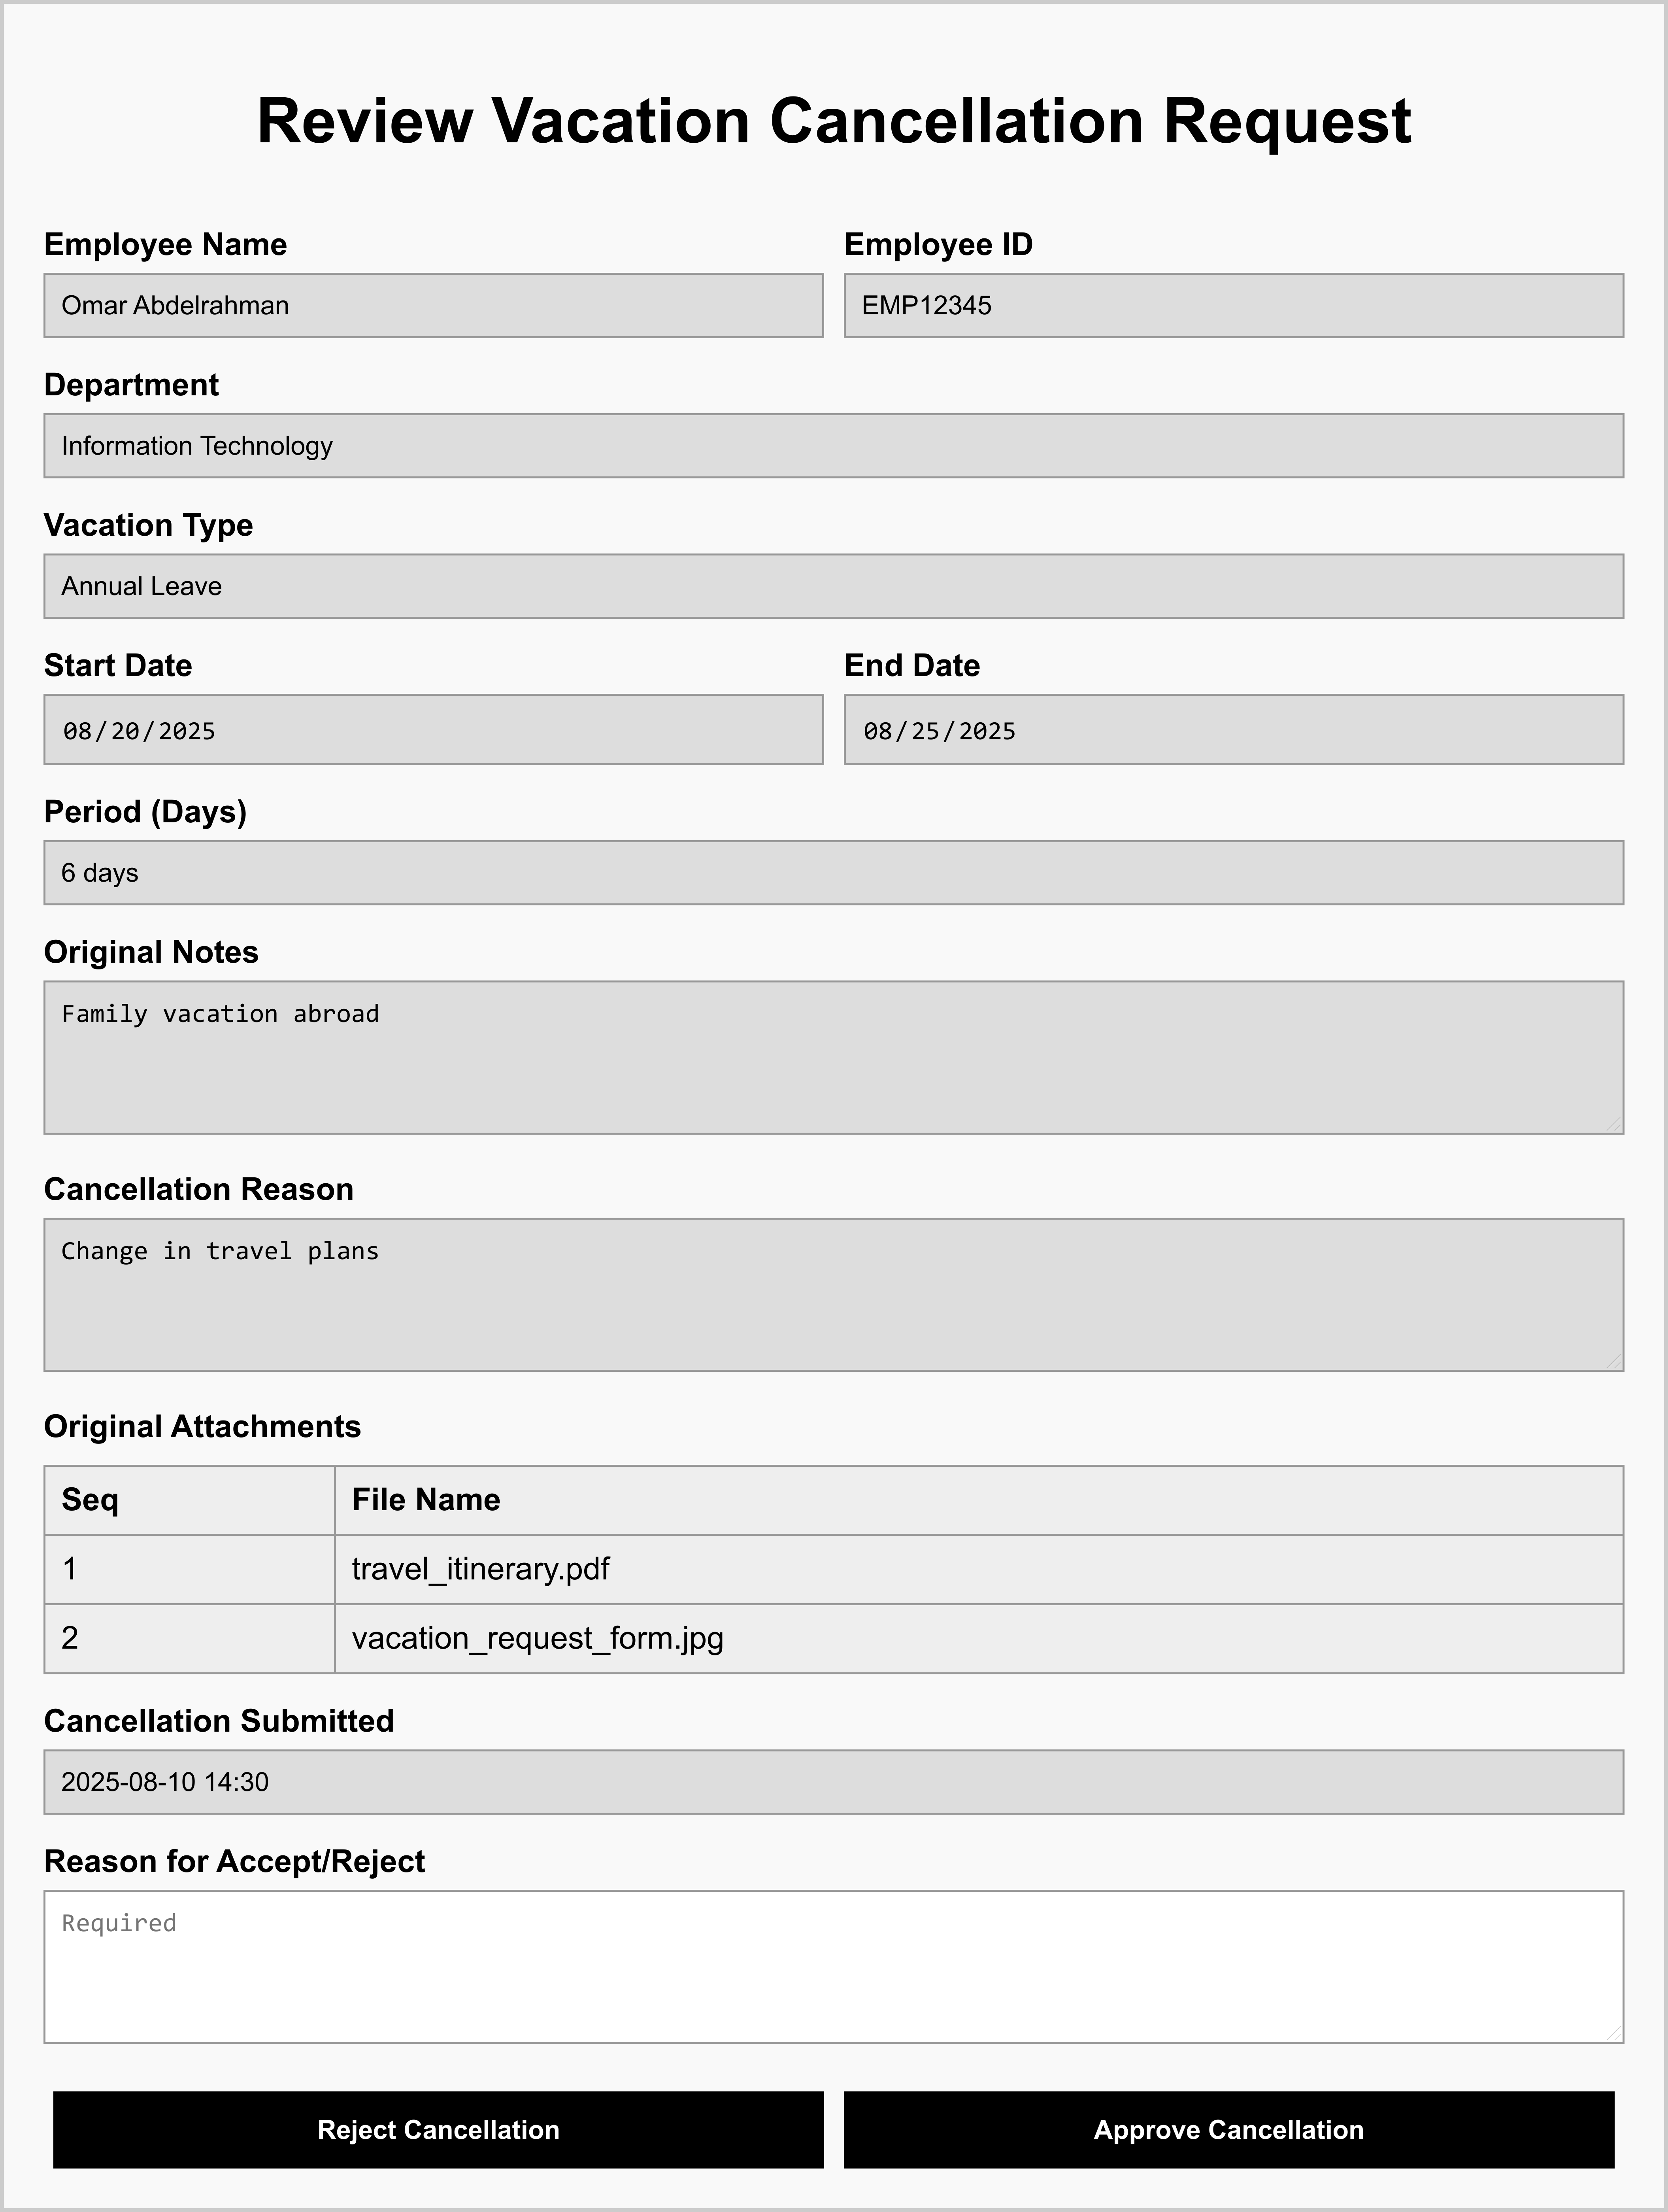
\includegraphics[width=0.9\textwidth]{Wireframes/Review-Vacation-Cancellation-Request/Review-Vacation-Cancellation-Request-1.png}
\caption{Review Vacation Cancellation Request Screen}
\label{fig:review-cancellation-screen}
\end{figure}

\subsubsection{My Vacation Requests Screen}
\begin{figure}[H]
\centering
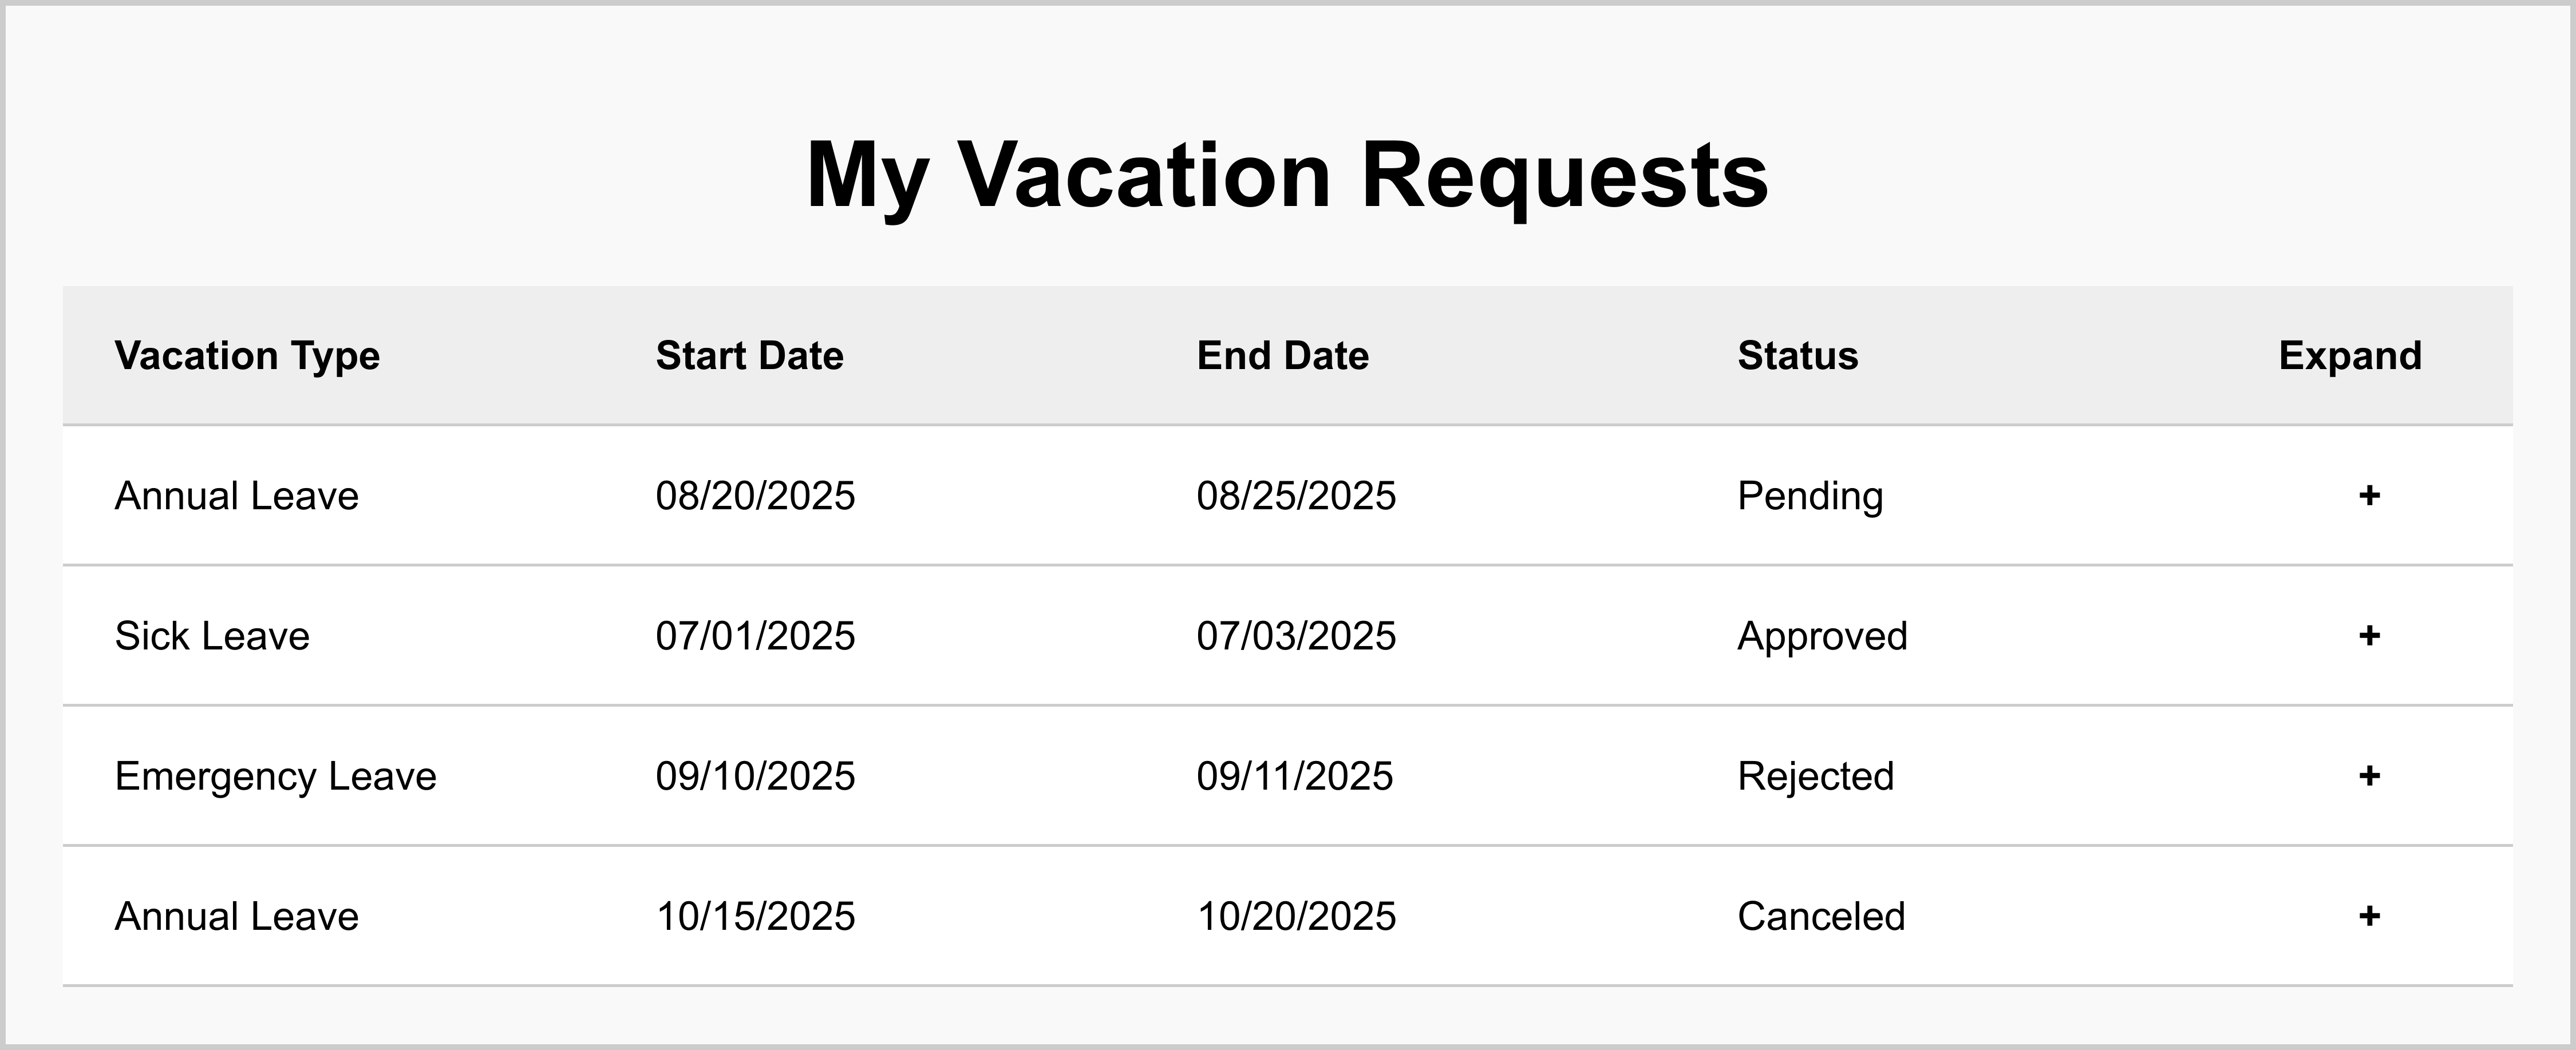
\includegraphics[width=0.9\textwidth]{Wireframes/My-Vacation-Requests/My-Vacation-Requests-1.png}
\caption{My Vacation Requests Screen}
\label{fig:my-vacation-requests-screen}
\end{figure}

\subsubsection{Pending Vacation Requests Screen}
\begin{figure}[H]
\centering
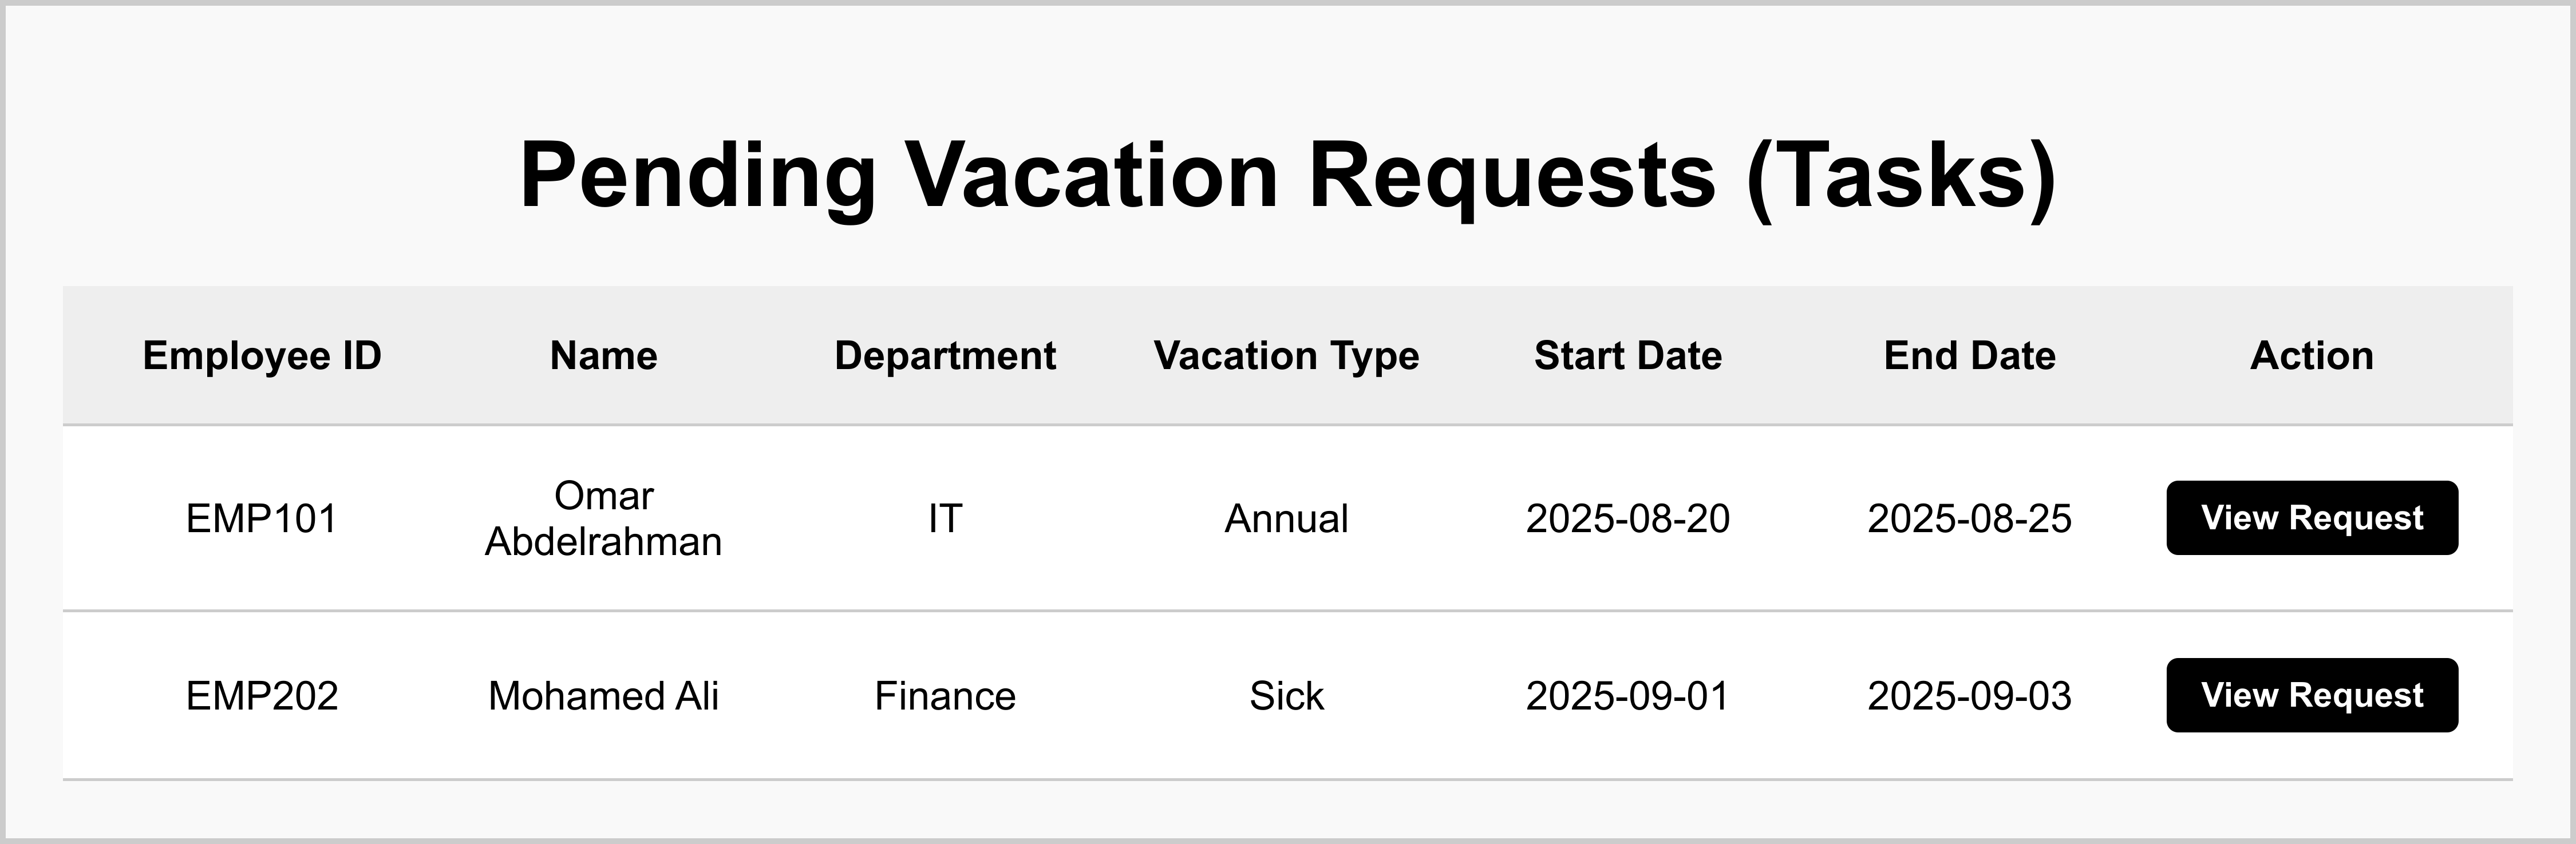
\includegraphics[width=0.9\textwidth]{Wireframes/Pending-Vacation-Requests/Pending-Vacation-Requests-1.png}
\caption{Pending Vacation Requests Screen}
\label{fig:pending-vacation-requests-screen}
\end{figure}

\subsubsection{Vacation Inquiry Search Parameters Screen}
\begin{figure}[H]
\centering
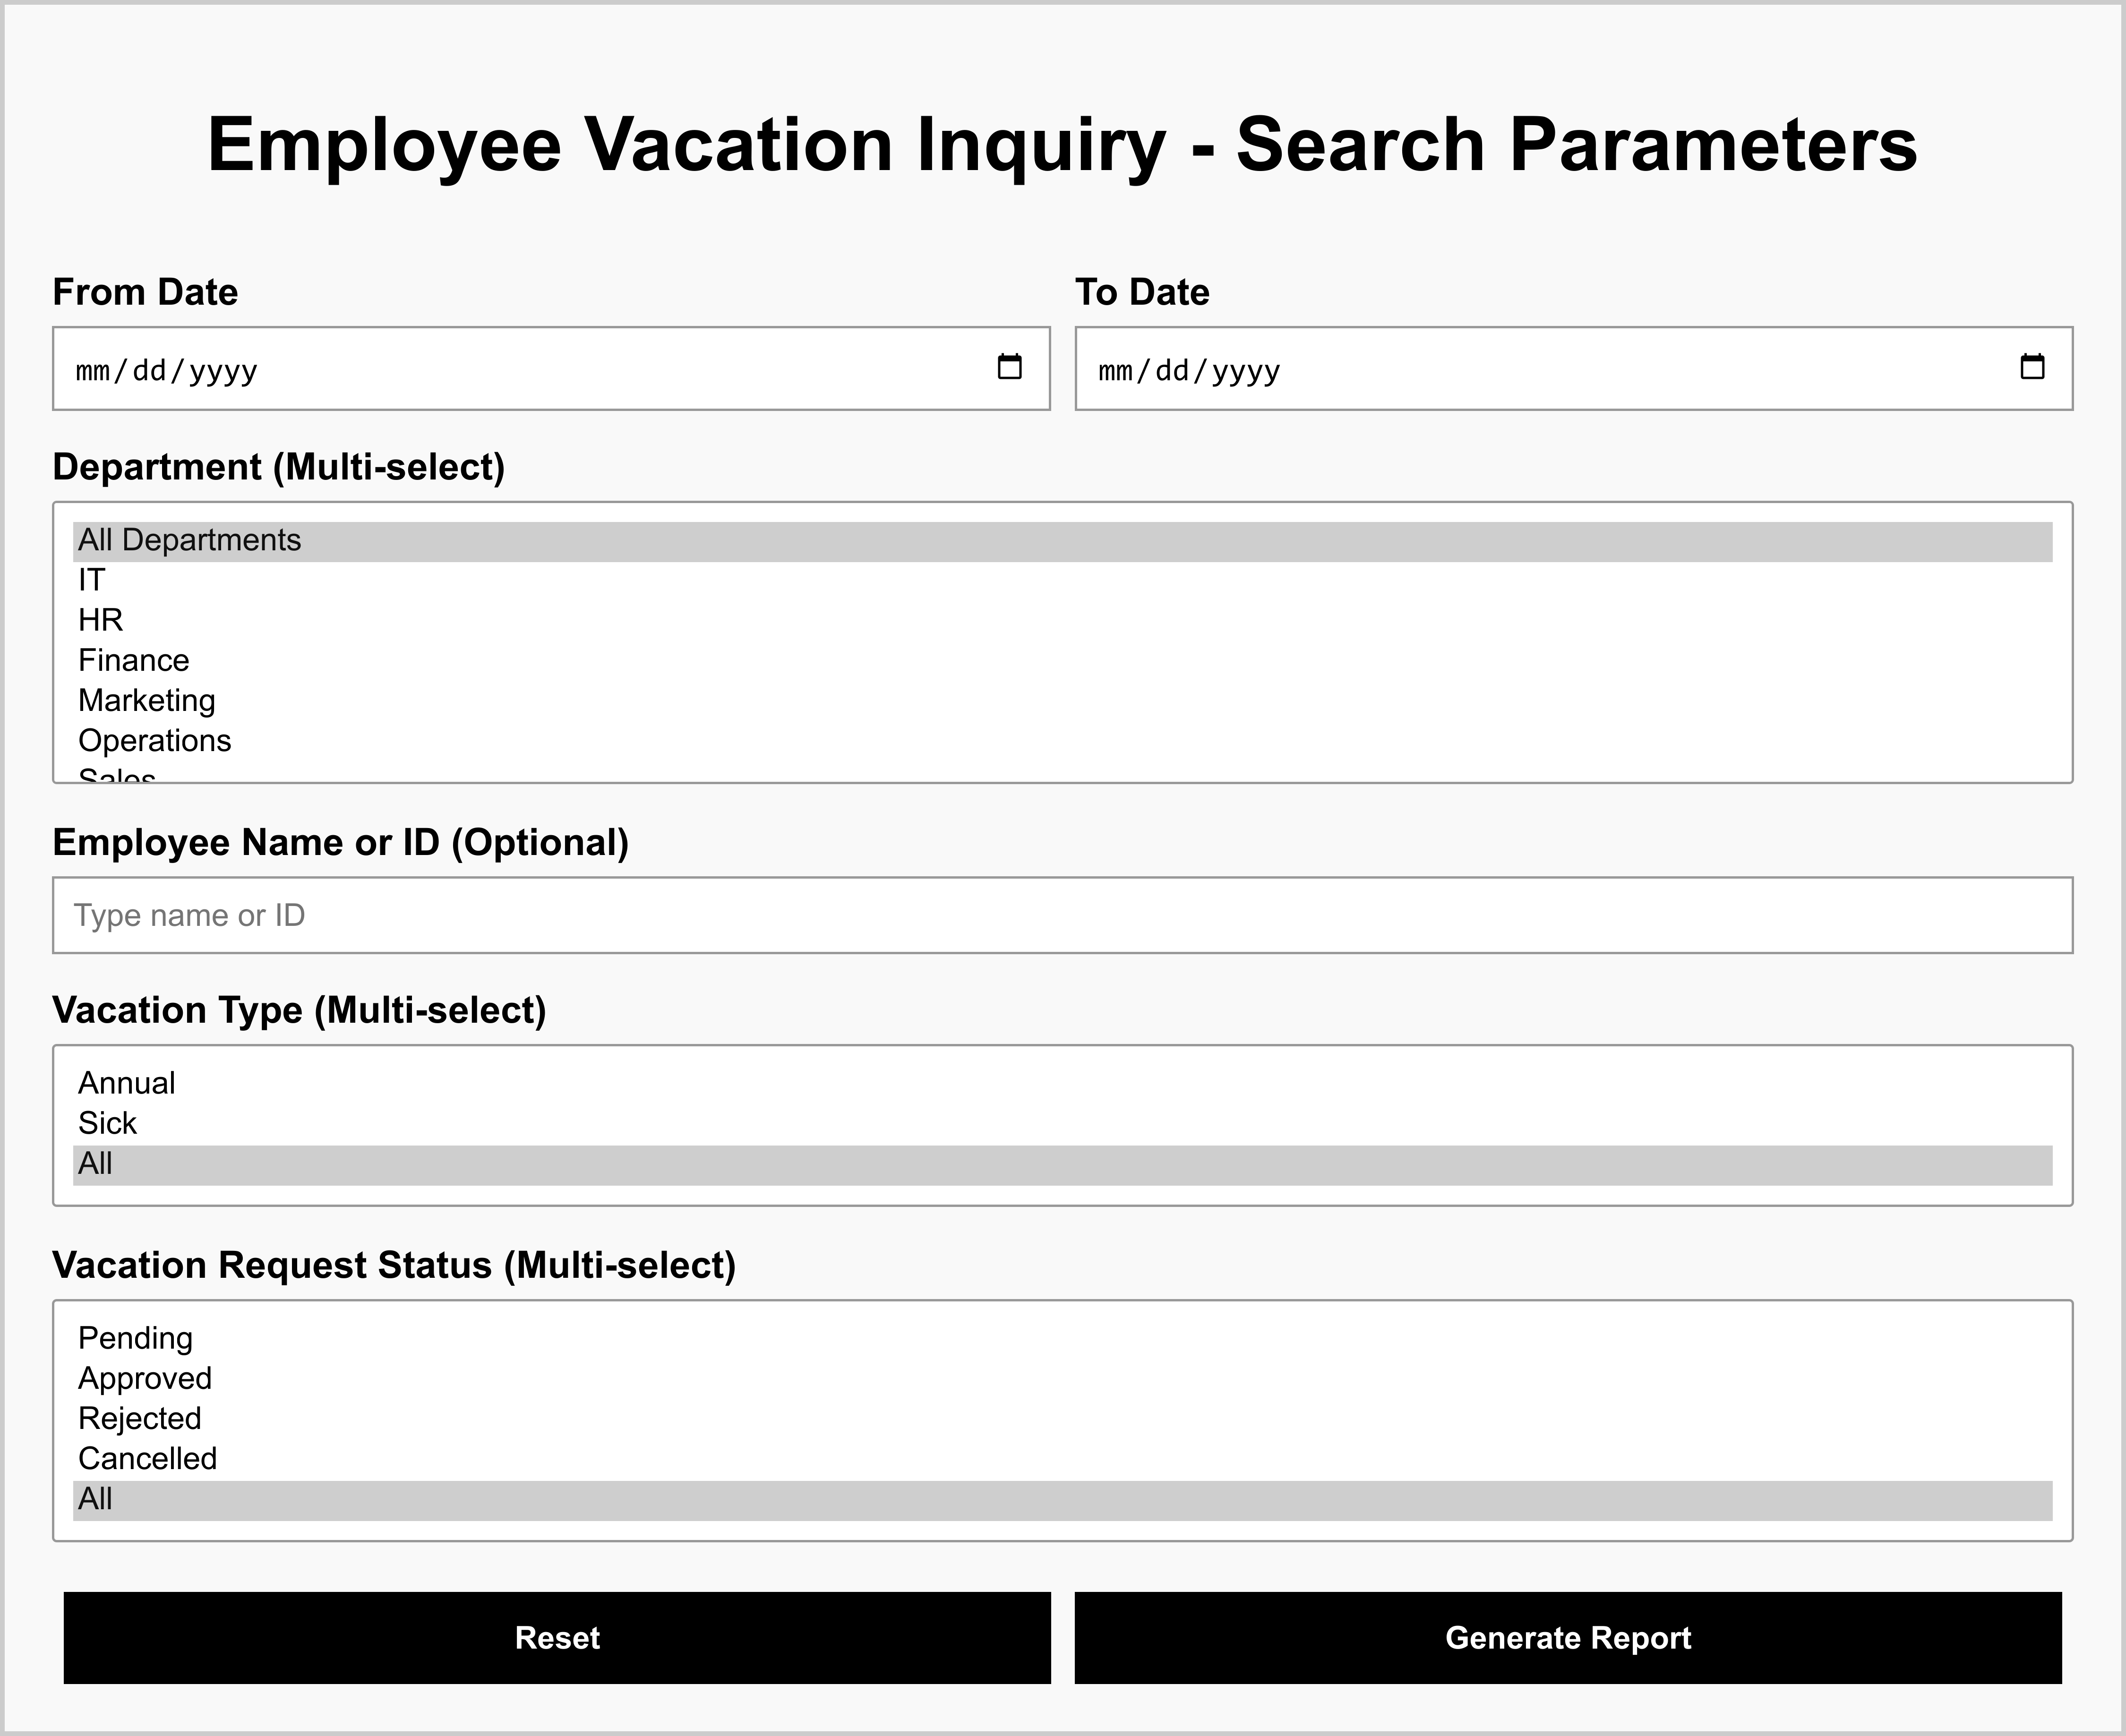
\includegraphics[width=0.9\textwidth]{Wireframes/Employee-Vacation-Inquiry-Search-Parameters/Employee-Vacation-Inquiry-Search-Parameters-1.png}
\caption{Vacation Inquiry Search Parameters Screen}
\label{fig:inquiry-search-params-screen}
\end{figure}

\subsubsection{Vacation Inquiry Search Results Screen}
\begin{figure}[H]
\centering
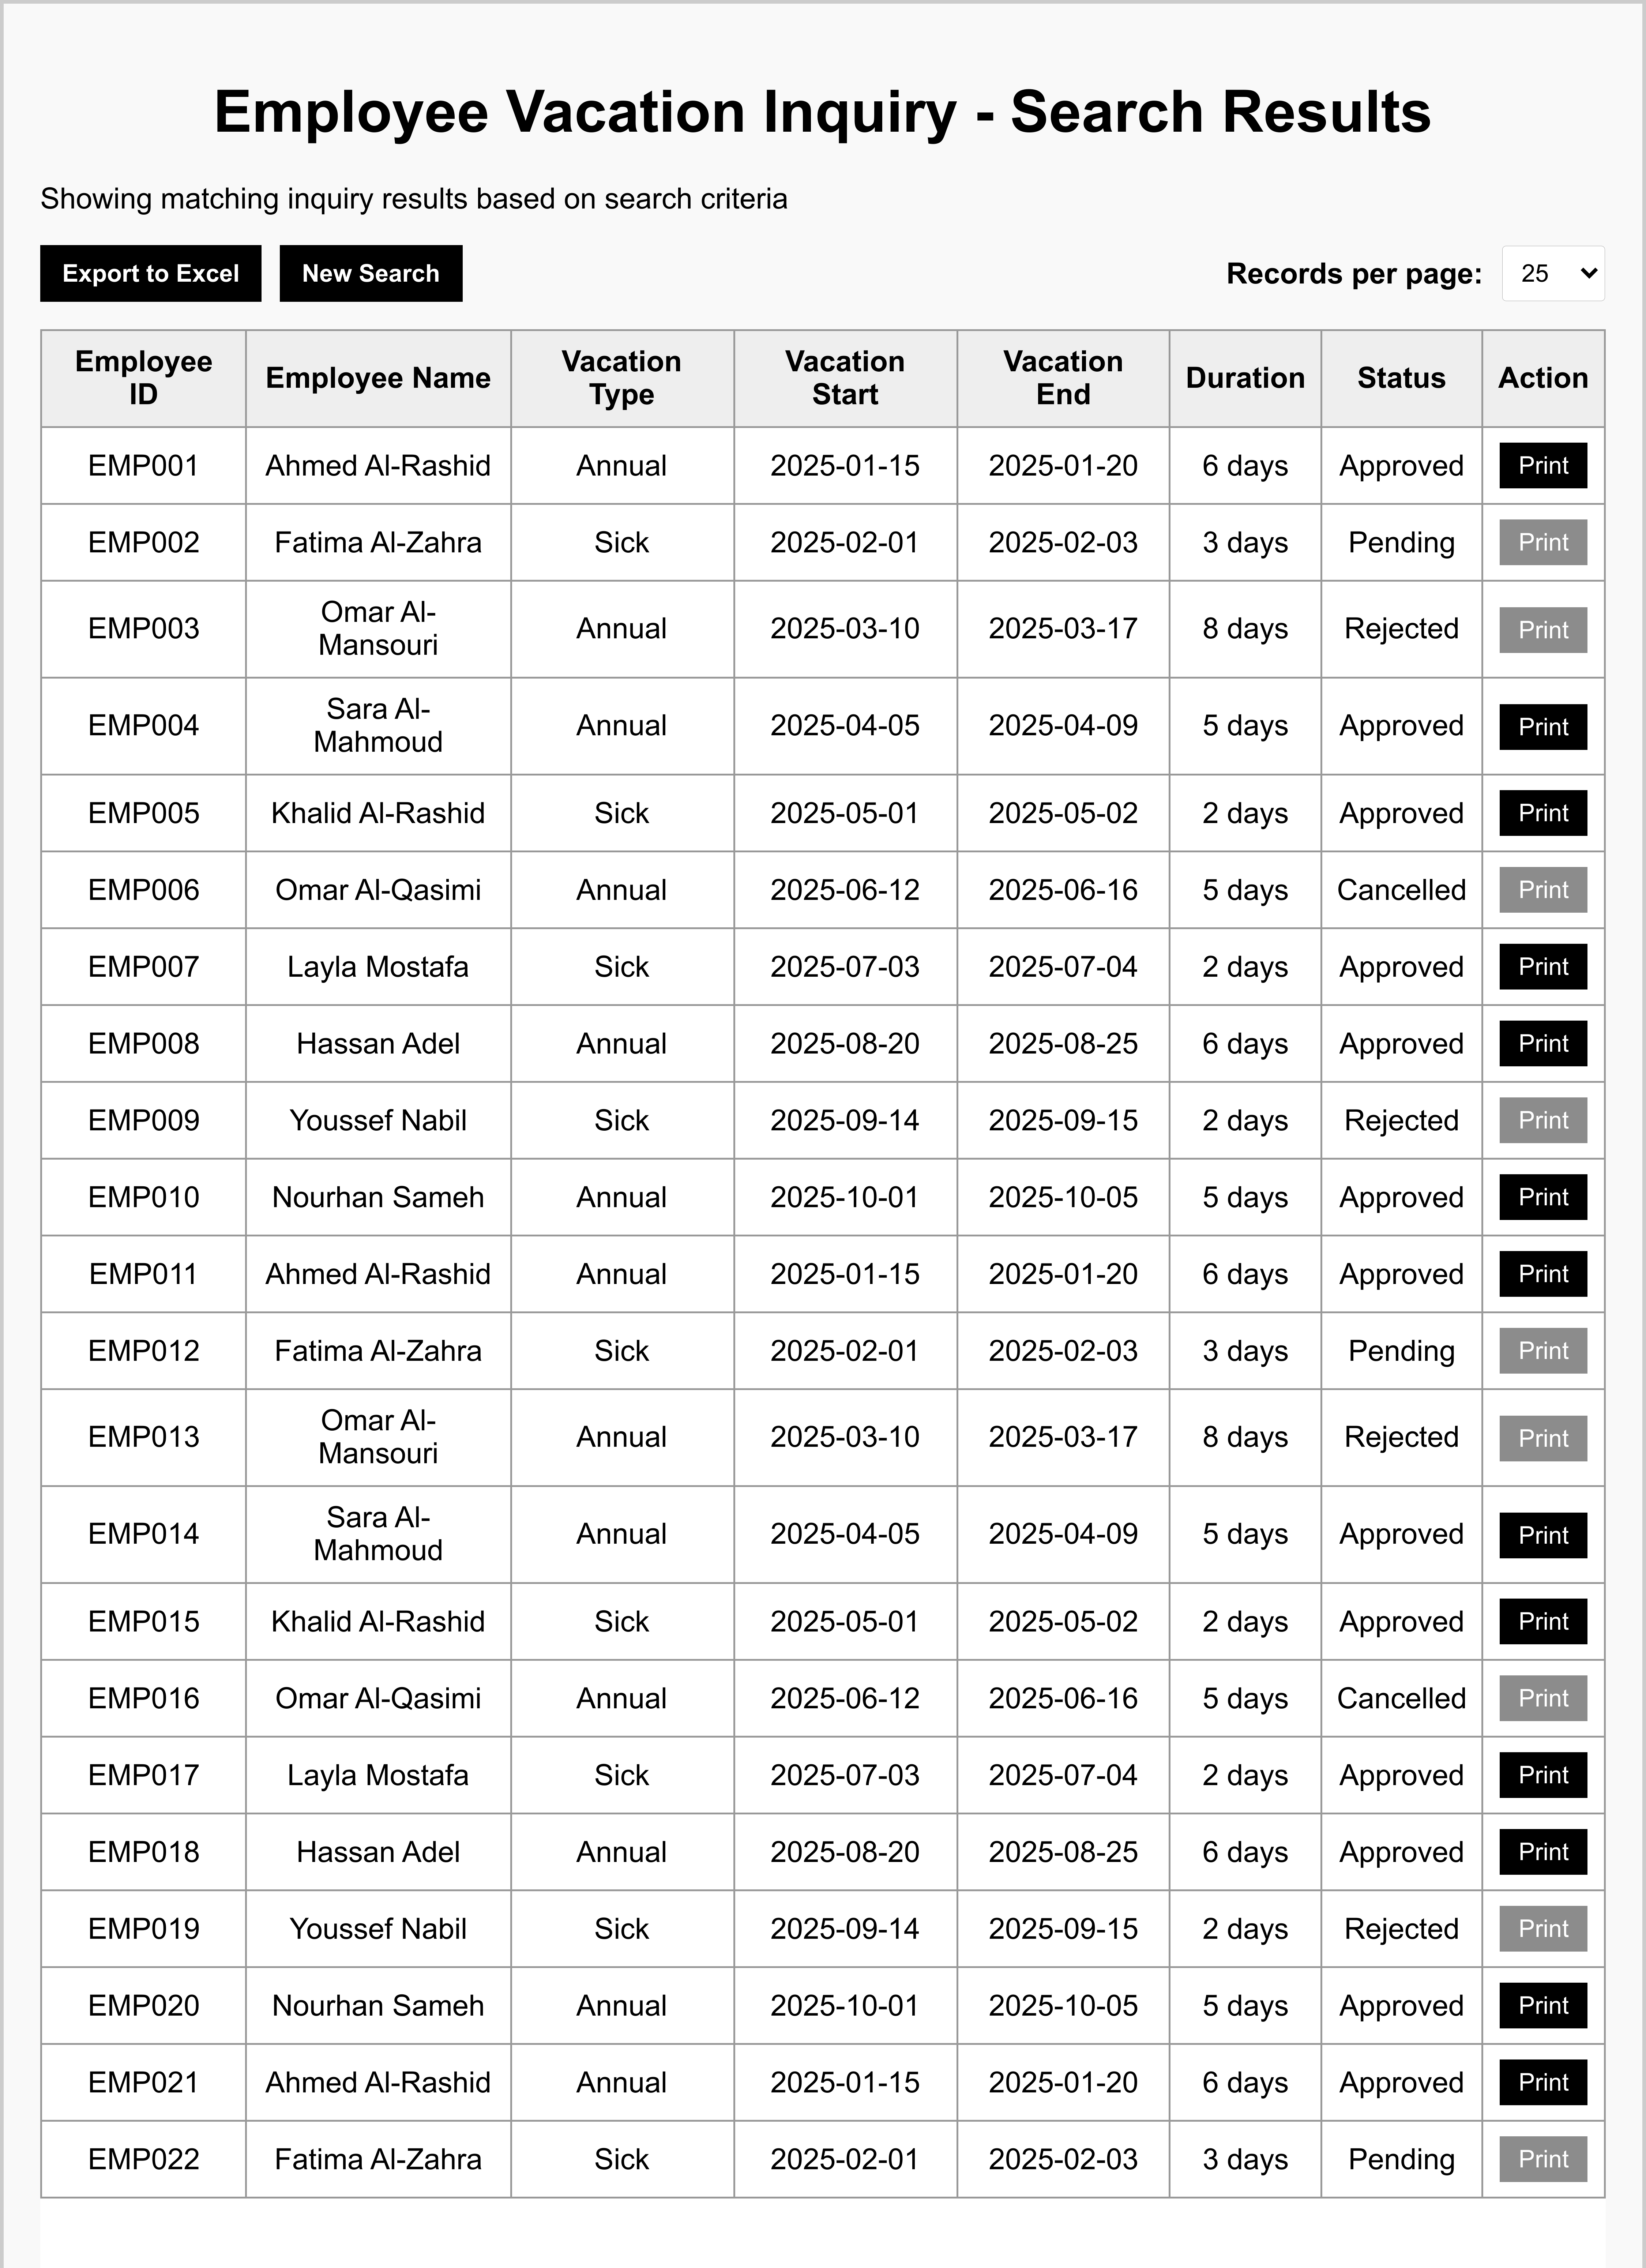
\includegraphics[width=0.9\textwidth]{Wireframes/Employee-Vacation-Inquiry-Search-Results/Employee-Vacation-Inquiry-Search-Results-1.png}
\caption{Vacation Inquiry Search Results Screen}
\label{fig:inquiry-search-results-screen}
\end{figure}

\subsubsection{Notifications Center Screen}
\begin{figure}[H]
\centering
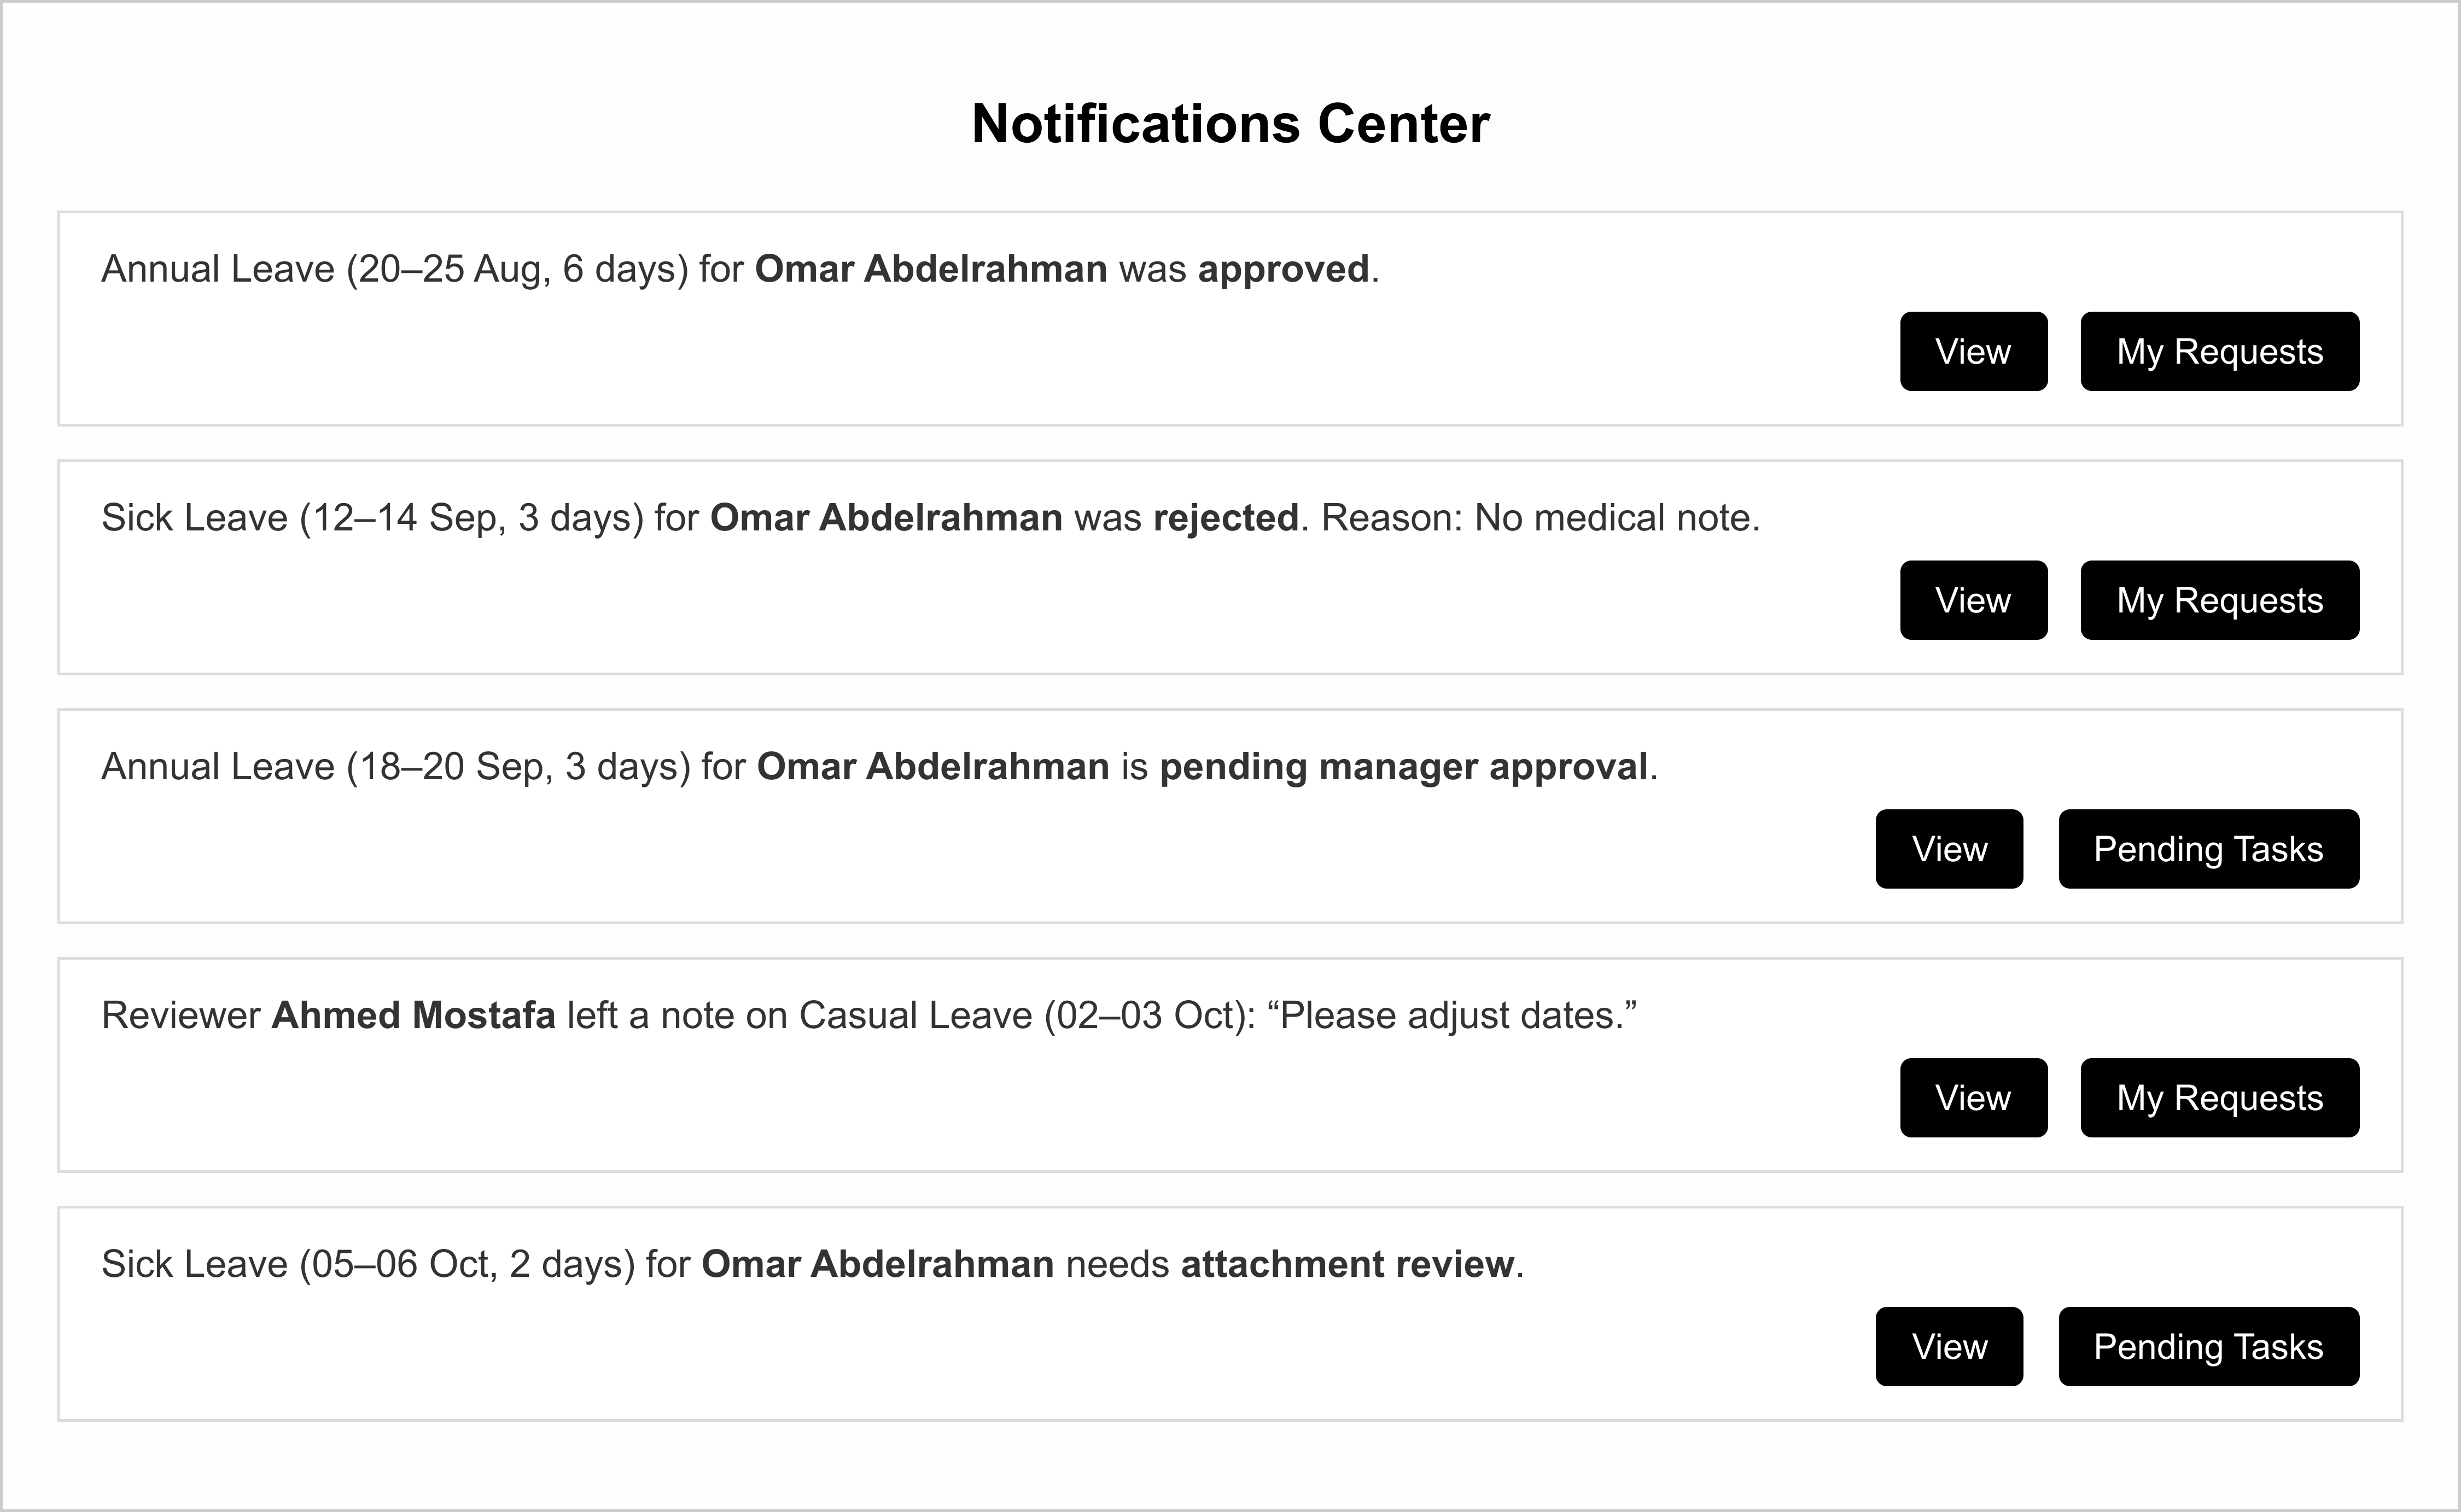
\includegraphics[width=0.9\textwidth]{Wireframes/Notifications-Center/Notifications-Center-1.png}
\caption{Notifications Center Screen}
\label{fig:notifications-center-screen}
\end{figure}

\subsection{Report Layout Screens}

\subsubsection{Single Transaction Report Layout}
\begin{figure}[H]
\centering
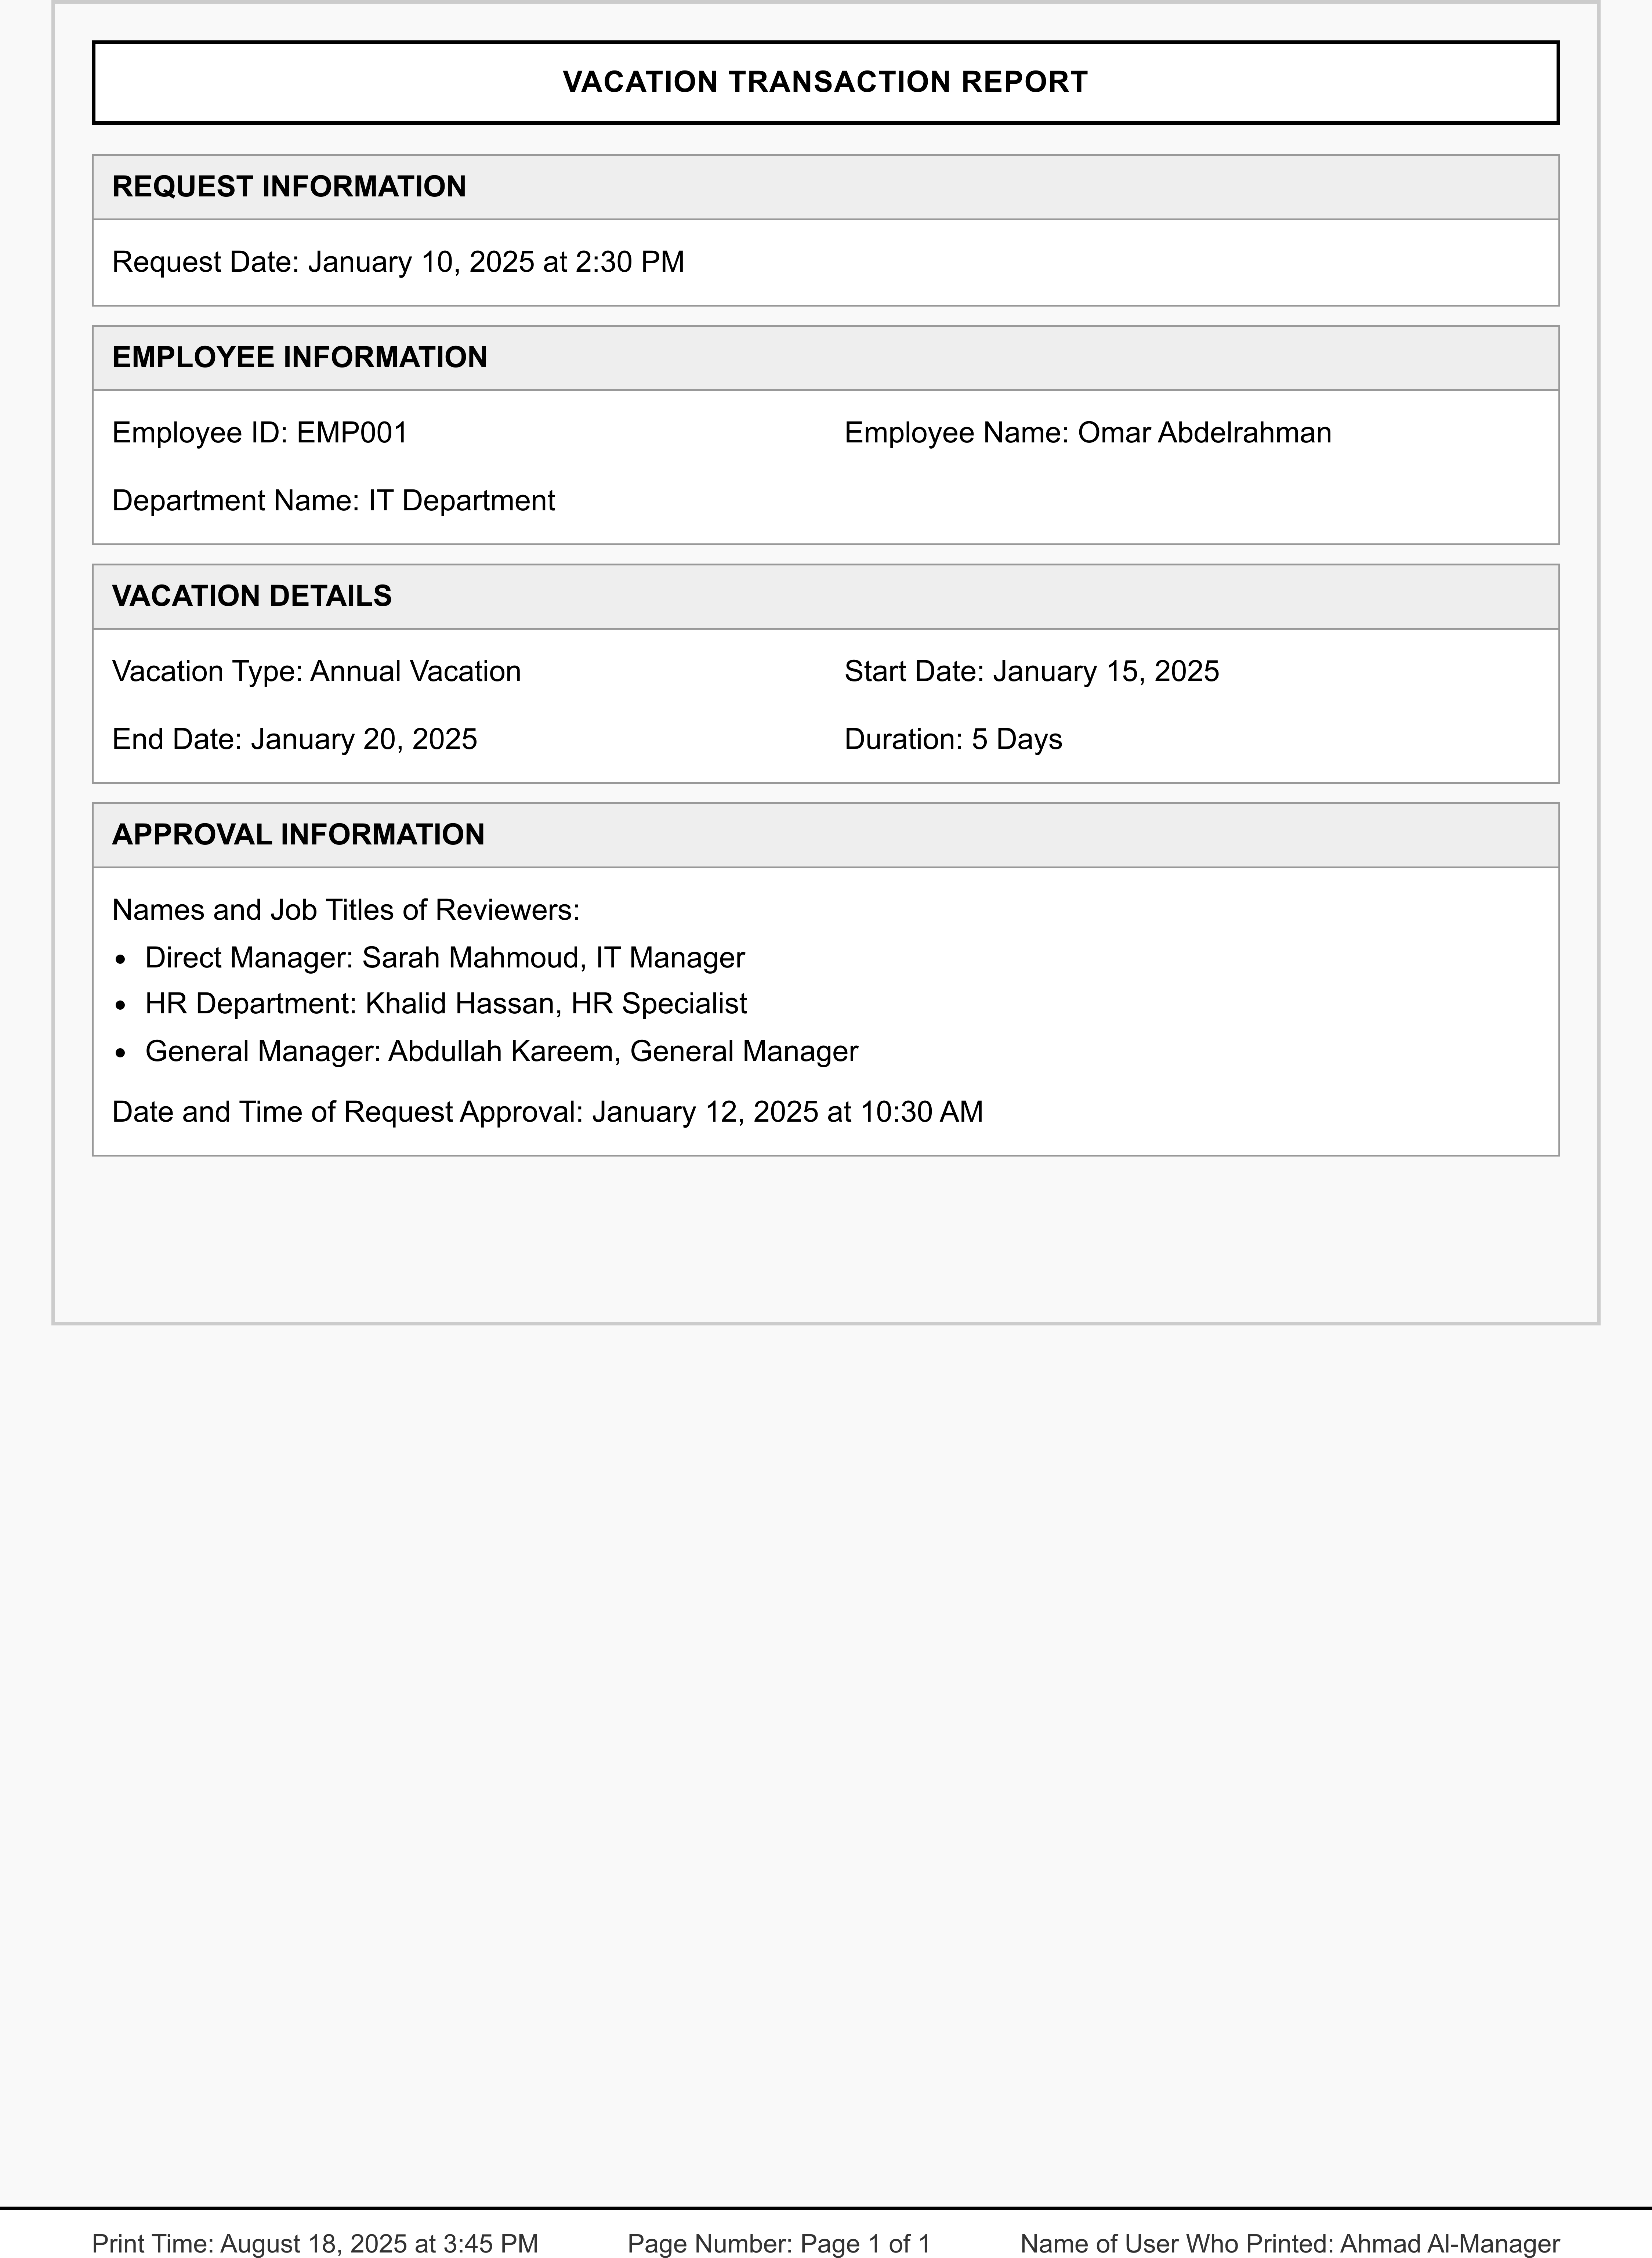
\includegraphics[width=0.9\textwidth]{Wireframes/Print-Layout-Single-Transaction-Report/Print-Layout-Single-Transaction-Report-1.png}
\caption{Single Transaction Report Layout}
\label{fig:single-transaction-report-layout}
\end{figure}

\subsubsection{Annual Comparative Report Layout}
\begin{figure}[H]
\centering
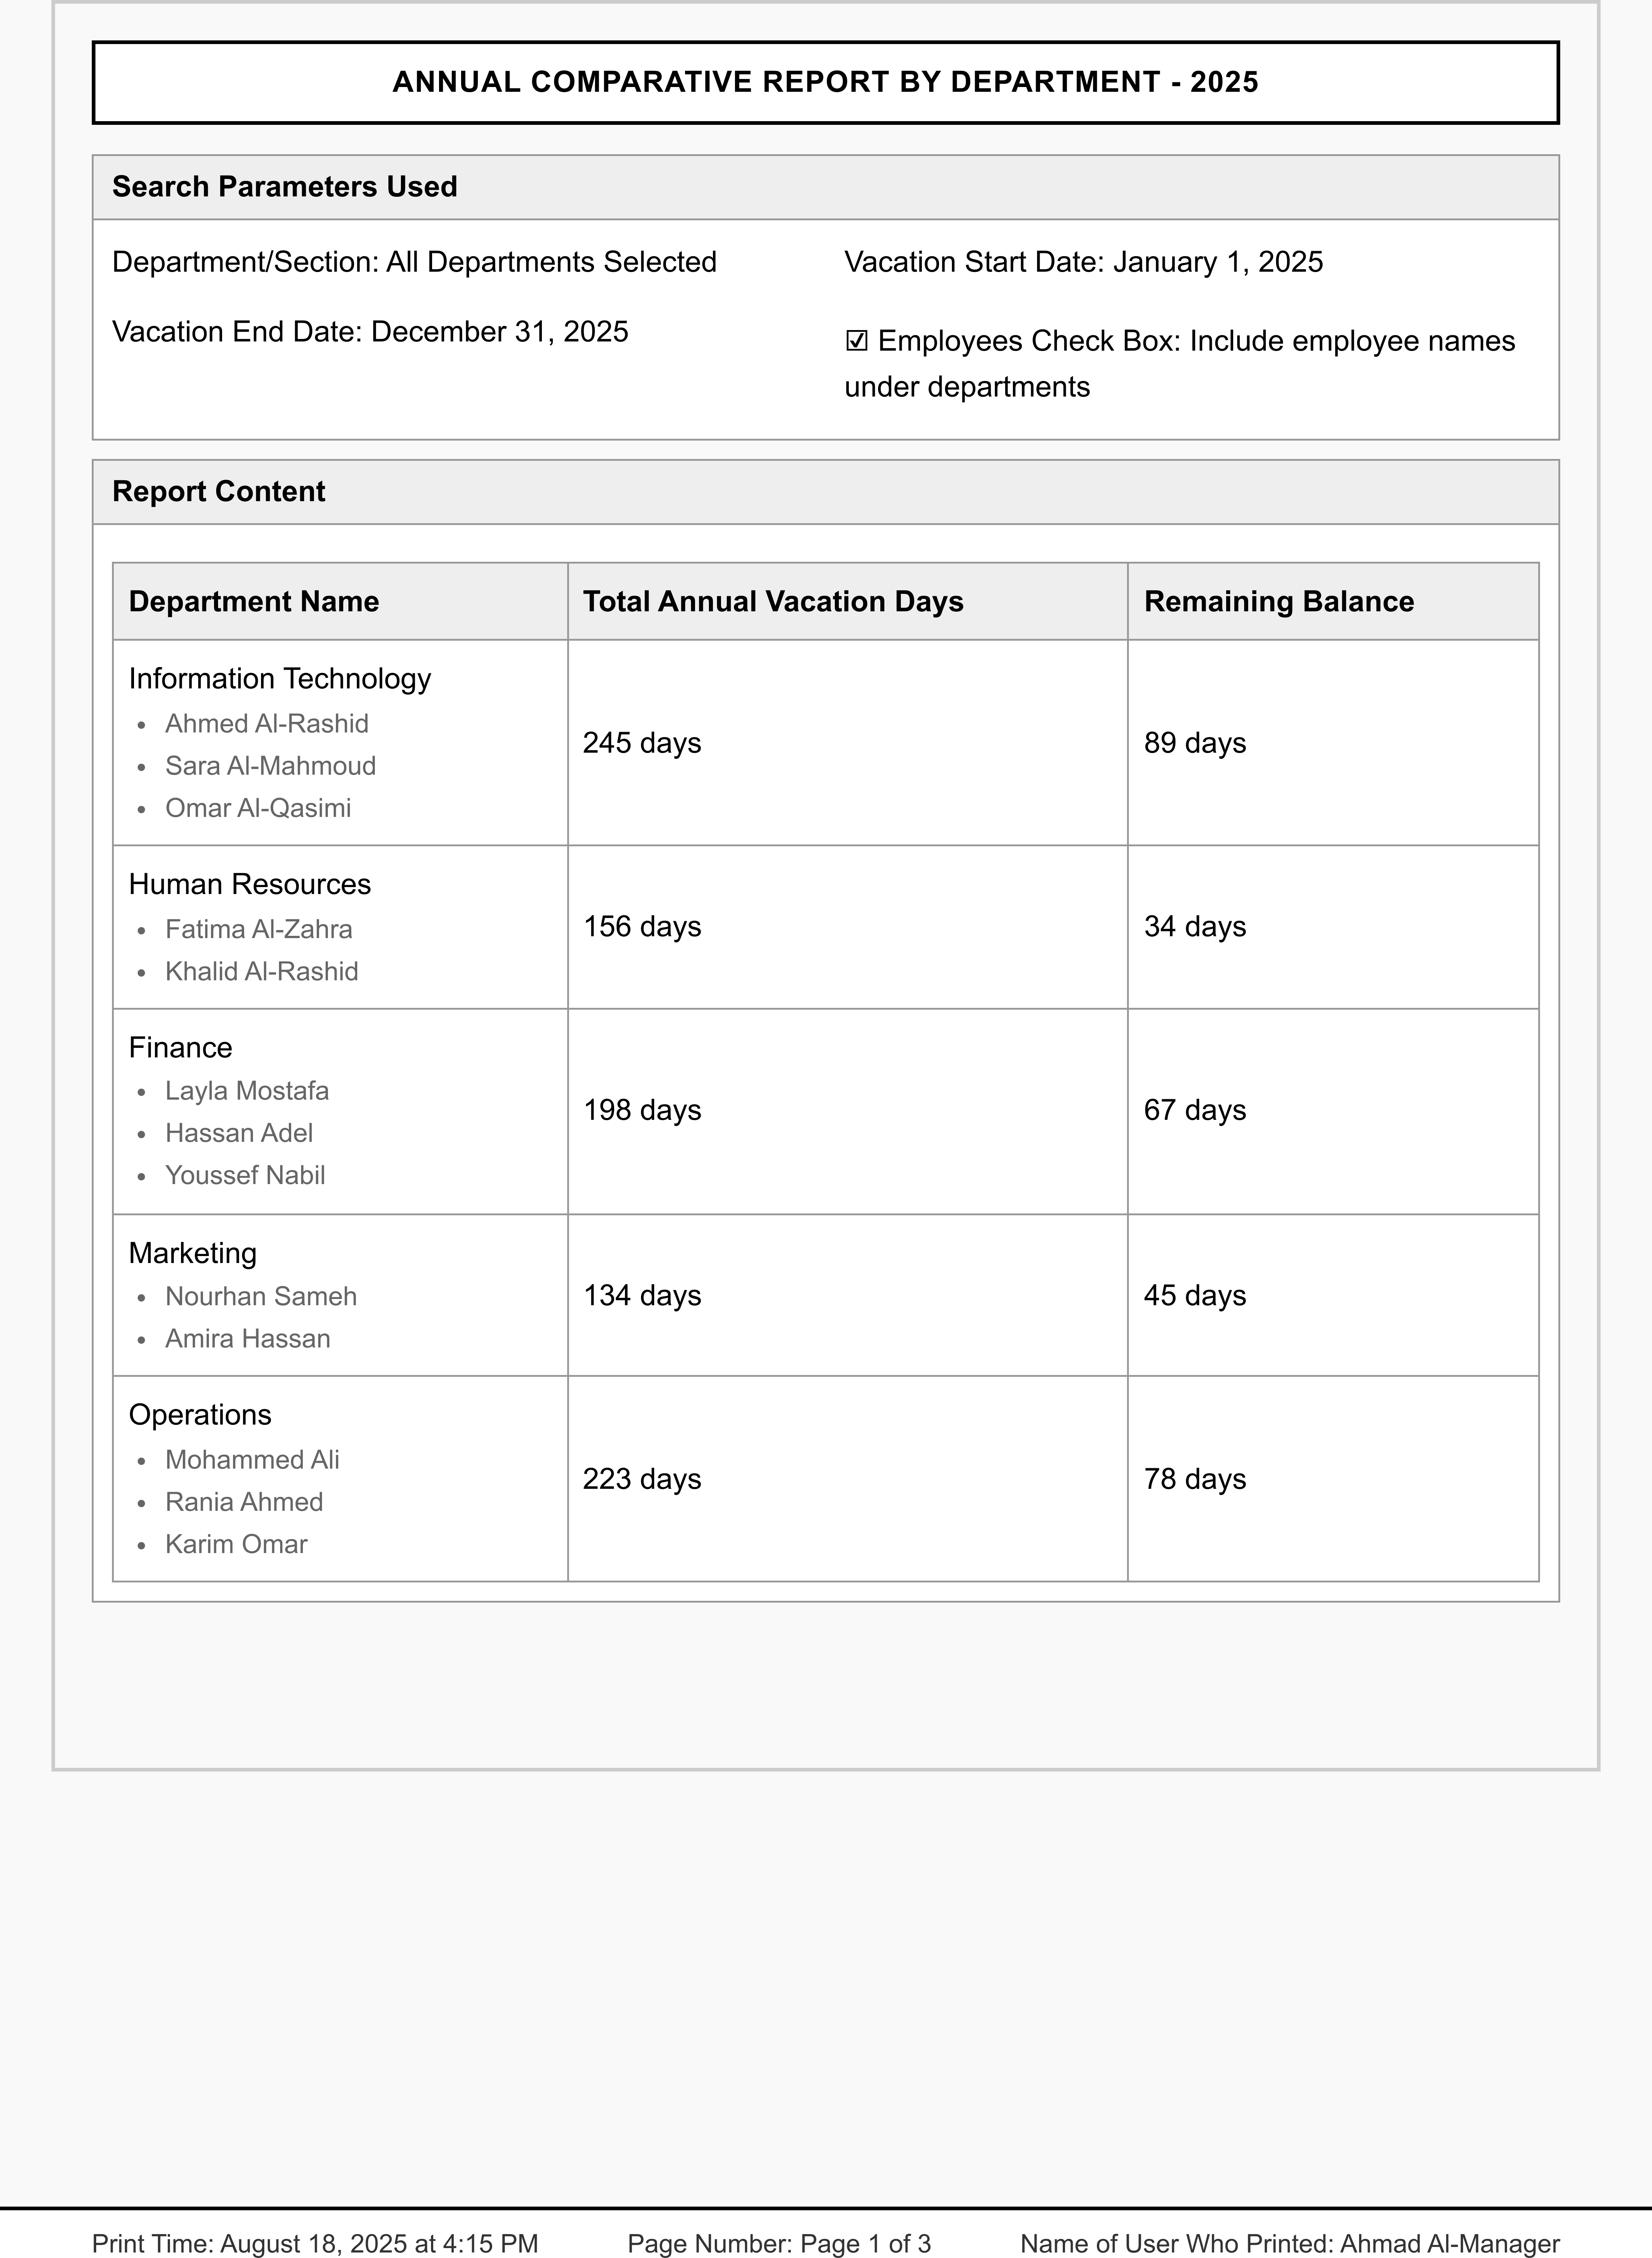
\includegraphics[width=0.9\textwidth]{Wireframes/Print-Layout-Annual-Comparative-Report/Print-Layout-Annual-Comparative-Report-Web-1.png}
\caption{Annual Comparative Report Layout}
\label{fig:annual-comparative-report-layout}
\end{figure}

\subsection{Additional Screens}

\subsubsection{Requests Center}
\begin{figure}[H]
\centering
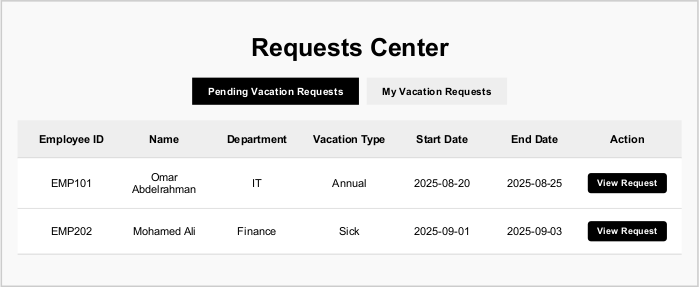
\includegraphics[width=0.9\textwidth]{Wireframes/Requests-Center/Requests-Center-1.png}
\caption{Requests Center Screen}
\label{fig:requests-center-screen}
\end{figure}

\subsubsection{Annual Comparative Report Search Parameters}
\begin{figure}[H]
\centering
\includegraphics[width=0.9\textwidth]{Wireframes/Annual-Comparative-Report-Search-Parameters/Annual-Comparative-Report-Search-Parameters-1.png}
\caption{Annual Comparative Report Search Parameters Screen}
\label{fig:annual-comparative-report-search-params}
\end{figure}

\section{Data Requirements Overview}

This section provides the system's data dictionary specifications and field definitions.

\subsection{Master Data Dictionaries}

\subsubsection{Employee Master Data Dictionary}
\begin{figure}[H]
\centering
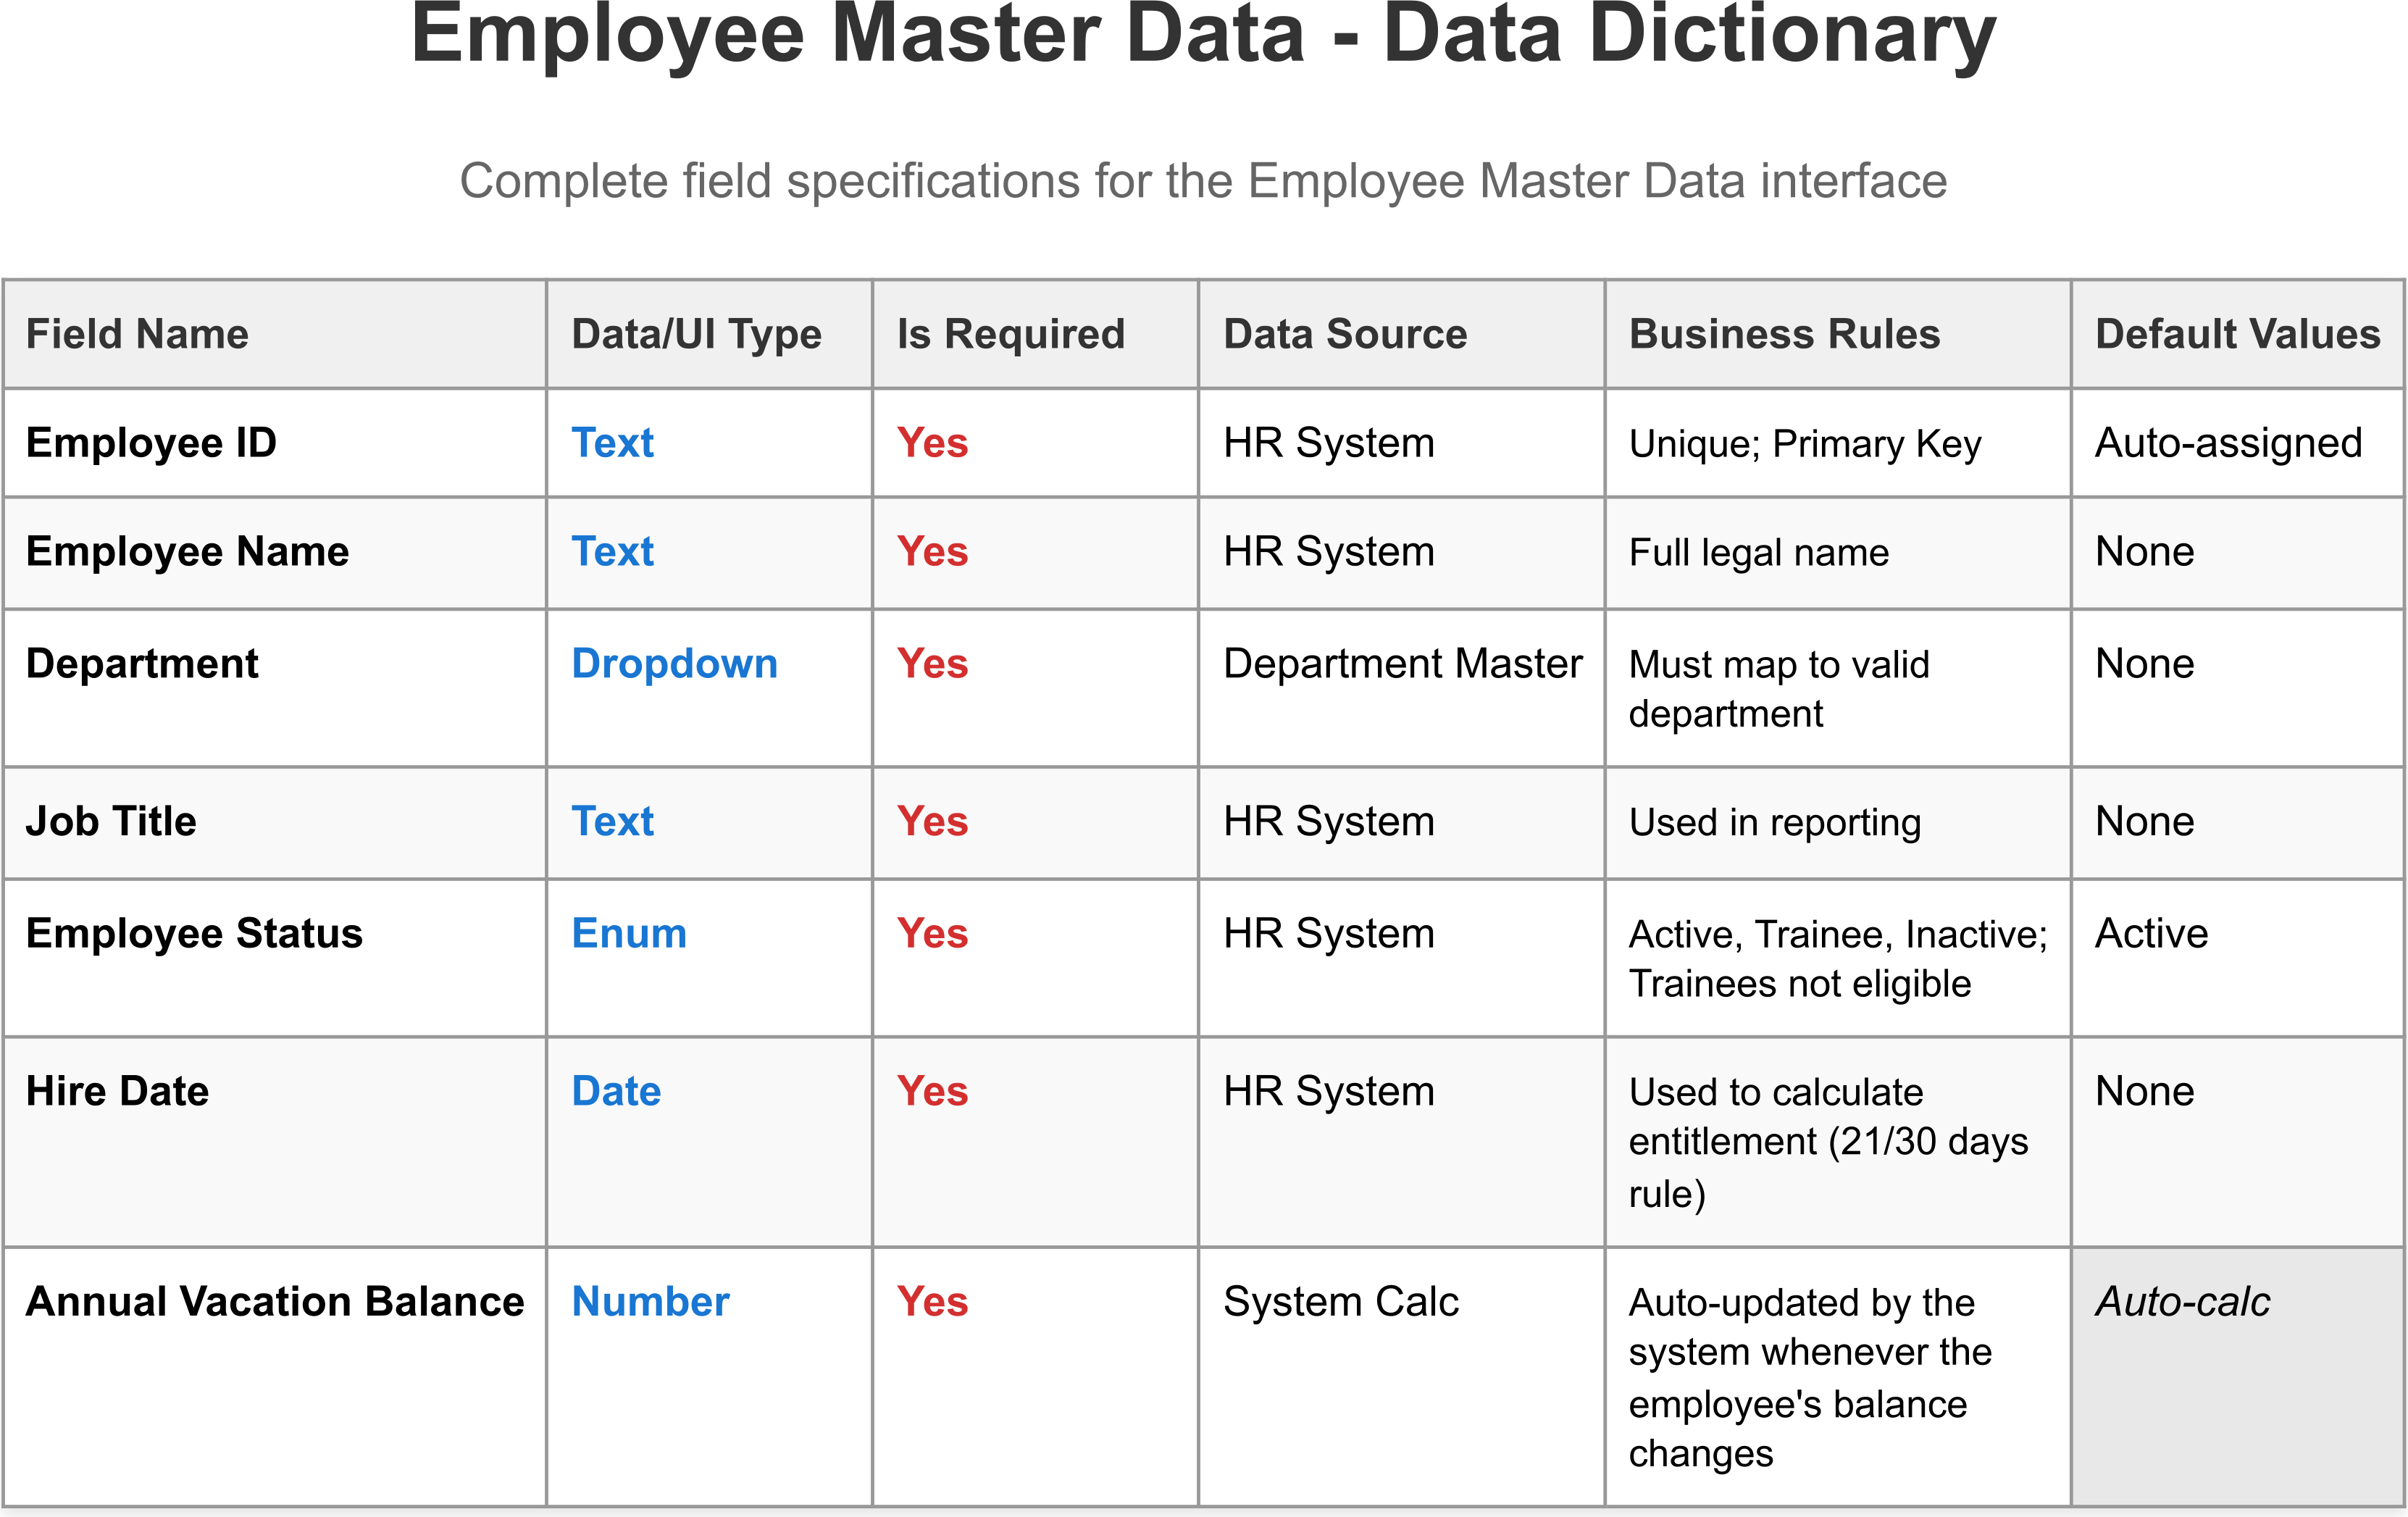
\includegraphics[width=0.9\textwidth]{Data-Dictionary/Master-Data-Dictionaries/Employee-Master-Data-Data-Dictionary/Employee-Master-Data-Data-Dictionary-1.png}
\caption{Employee Master Data Dictionary}
\label{fig:employee-master-data}
\end{figure}

\subsubsection{Departments Master Data Dictionary}
\begin{figure}[H]
\centering
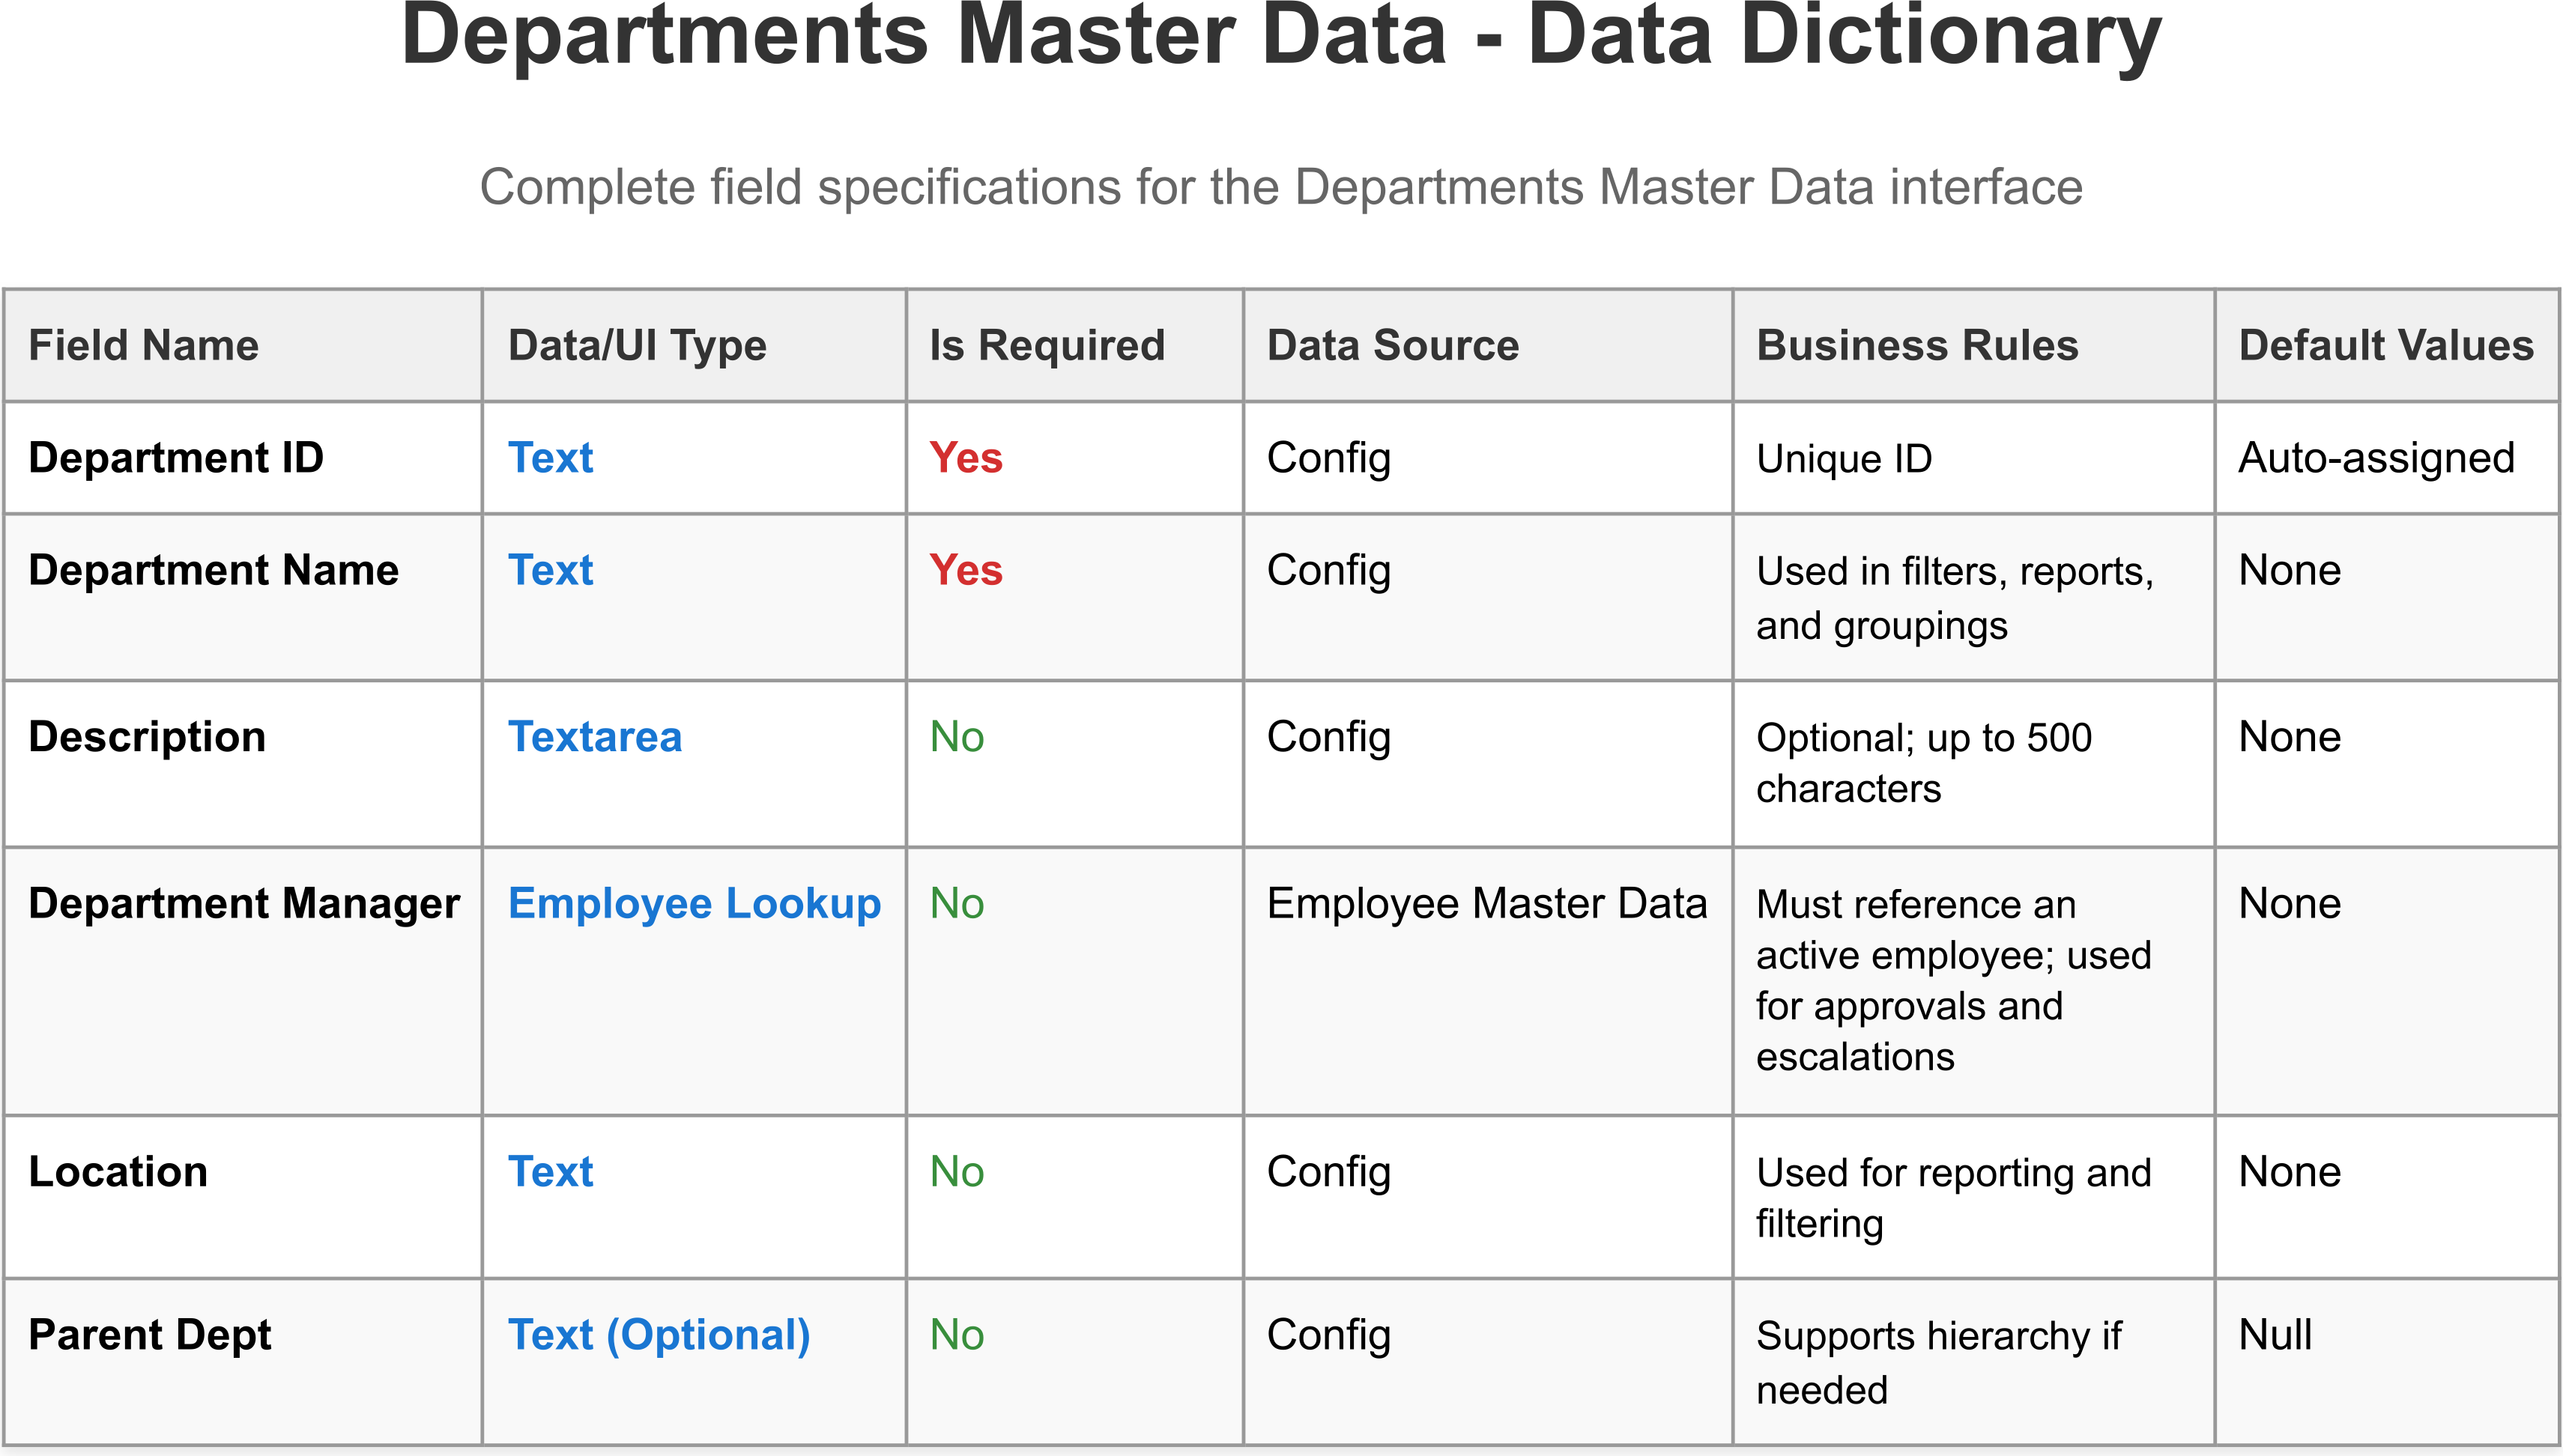
\includegraphics[width=0.9\textwidth]{Data-Dictionary/Master-Data-Dictionaries/Departments-Master-Data-Data-Dictionary/Departments-Master-Data-Data-Dictionary-1.png}
\caption{Departments Master Data Dictionary}
\label{fig:departments-master-data}
\end{figure}

\subsubsection{Vacation Types Master Data Dictionary}
\begin{figure}[H]
\centering
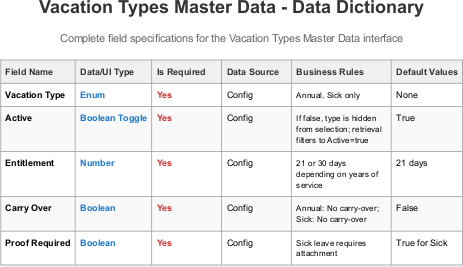
\includegraphics[width=0.9\textwidth]{Data-Dictionary/Master-Data-Dictionaries/Vacation-Types-Master-Data-Data-Dictionary/Vacation-Types-Master-Data-Data-Dictionary-1.png}
\caption{Vacation Types Master Data Dictionary}
\label{fig:vacation-types-master-data}
\end{figure}

\subsection{Screen-Level Data Dictionaries}

\subsubsection{Vacation Request Screen Data Dictionary}
\begin{figure}[H]
\centering
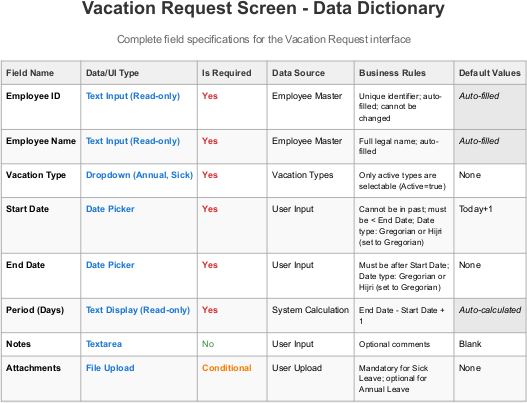
\includegraphics[width=0.9\textwidth]{Data-Dictionary/Screen-Data-Dictionaries/Vacation-Request-Screen-Data-Dictionary/Vacation-Request-Screen-Data-Dictionary-1.png}
\caption{Vacation Request Screen Data Dictionary}
\label{fig:vacation-request-data-dict}
\end{figure}

\subsubsection{Vacation Cancellation Request Screen Data Dictionary}
\begin{figure}[H]
\centering
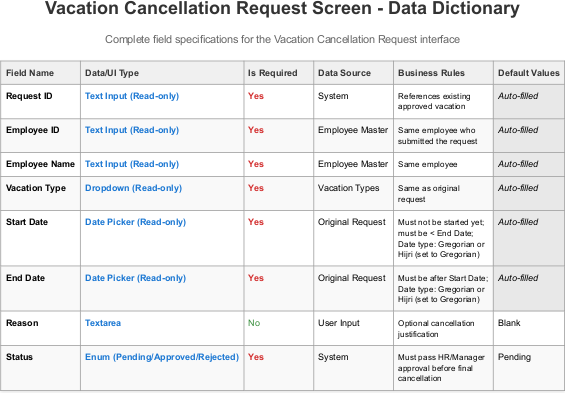
\includegraphics[width=0.9\textwidth]{Data-Dictionary/Screen-Data-Dictionaries/Vacation-Cancellation-Request-Screen-Data-Dictionary/Vacation-Cancellation-Request-Screen-Data-Dictionary-1.png}
\caption{Vacation Cancellation Request Screen Data Dictionary}
\label{fig:vacation-cancellation-data-dict}
\end{figure}

\subsubsection{Review Vacation Request Screen Data Dictionary}
\begin{figure}[H]
\centering
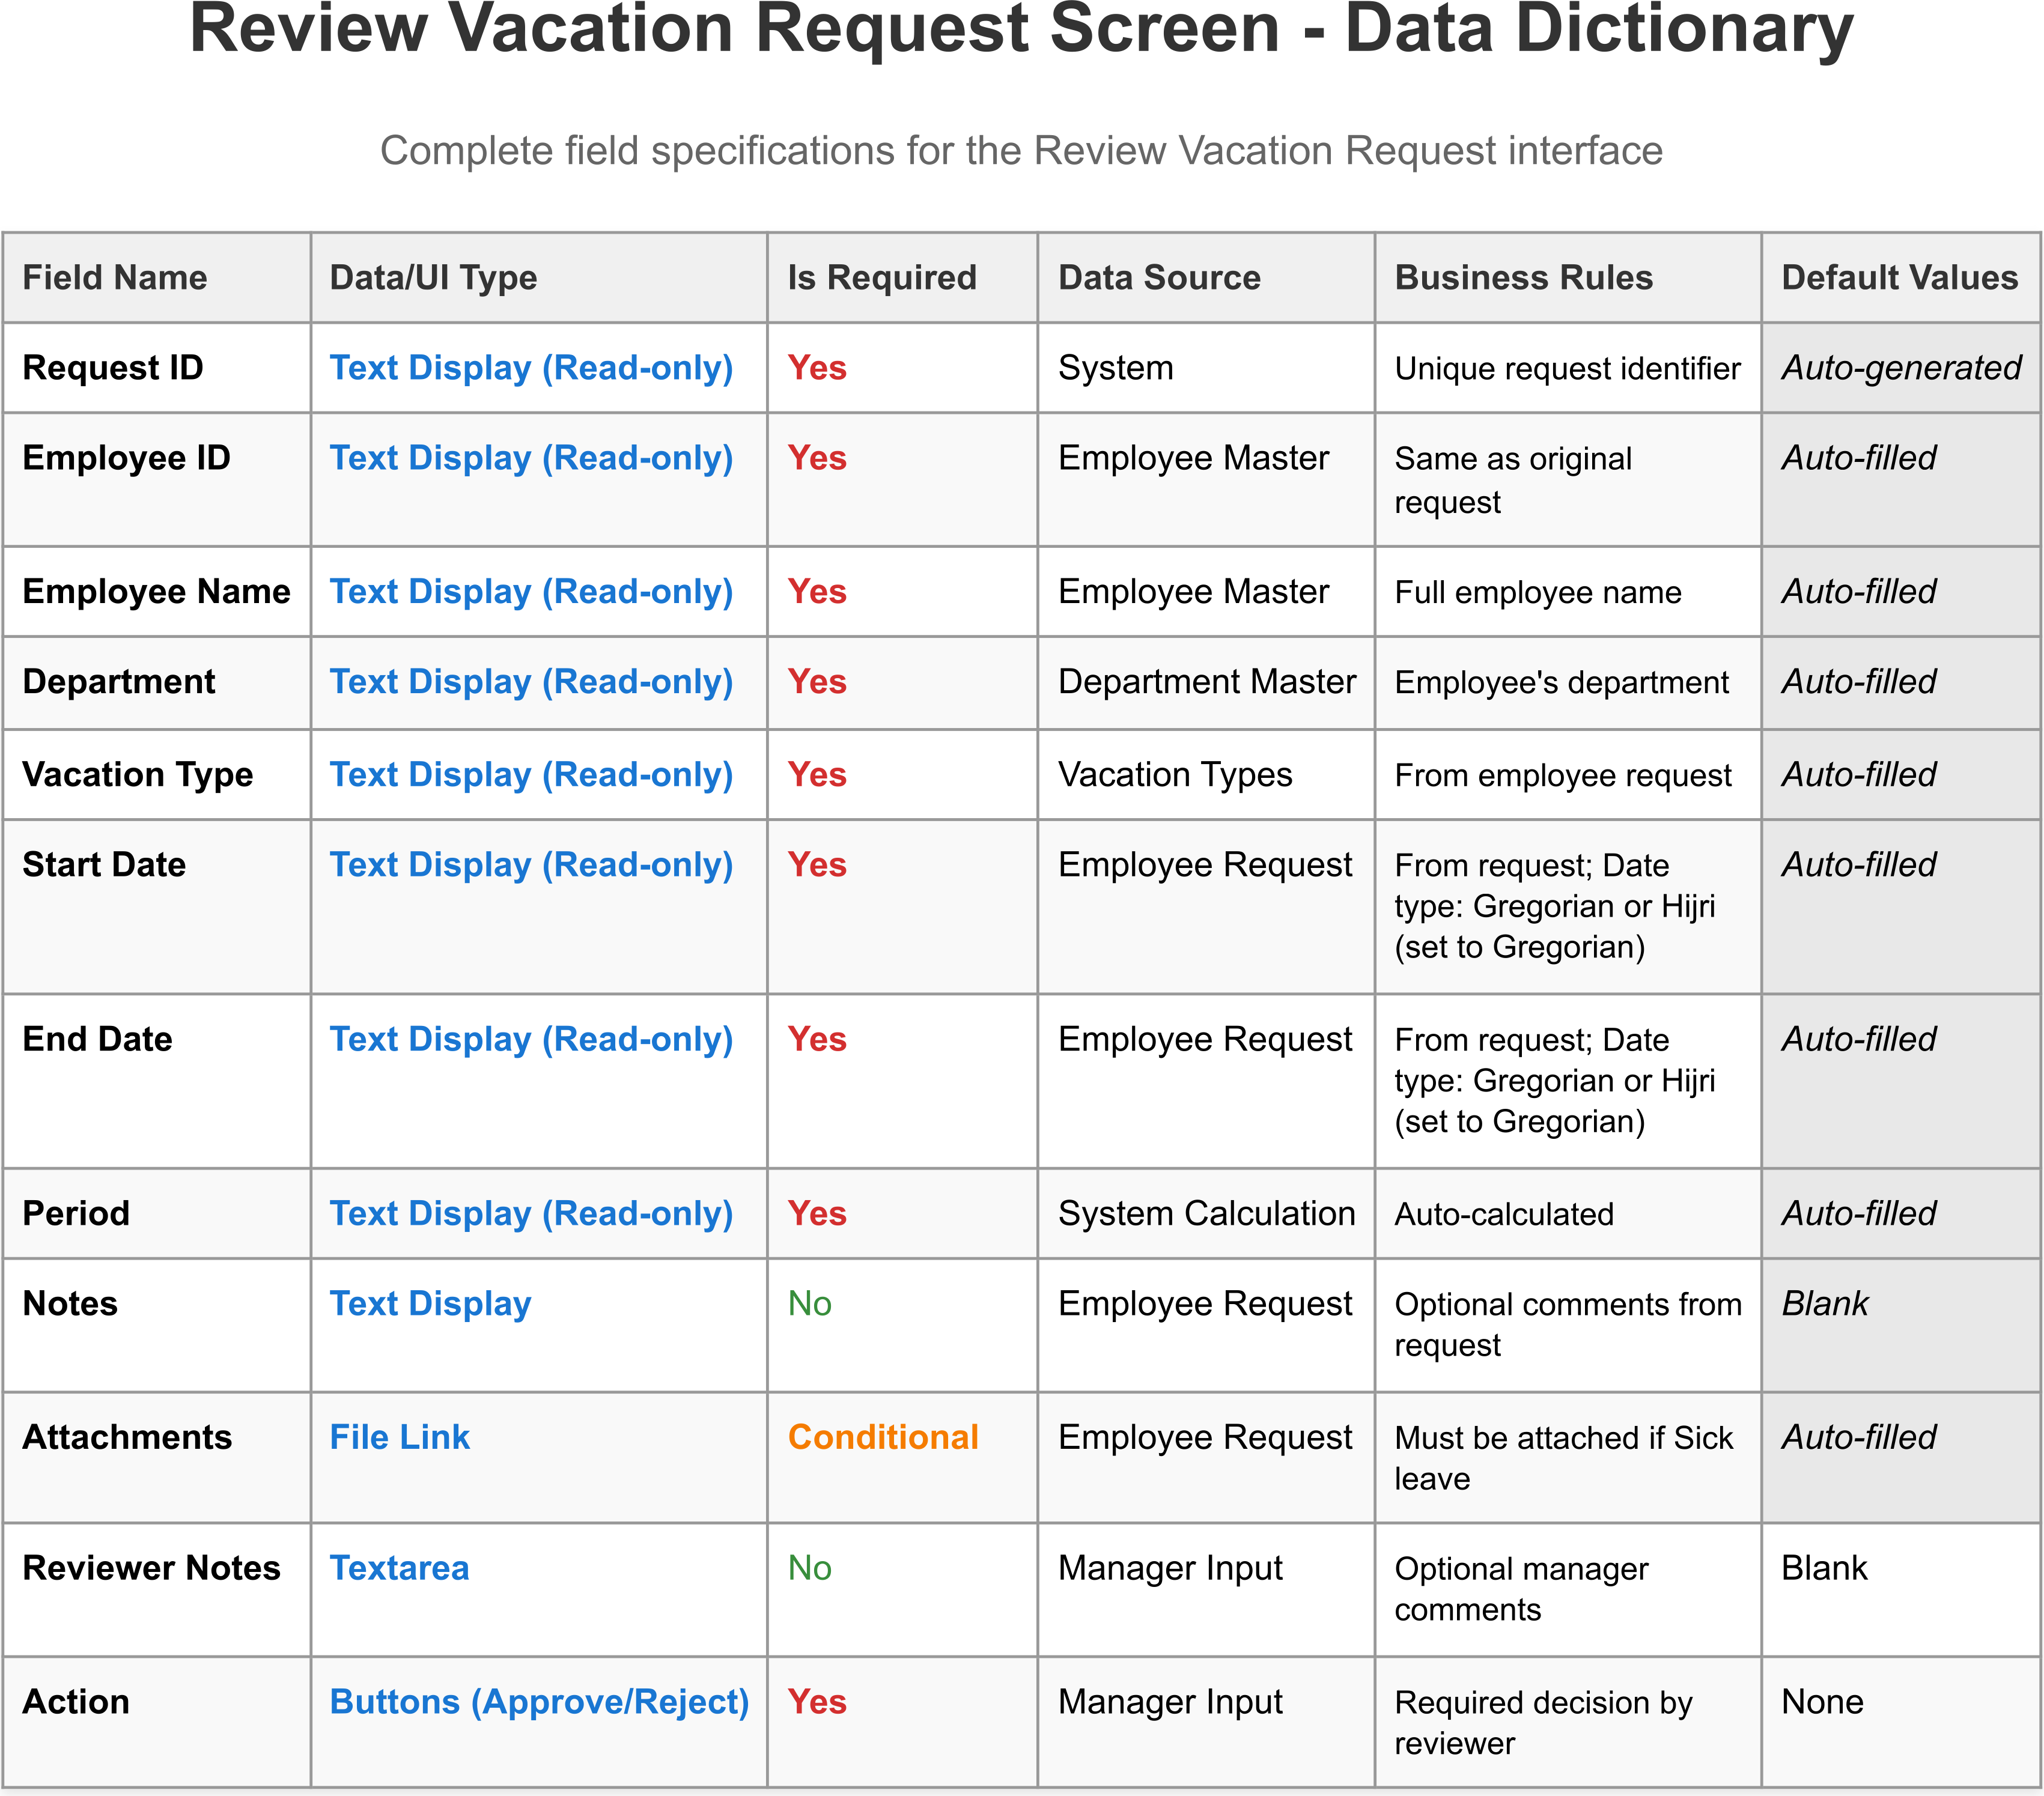
\includegraphics[width=0.9\textwidth]{Data-Dictionary/Screen-Data-Dictionaries/Review-Vacation-Request-Screen-Data-Dictionary/Review-Vacation-Request-Screen-Data-Dictionary-1.png}
\caption{Review Vacation Request Screen Data Dictionary}
\label{fig:review-vacation-data-dict}
\end{figure}

\subsubsection{Review Vacation Cancellation Request Screen Data Dictionary}
\begin{figure}[H]
\centering
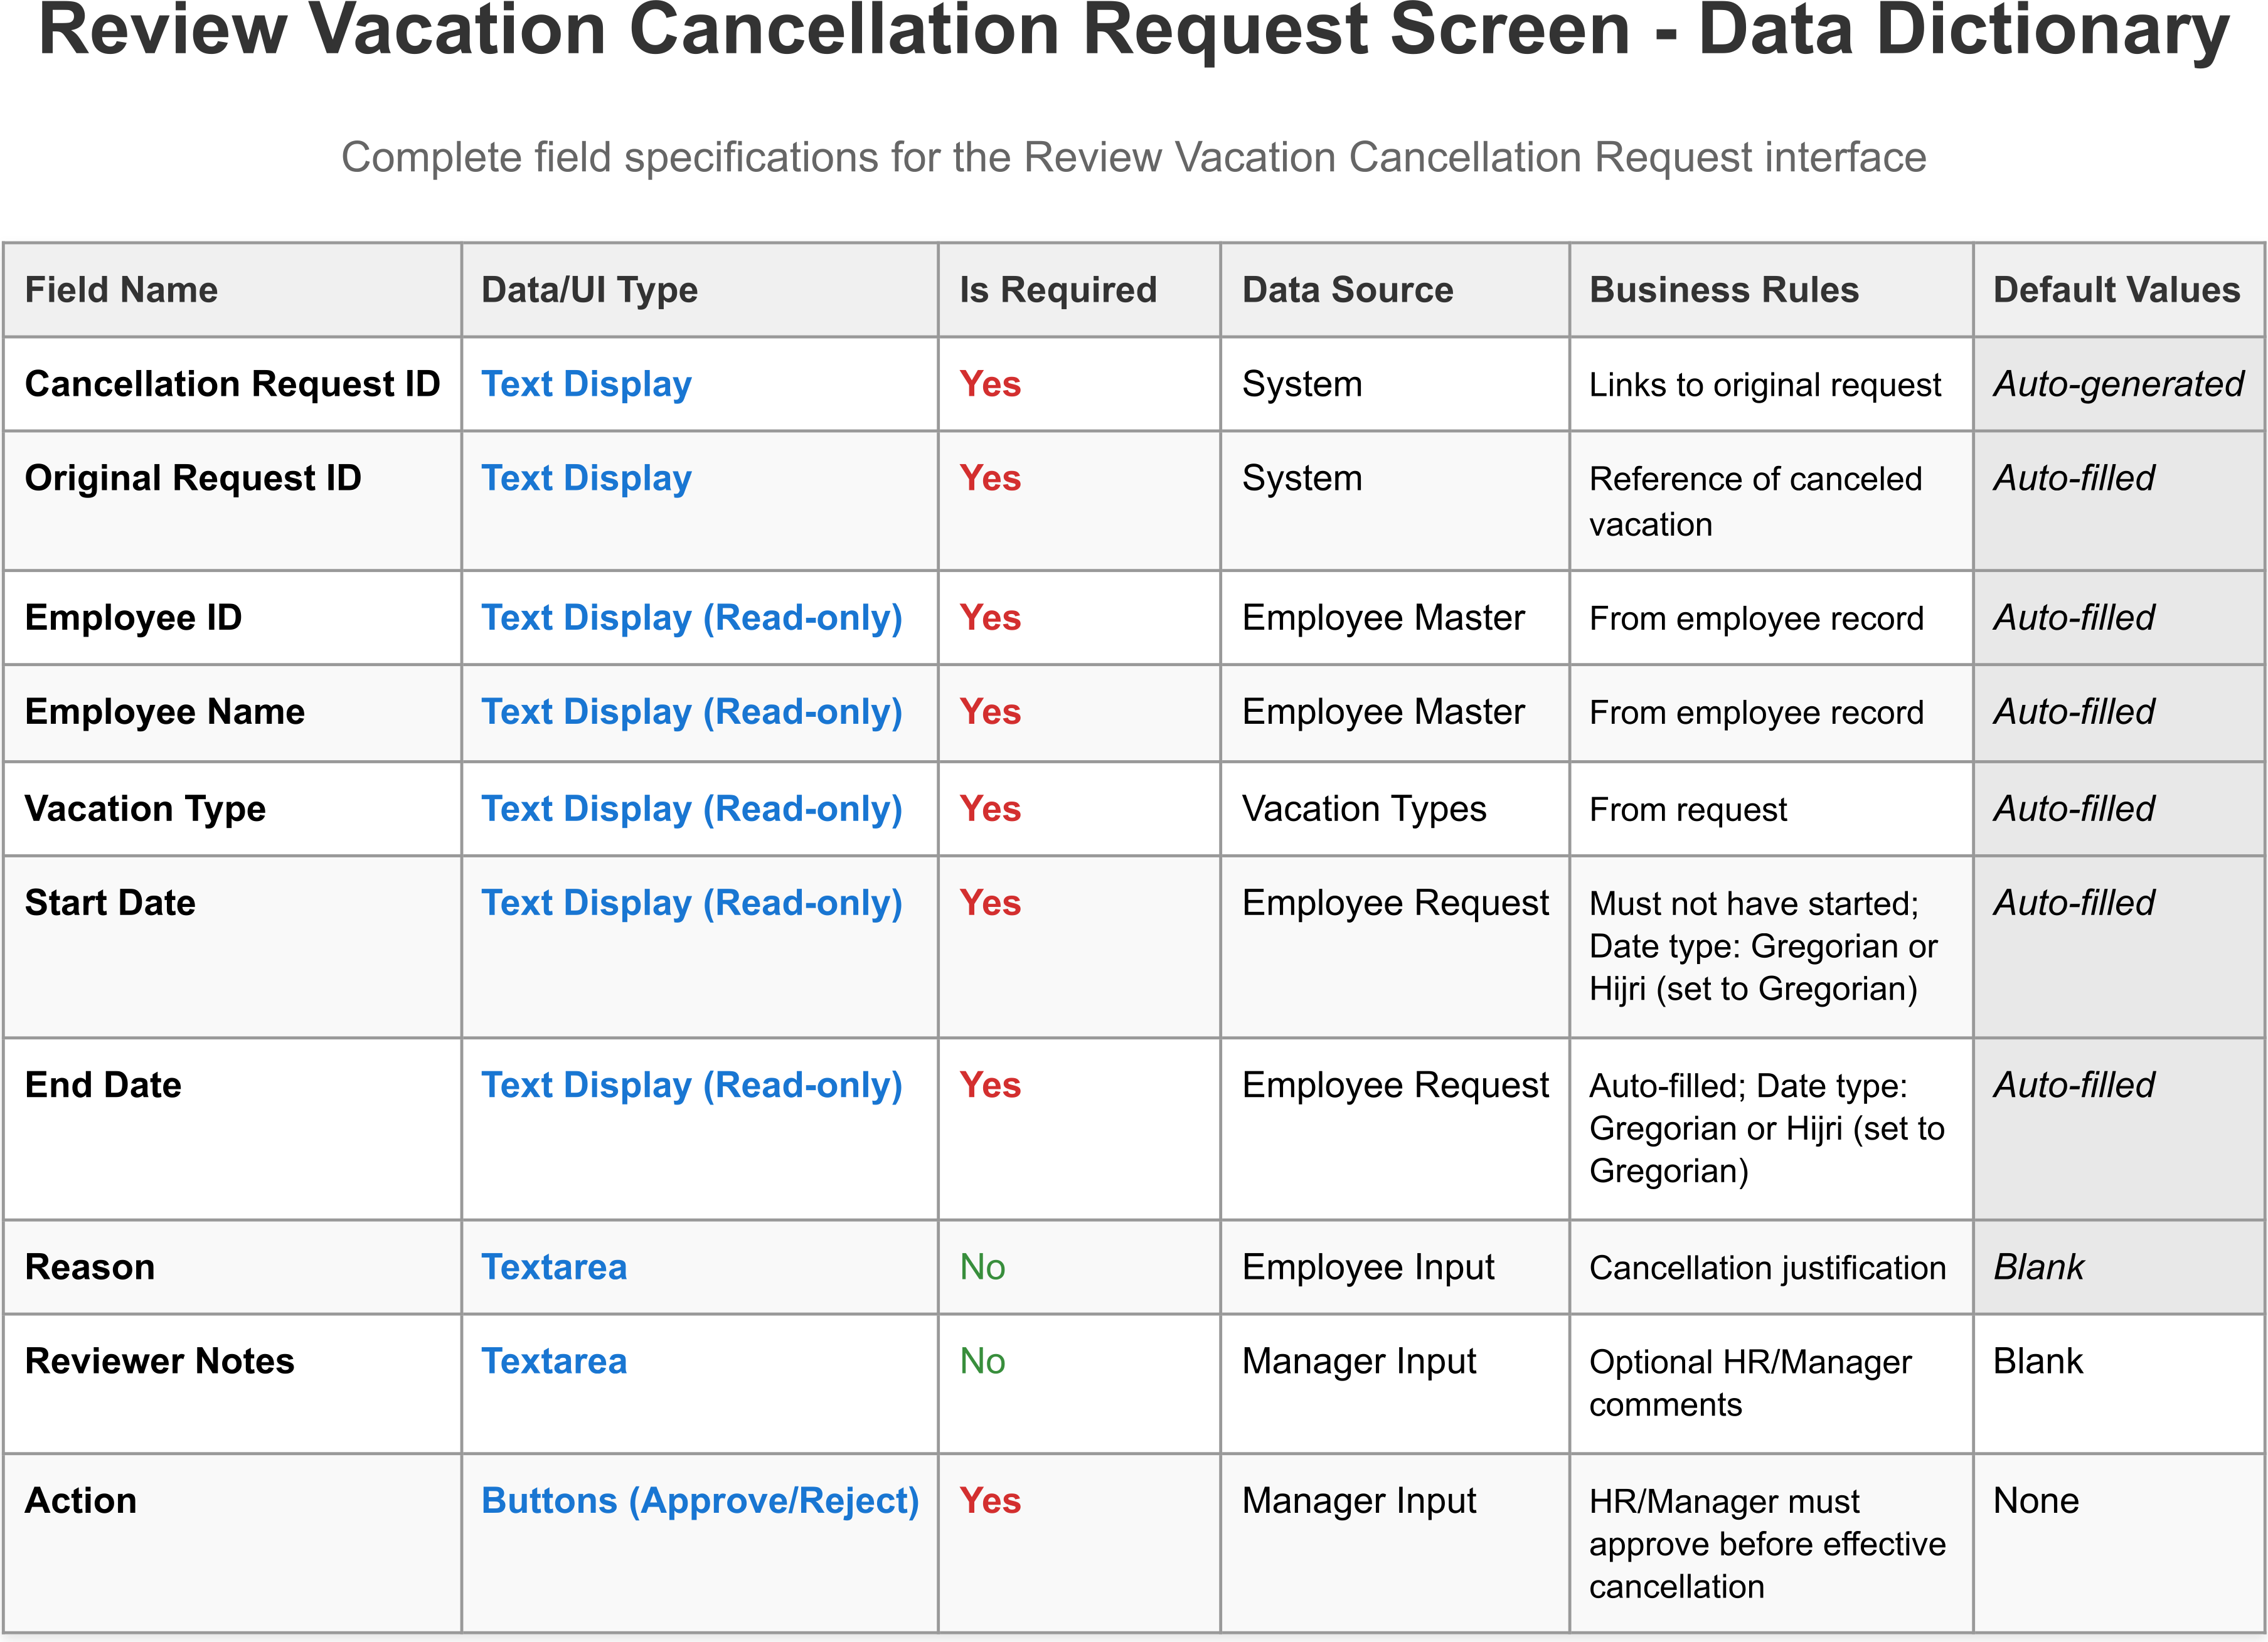
\includegraphics[width=0.9\textwidth]{Data-Dictionary/Screen-Data-Dictionaries/Review-Vacation-Cancellation-Request-Screen-Data-Dictionary/Review-Vacation-Cancellation-Request-Screen-Data-Dictionary-1.png}
\caption{Review Vacation Cancellation Request Screen Data Dictionary}
\label{fig:review-cancellation-data-dict}
\end{figure}

\subsubsection{My Vacation Requests Screen Data Dictionary}
\begin{figure}[H]
\centering
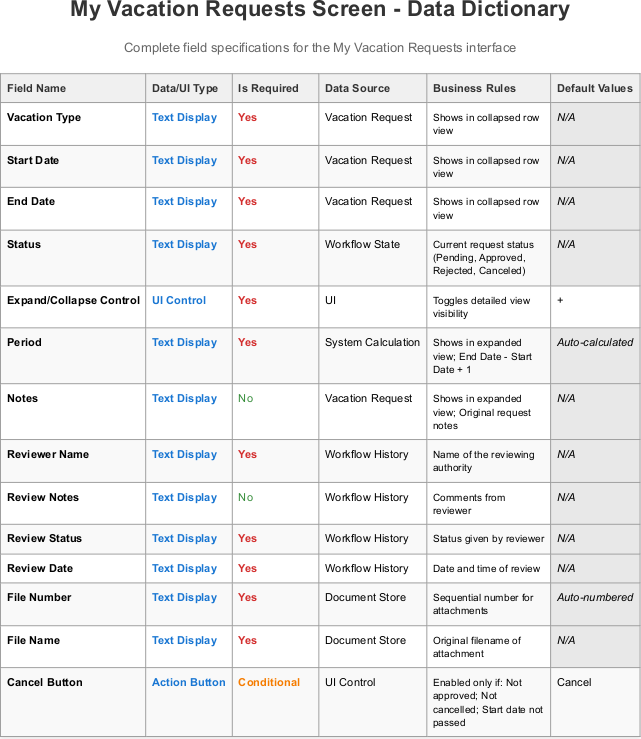
\includegraphics[width=0.9\textwidth]{Data-Dictionary/Screen-Data-Dictionaries/My-Vacation-Requests-Screen-Data-Dictionary/My-Vacation-Requests-Screen-Data-Dictionary-1.png}
\caption{My Vacation Requests Screen Data Dictionary}
\label{fig:my-vacation-requests-data-dict}
\end{figure}

\subsubsection{Pending Vacation Requests Screen Data Dictionary}
\begin{figure}[H]
\centering
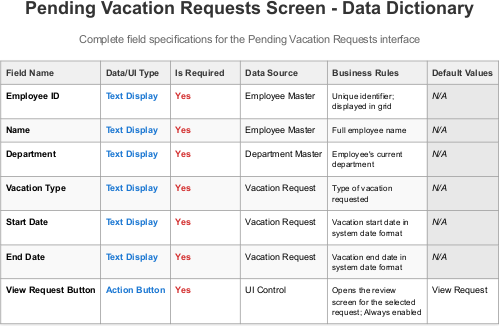
\includegraphics[width=0.9\textwidth]{Data-Dictionary/Screen-Data-Dictionaries/Pending-Vacation-Requests-Screen-Data-Dictionary/Pending-Vacation-Requests-Screen-Data-Dictionary-1.png}
\caption{Pending Vacation Requests Screen Data Dictionary}
\label{fig:pending-vacation-requests-data-dict}
\end{figure}

\subsubsection{Vacation Inquiry Search Parameters Screen Data Dictionary}
\begin{figure}[H]
\centering
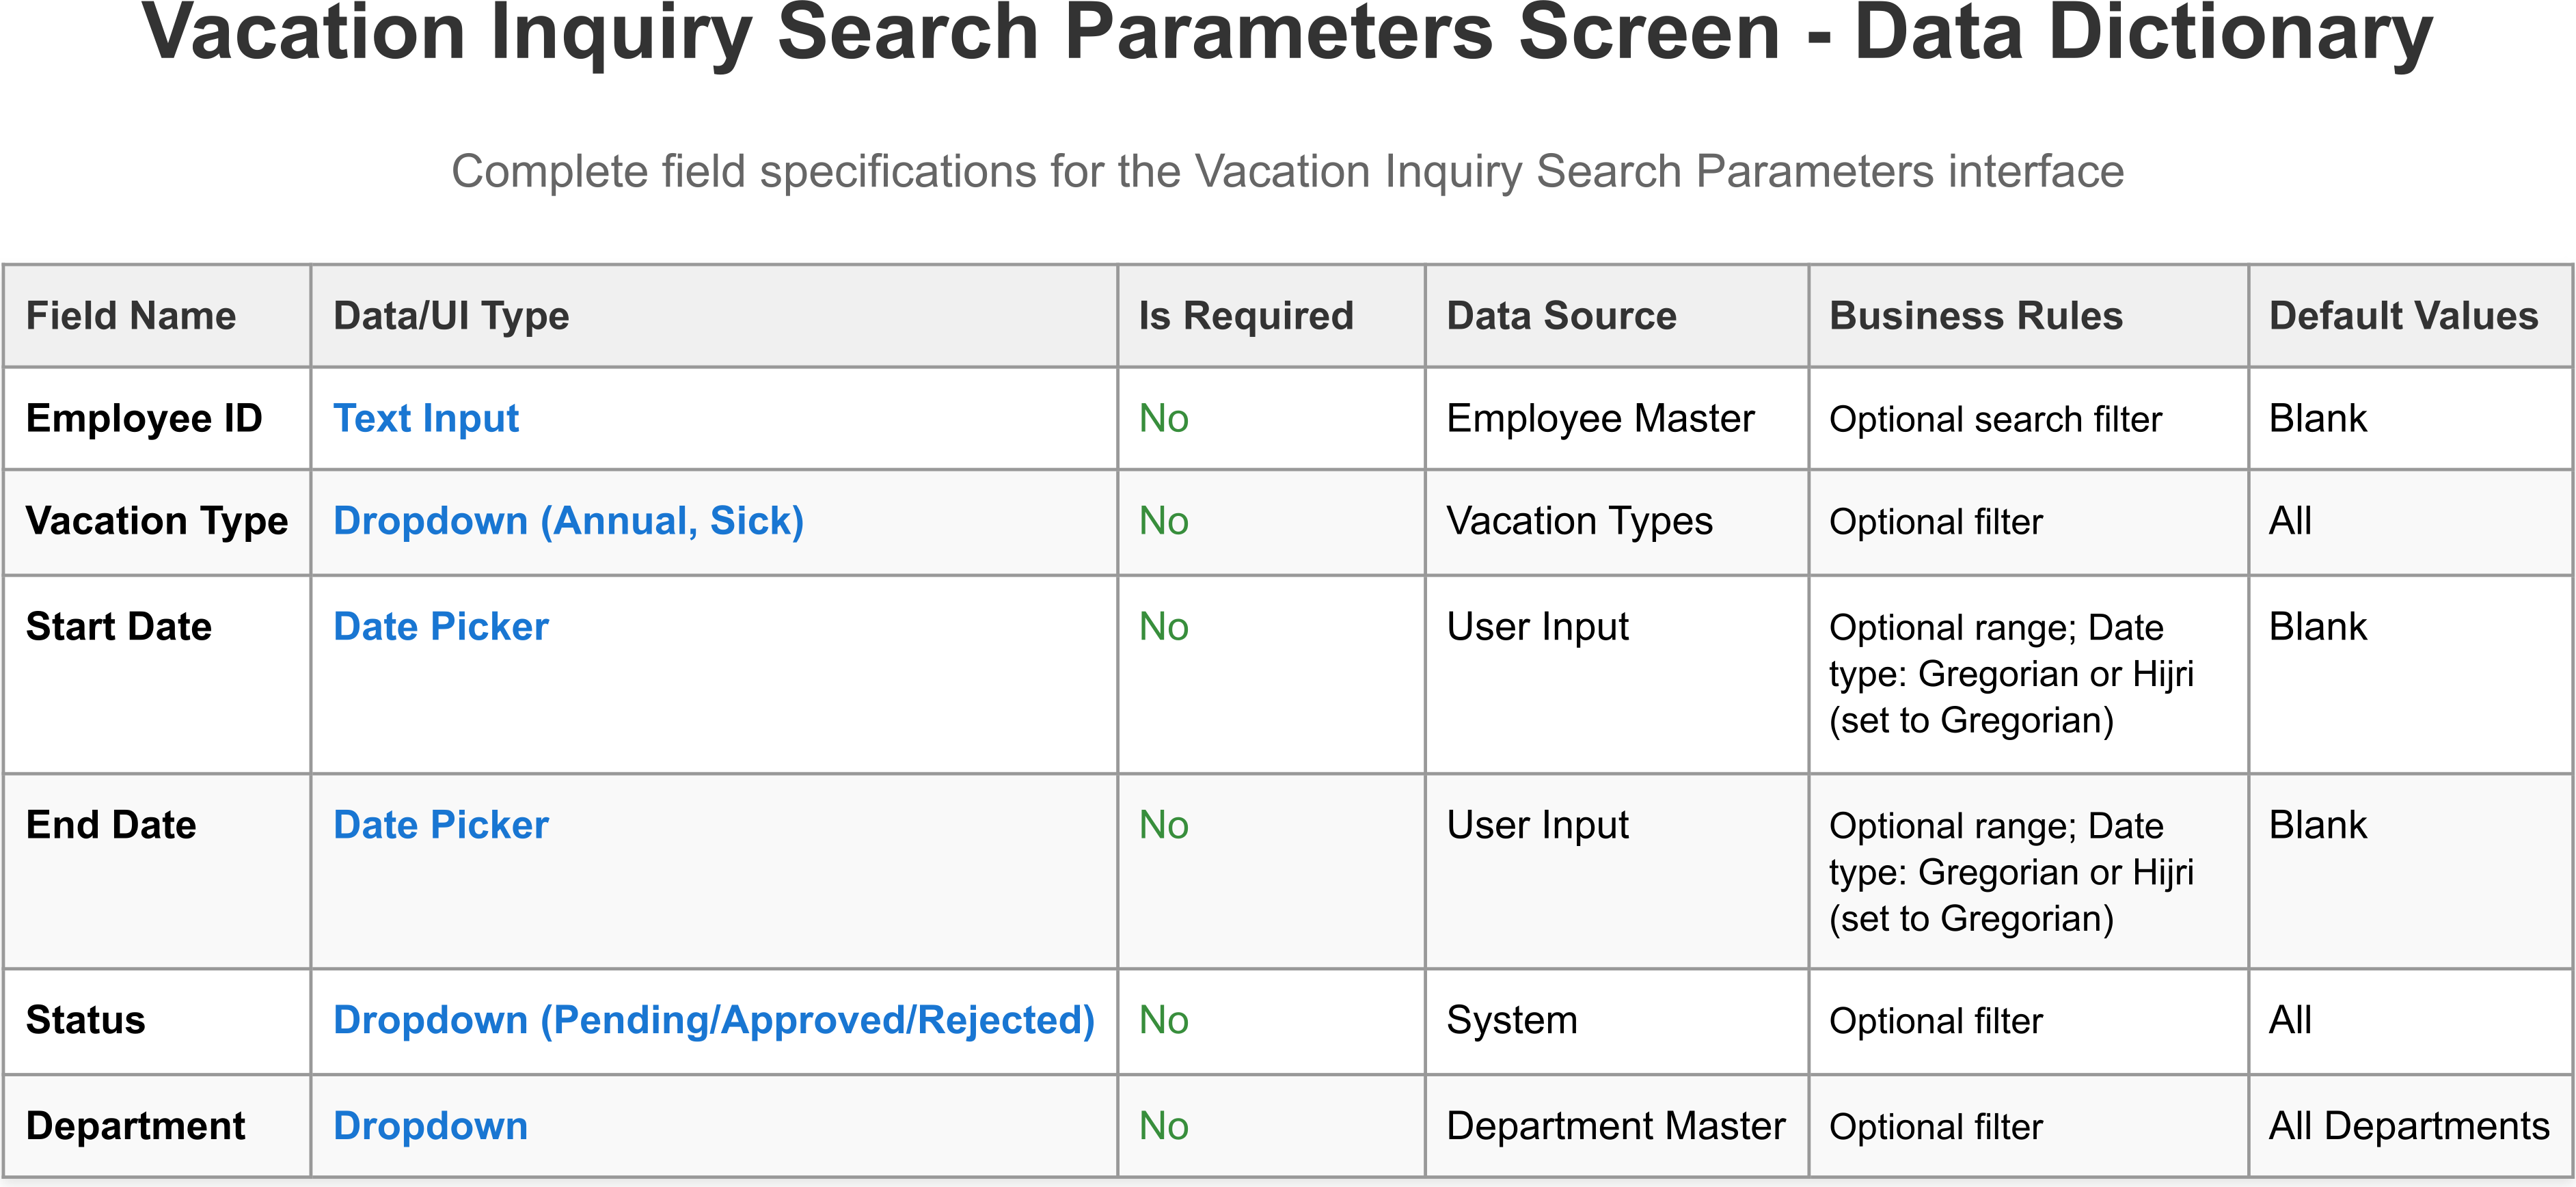
\includegraphics[width=0.9\textwidth]{Data-Dictionary/Screen-Data-Dictionaries/Vacation-Inquiry-Search-Parameters-Screen-Data-Dictionary/Vacation-Inquiry-Search-Parameters-Screen-Data-Dictionary-1.png}
\caption{Vacation Inquiry Search Parameters Screen Data Dictionary}
\label{fig:inquiry-search-params-data-dict}
\end{figure}

\subsubsection{Vacation Inquiry Search Results Screen Data Dictionary}
\begin{figure}[H]
\centering
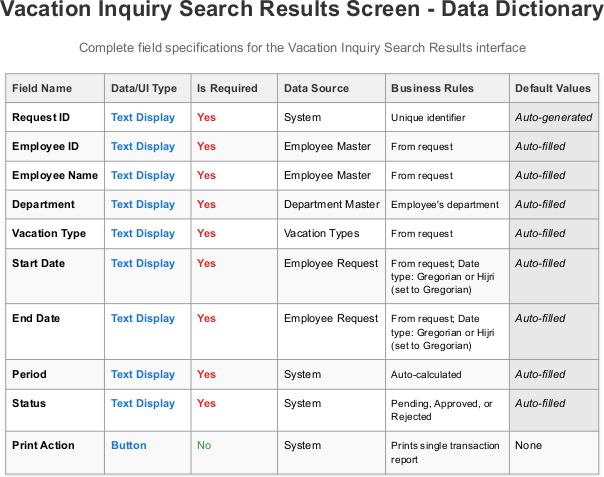
\includegraphics[width=0.9\textwidth]{Data-Dictionary/Screen-Data-Dictionaries/Vacation-Inquiry-Search-Results-Screen-Data-Dictionary/Vacation-Inquiry-Search-Results-Screen-Data-Dictionary-1.png}
\caption{Vacation Inquiry Search Results Screen Data Dictionary}
\label{fig:inquiry-search-results-data-dict}
\end{figure}

\subsubsection{Notifications Center Screen Data Dictionary}
\begin{figure}[H]
\centering
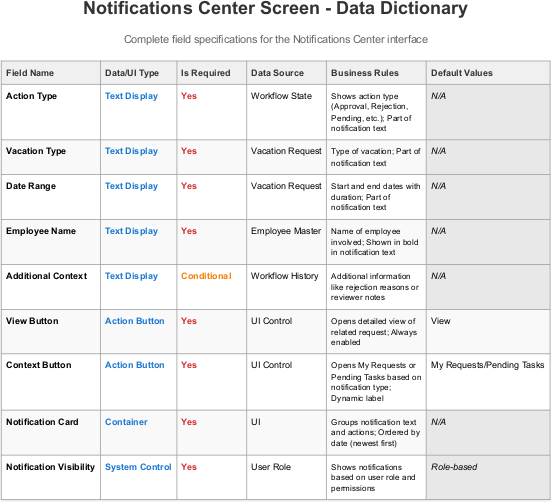
\includegraphics[width=0.9\textwidth]{Data-Dictionary/Screen-Data-Dictionaries/Notifications-Center-Screen-Data-Dictionary/Notifications-Center-Screen-Data-Dictionary-1.png}
\caption{Notifications Center Screen Data Dictionary}
\label{fig:notifications-center-data-dict}
\end{figure}

\subsubsection{Print Single Transaction Report Data Dictionary}
\begin{figure}[H]
\centering
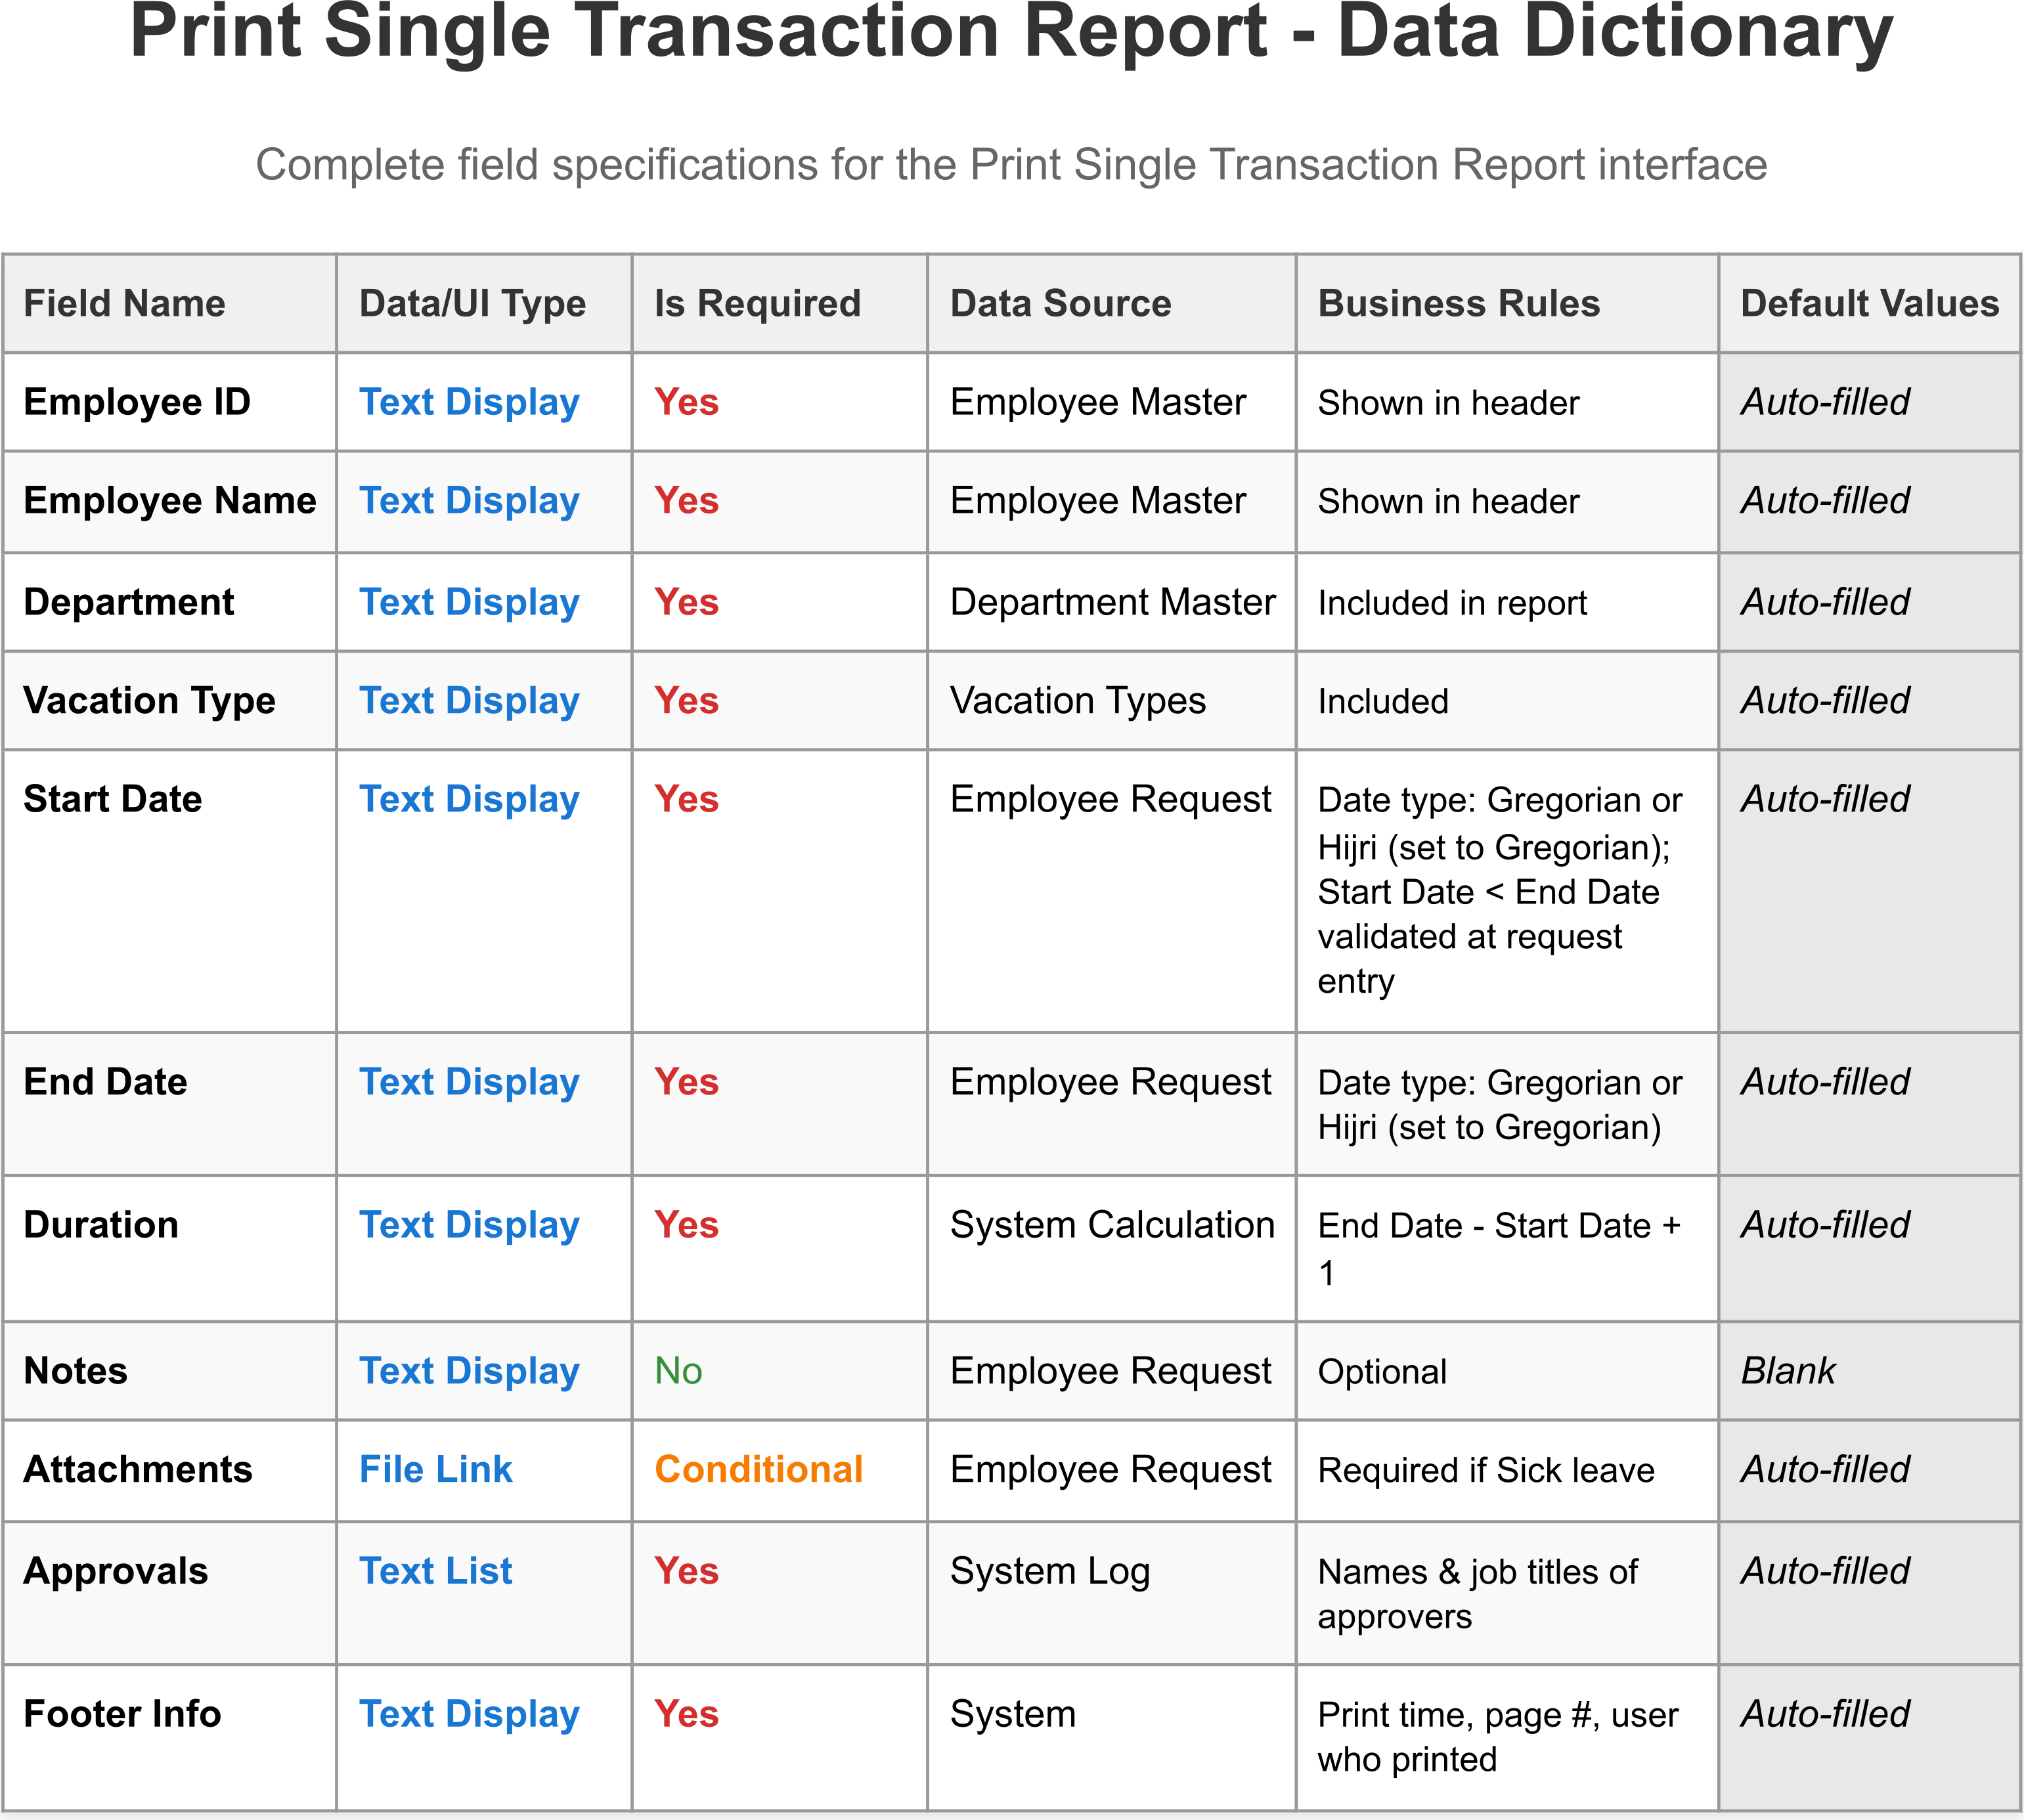
\includegraphics[width=0.9\textwidth]{Data-Dictionary/Screen-Data-Dictionaries/Print-Single-Transaction-Report-Data-Dictionary/Print-Single-Transaction-Report-Data-Dictionary-1.png}
\caption{Print Single Transaction Report Data Dictionary}
\label{fig:print-single-transaction-data-dict}
\end{figure}

\subsubsection{Print Comparative Annual Report Data Dictionary}
\begin{figure}[H]
\centering
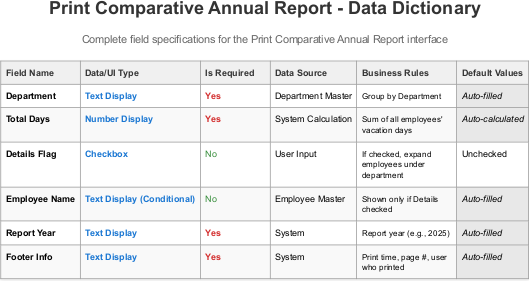
\includegraphics[width=0.9\textwidth]{Data-Dictionary/Screen-Data-Dictionaries/Print-Comparative-Annual-Report-Data-Dictionary/Print-Comparative-Annual-Report-Data-Dictionary-1.png}
\caption{Print Comparative Annual Report Data Dictionary}
\label{fig:print-comparative-annual-data-dict}
\end{figure}

\section{System Messages}

The system includes a comprehensive message table for all user communications and error messages. This table defines the content, context, and display rules for system-generated messages.

\subsection{System Messages Table}
The following images show the complete system messages table:

\begin{figure}[H]
\centering
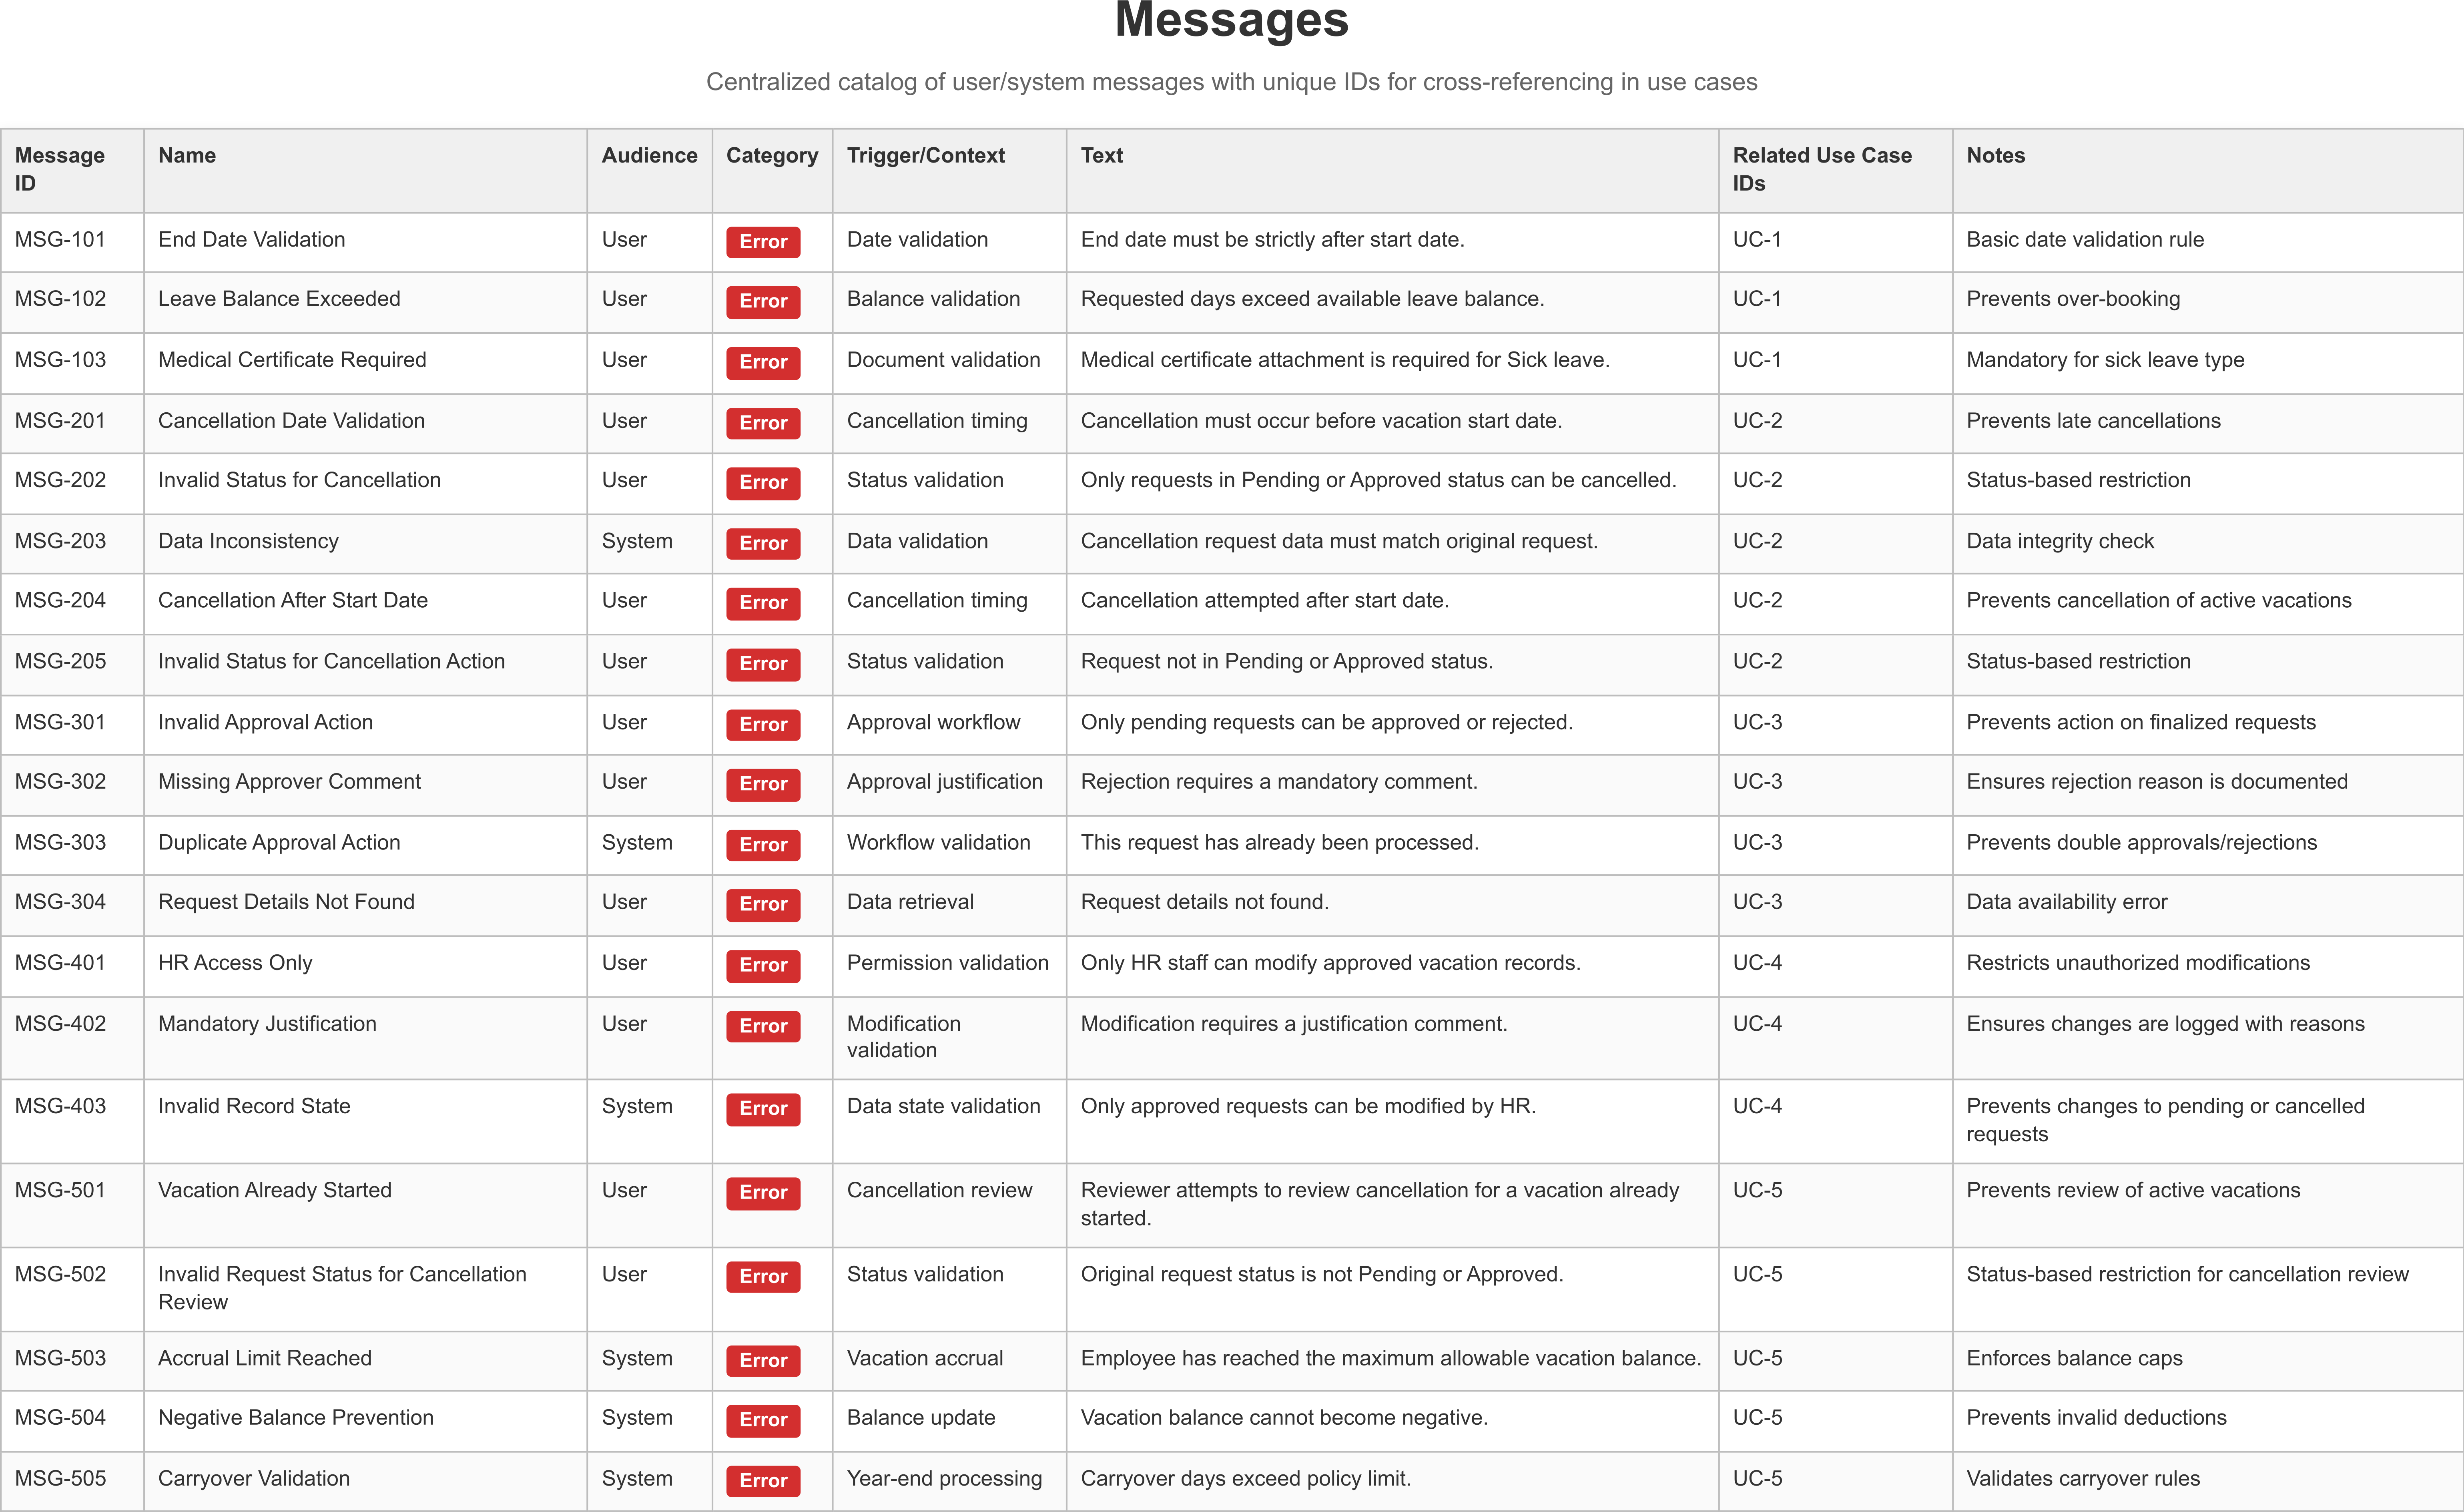
\includegraphics[width=1.0\textwidth]{Use-Cases/Messages-Table/Messages-Table-1.png}
\caption{System Messages Table - Part 1}
\label{fig:messages-table-1}
\end{figure}

\begin{figure}[H]
\centering
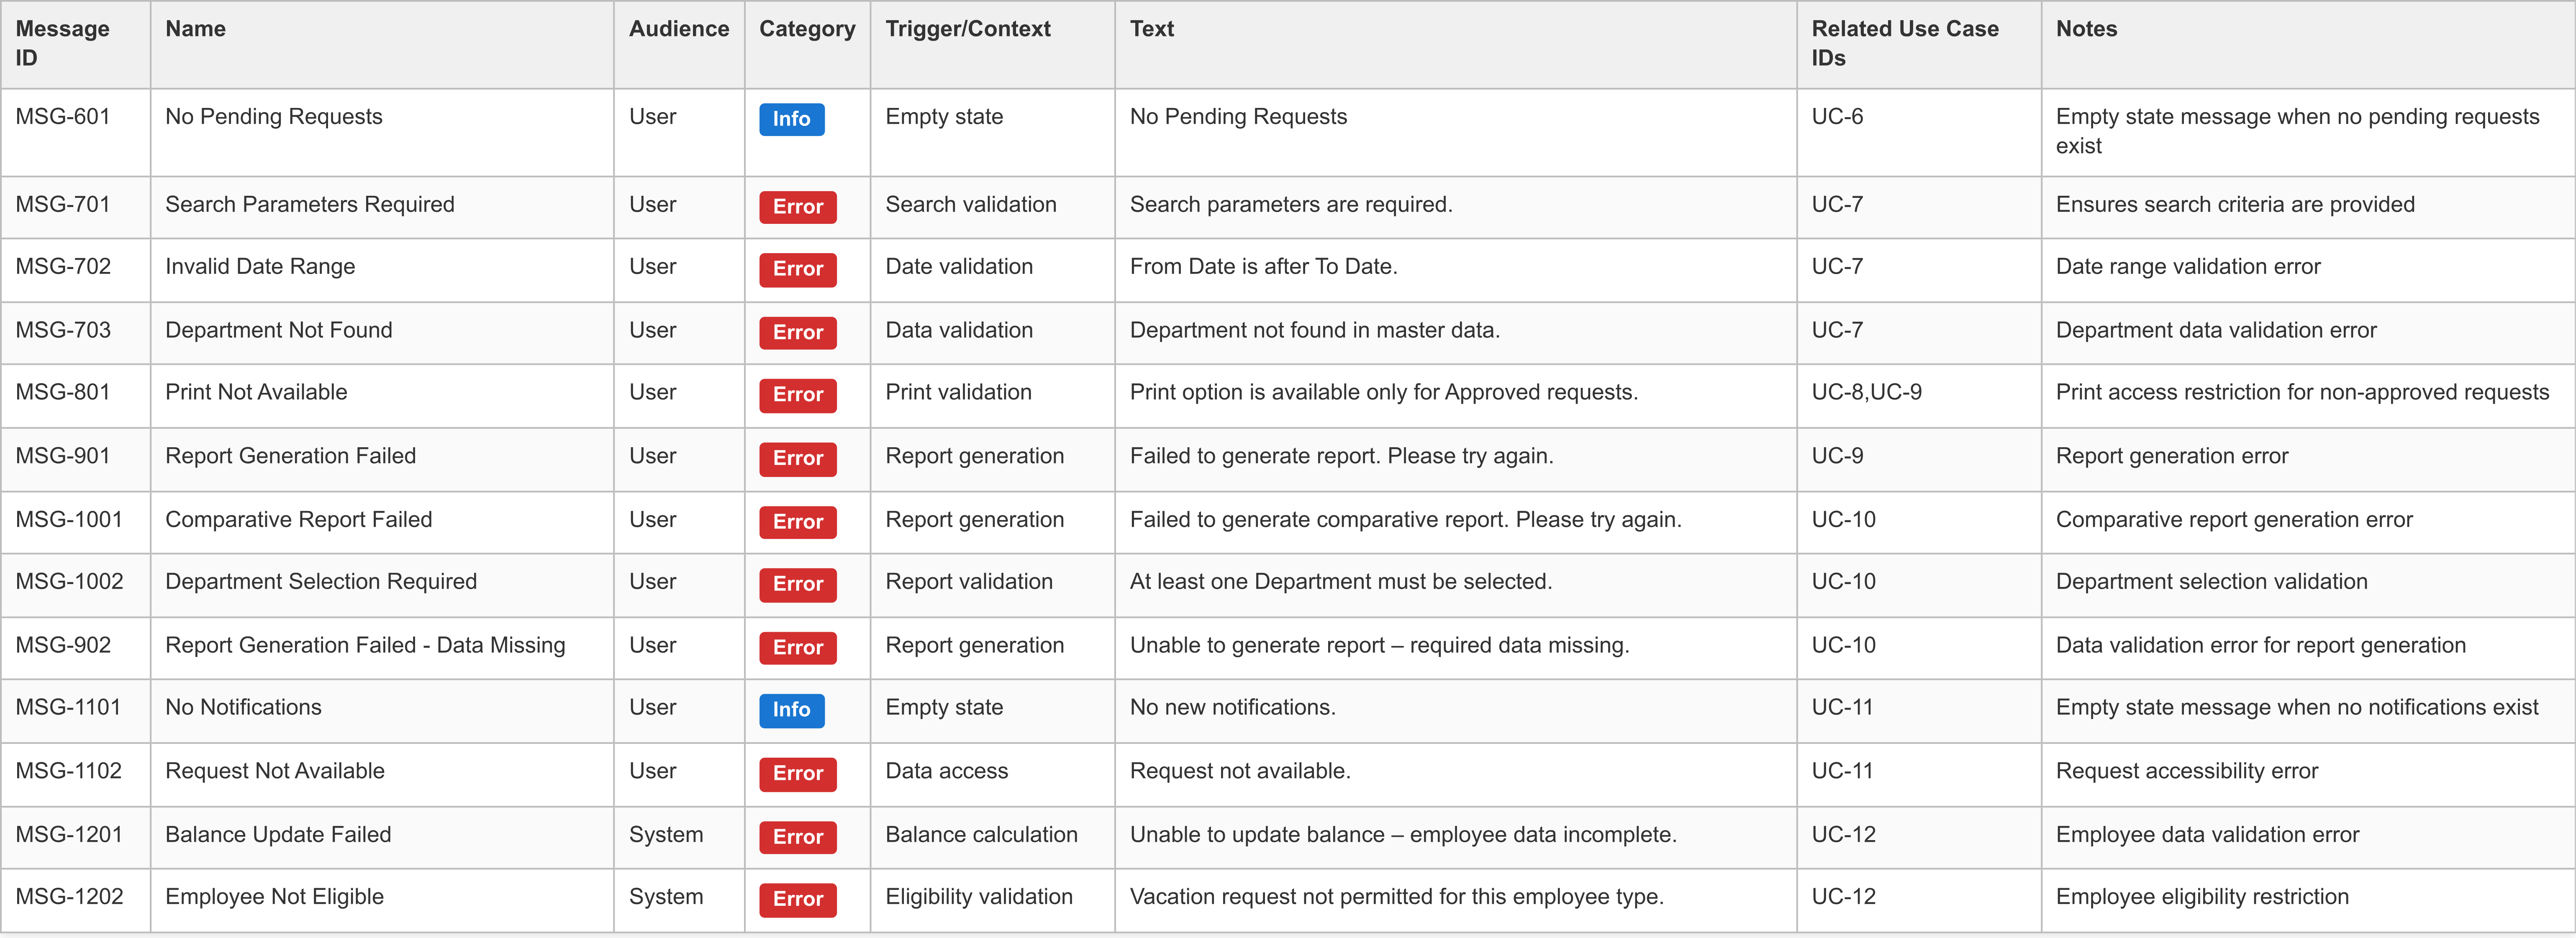
\includegraphics[width=1.0\textwidth]{Use-Cases/Messages-Table/Messages-Table-2.png}
\caption{System Messages Table - Part 2}
\label{fig:messages-table-2}
\end{figure}

\subsection{Message Categories}
\begin{itemize}
    \item \textbf{Validation Messages}: Field validation errors and business rule violations
    \item \textbf{Workflow Messages}: Approval status updates and workflow progression
    \item \textbf{Notification Messages}: System notifications and user alerts
    \item \textbf{Error Messages}: System errors and exception handling
    \item \textbf{Success Messages}: Confirmation of successful operations
\end{itemize}

\section{Appendices}

\subsection{Appendix A: Glossary}
\begin{itemize}
    \item \textbf{Vacation}: Time off from work for personal reasons
    \item \textbf{Leave Balance}: Remaining vacation days available
    \item \textbf{Approval Workflow}: Process for request authorization
    \item \textbf{Escalation}: Automatic forwarding of delayed requests
    \item \textbf{Attachments}: Supporting documents for requests
    \item \textbf{Entitlement}: Annual vacation days allocation
    \item \textbf{Trainee}: Employee in training status, ineligible for vacation
    \item \textbf{Business Rule}: System behavior rule that governs functionality
    \item \textbf{Use Case}: Specific interaction scenario between users and system
\end{itemize}

\subsection{Appendix B: Data Models}
\begin{itemize}
    \item Entity-Relationship Diagrams
    \item Database Schema Definitions
    \item API Specification Documents
    \item Integration Interface Definitions
    \item Master Data Entity Definitions
\end{itemize}

\subsection{Appendix B.1: Data Dictionary Template}
The following image shows the standard data dictionary template used for documenting all system data entities:

\begin{figure}[H]
\centering
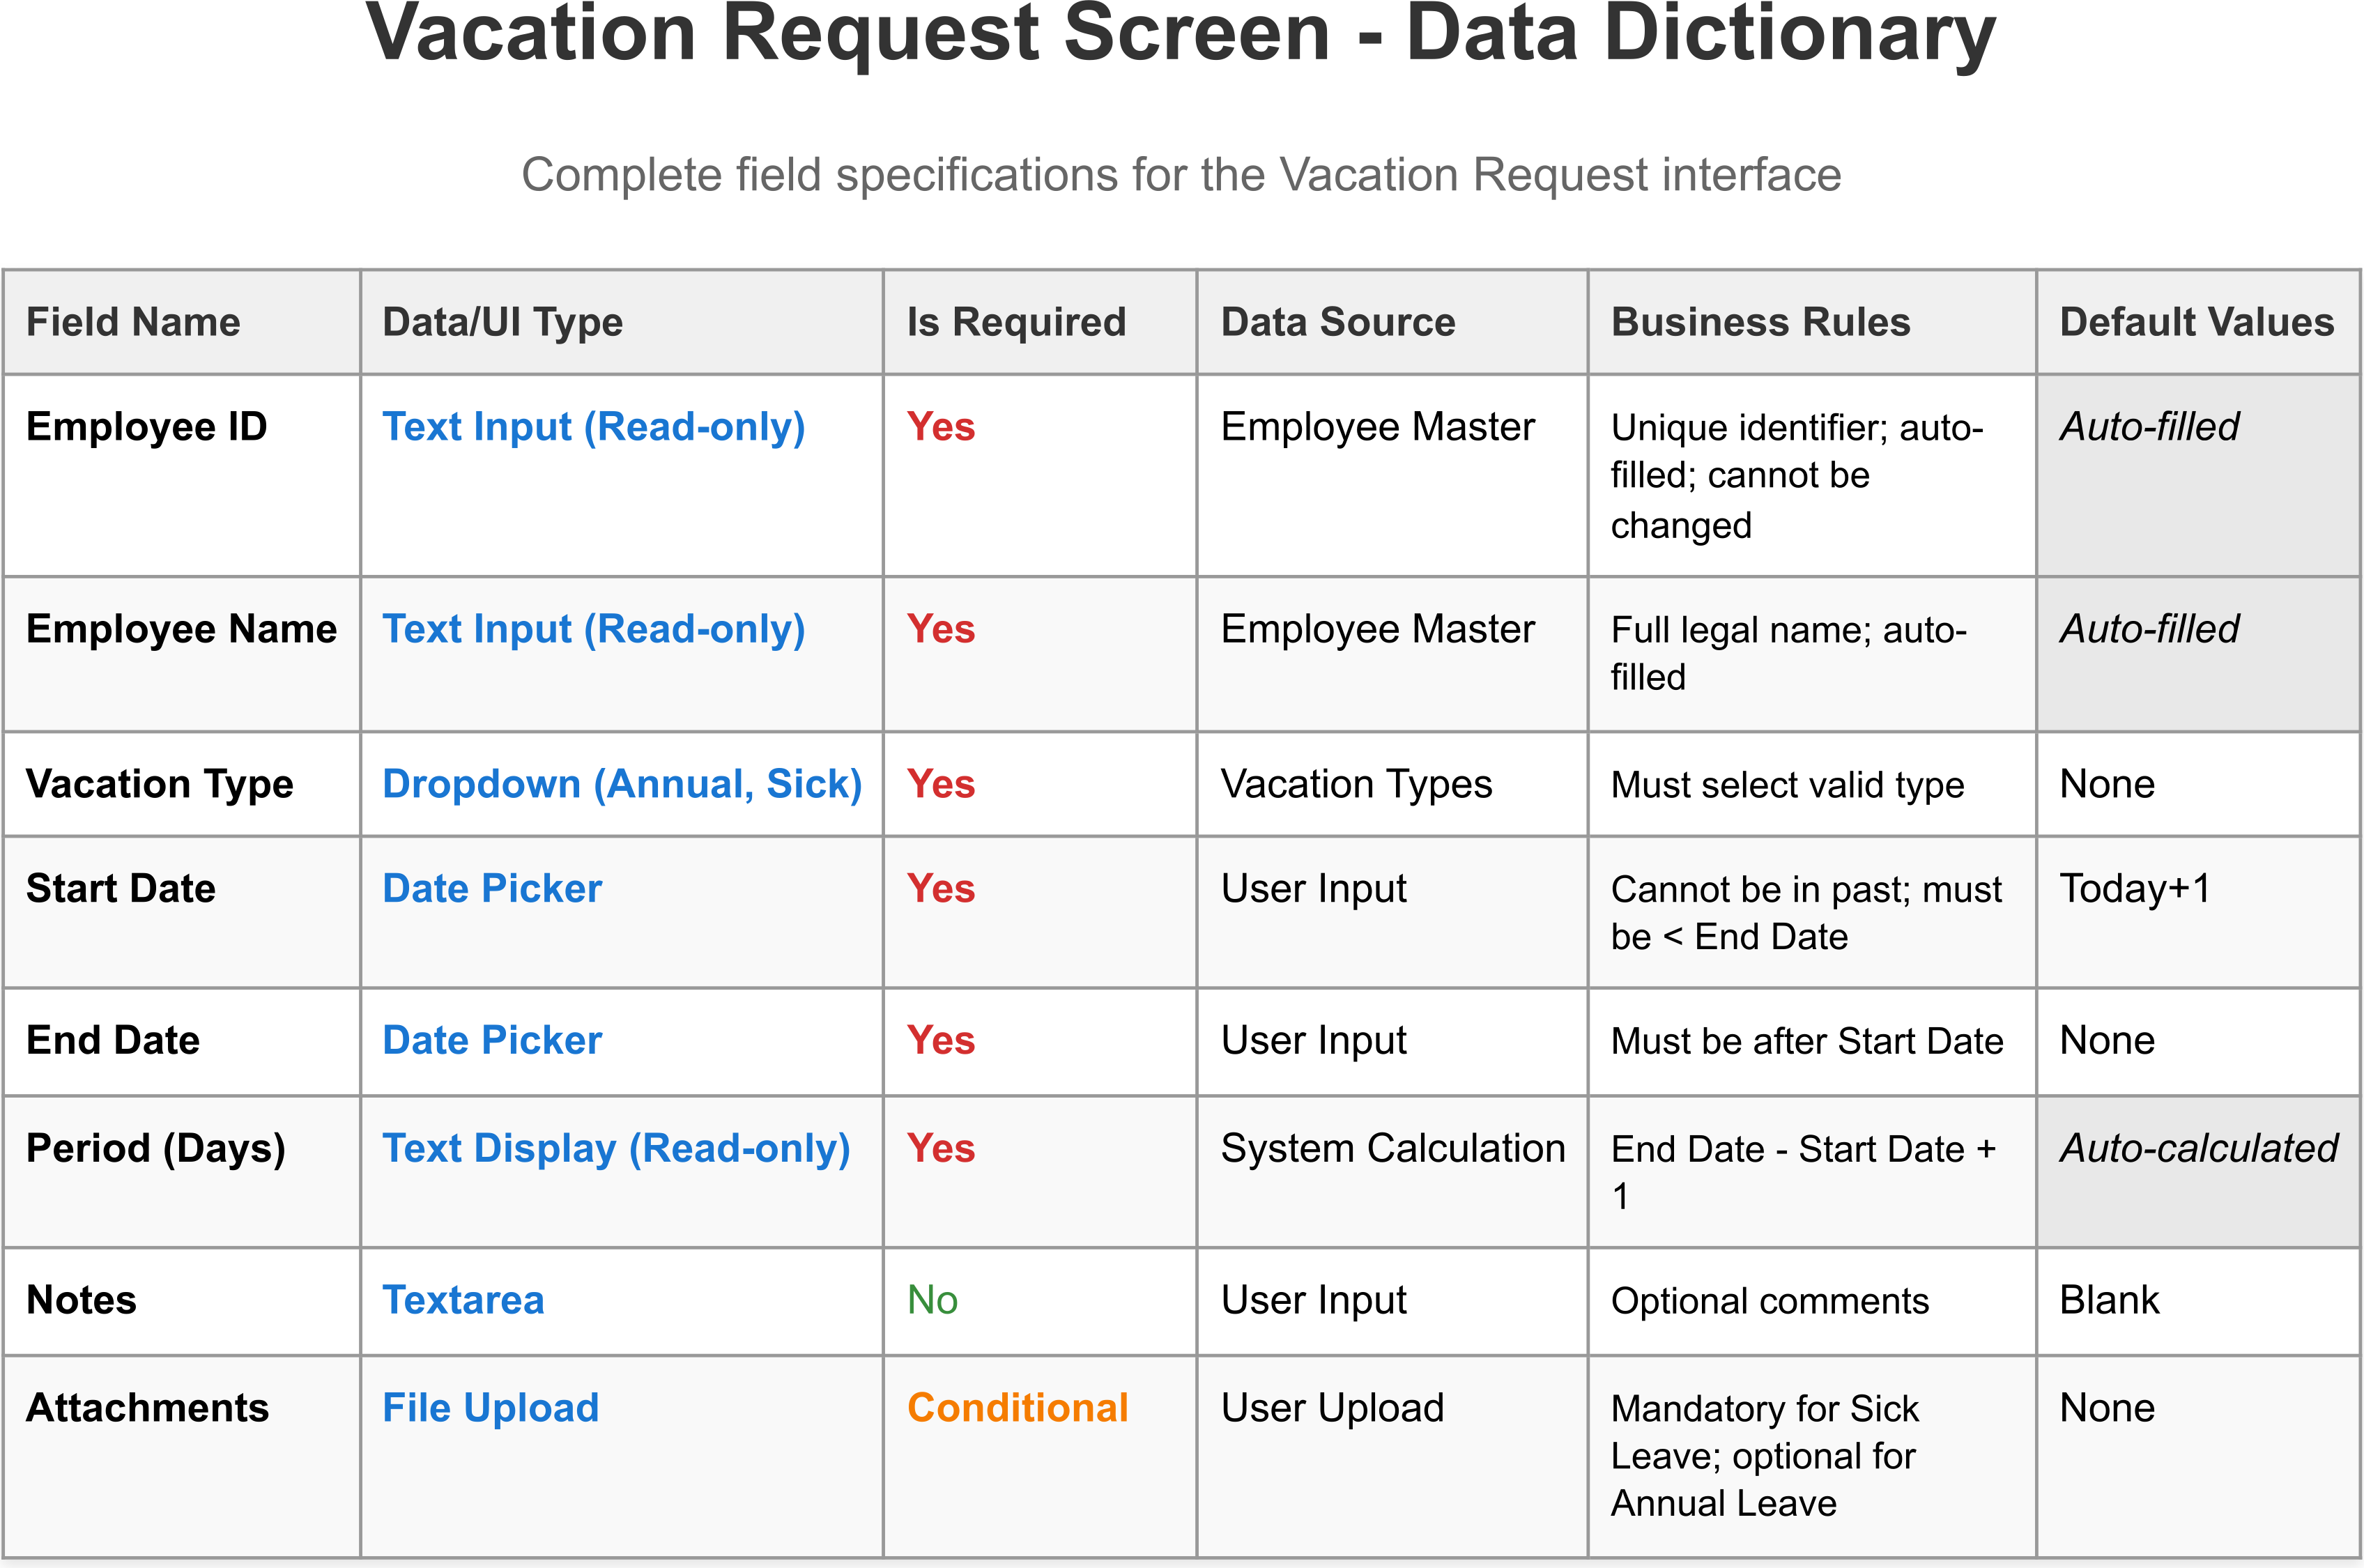
\includegraphics[width=0.9\textwidth]{Data-Dictionary/Data-Dictionary-Template/Data-Dictionary-Template-1.png}
\caption{Data Dictionary Template}
\label{fig:data-dictionary-template}
\end{figure}

\subsection{Appendix C: Wireframe Images}
This section contains all the wireframe images for the system's user interfaces:

\subsubsection{Core Application Screens}

\paragraph{Vacation Request Screen}
\begin{figure}[H]
\centering
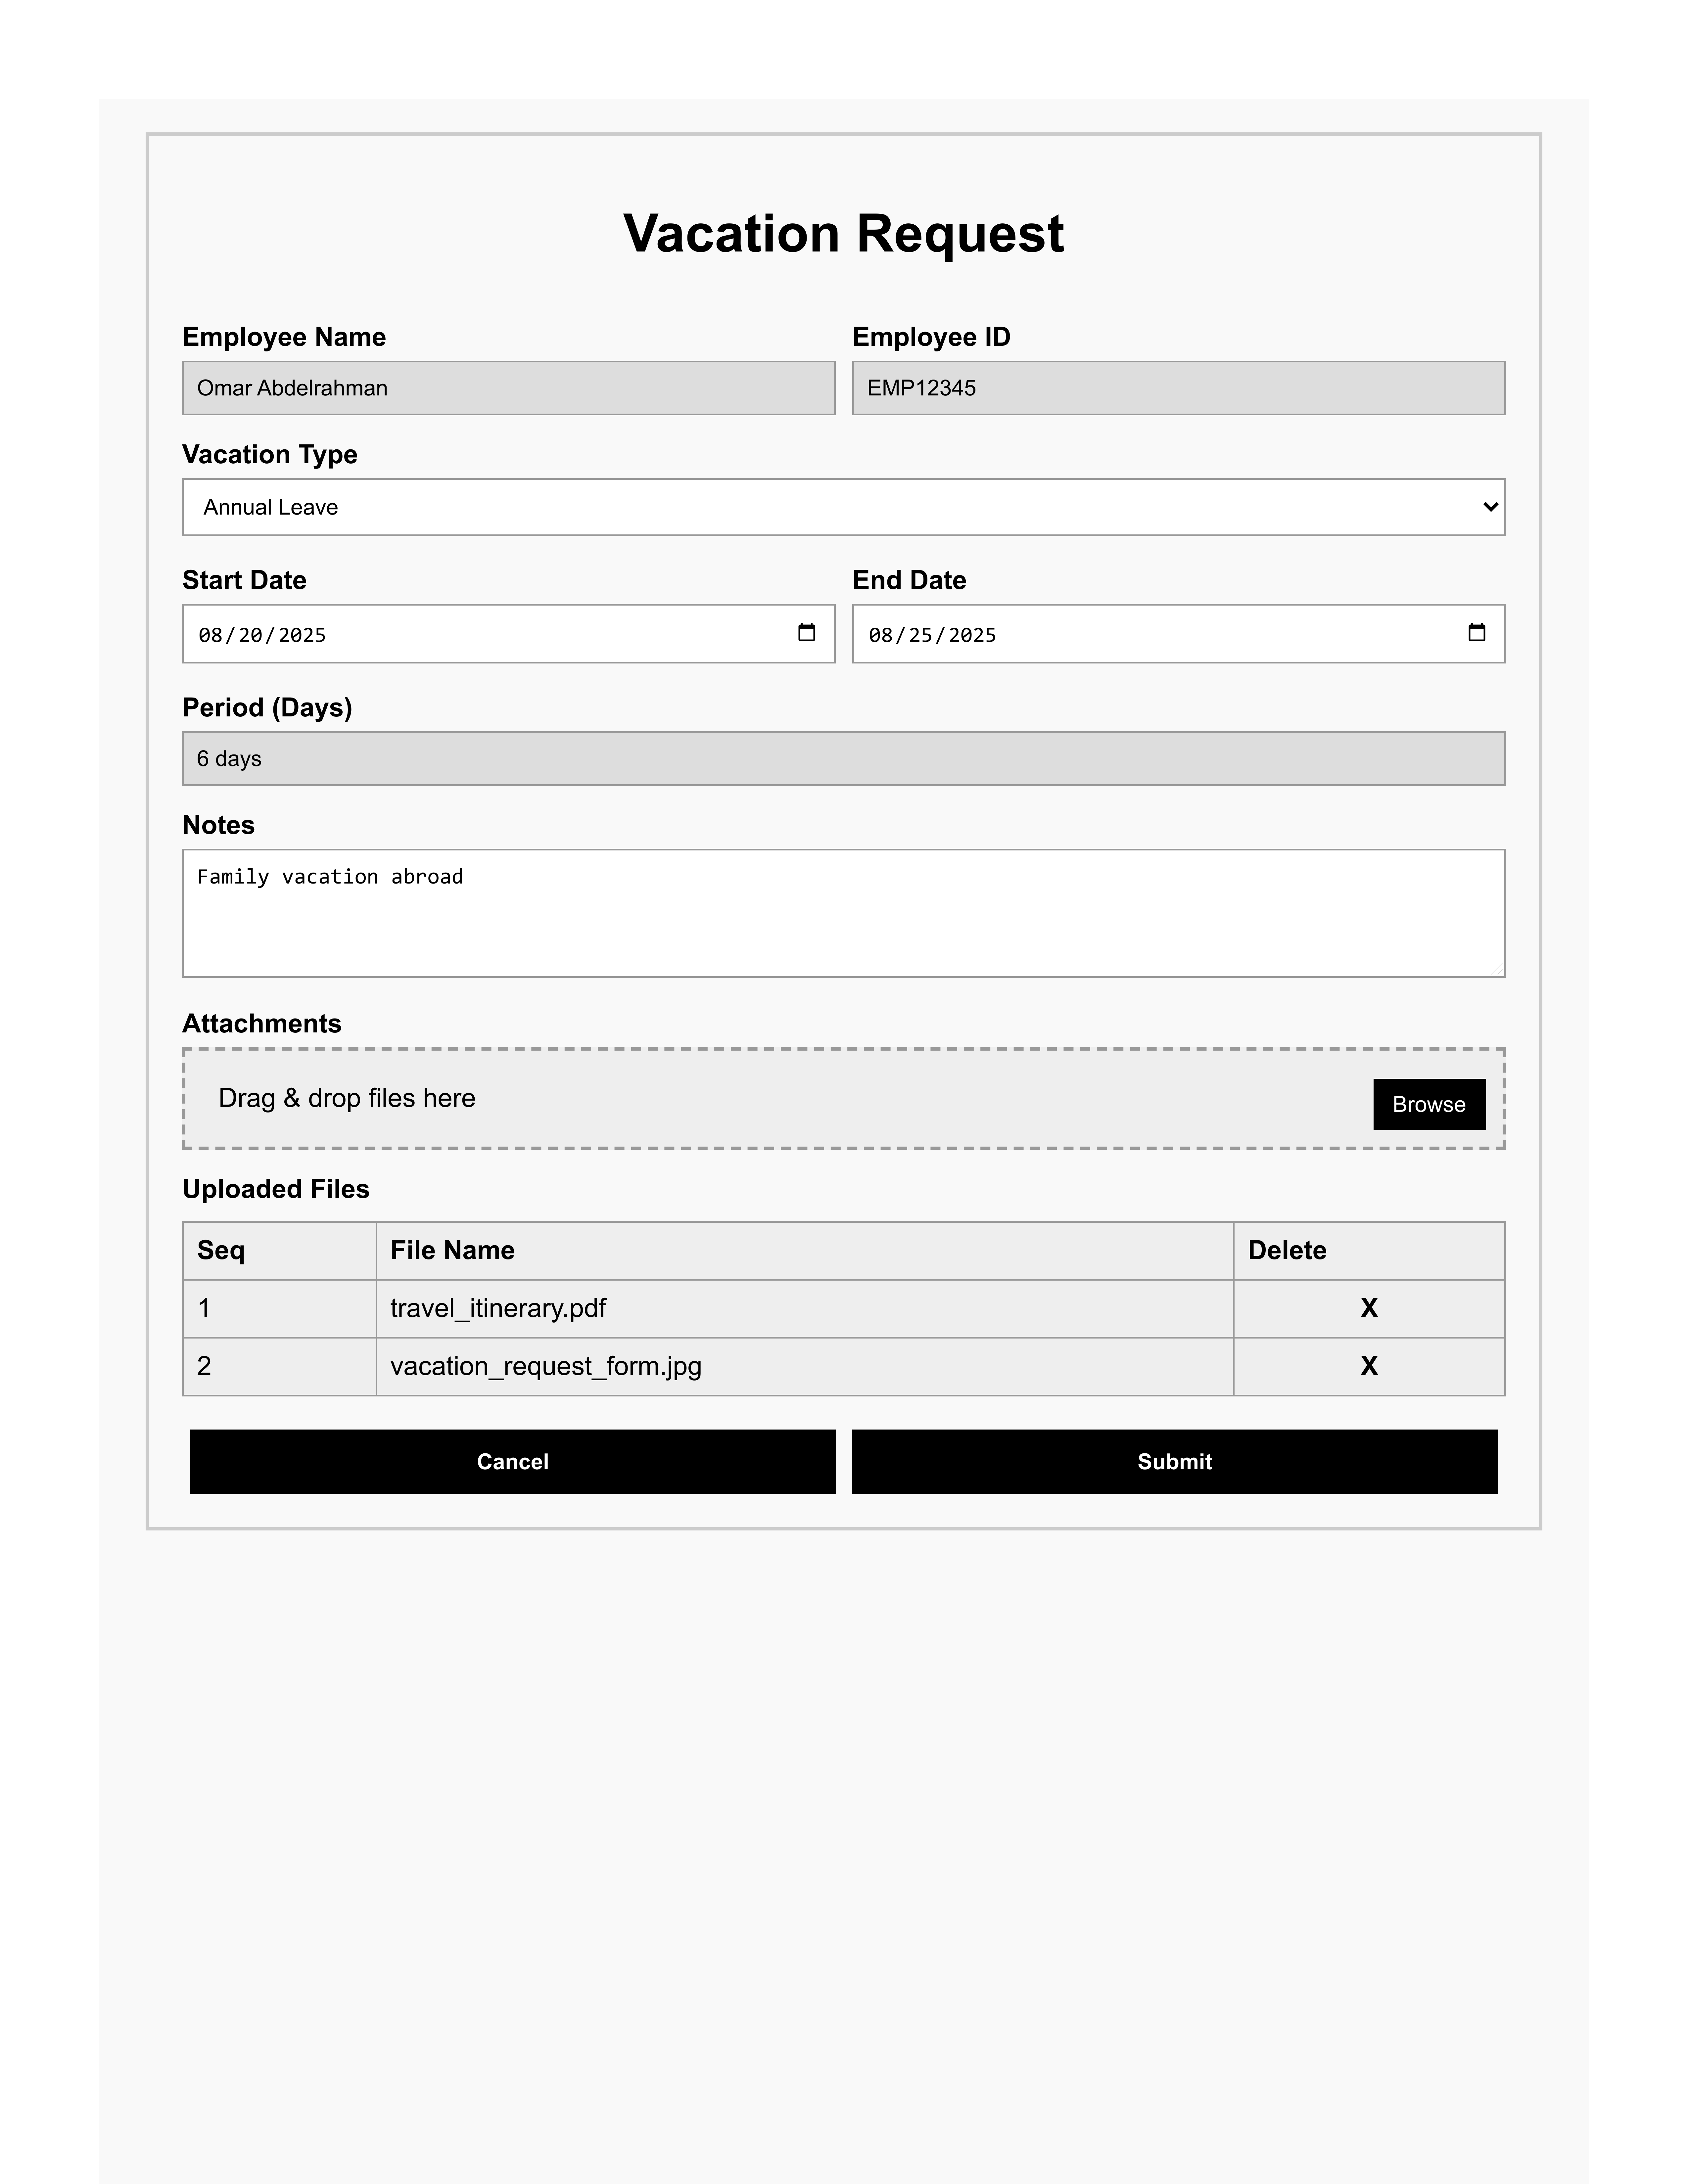
\includegraphics[width=0.8\textwidth]{Wireframes/Vacation-Request/Vacation-Request-1.png}
\caption{Vacation Request Screen Wireframe}
\label{fig:wireframe-vacation-request}
\end{figure}

\paragraph{Vacation Cancellation Request Screen}
\begin{figure}[H]
\centering
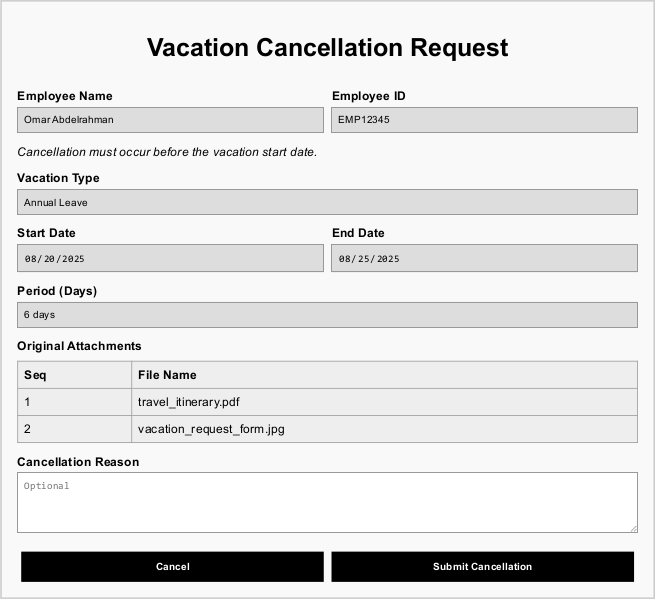
\includegraphics[width=0.8\textwidth]{Wireframes/Vacation-Cancellation-Request/Vacation-Cancellation-Request-1.png}
\caption{Vacation Cancellation Request Screen Wireframe}
\label{fig:wireframe-vacation-cancellation}
\end{figure}

\paragraph{Review Vacation Request Screen}
\begin{figure}[H]
\centering
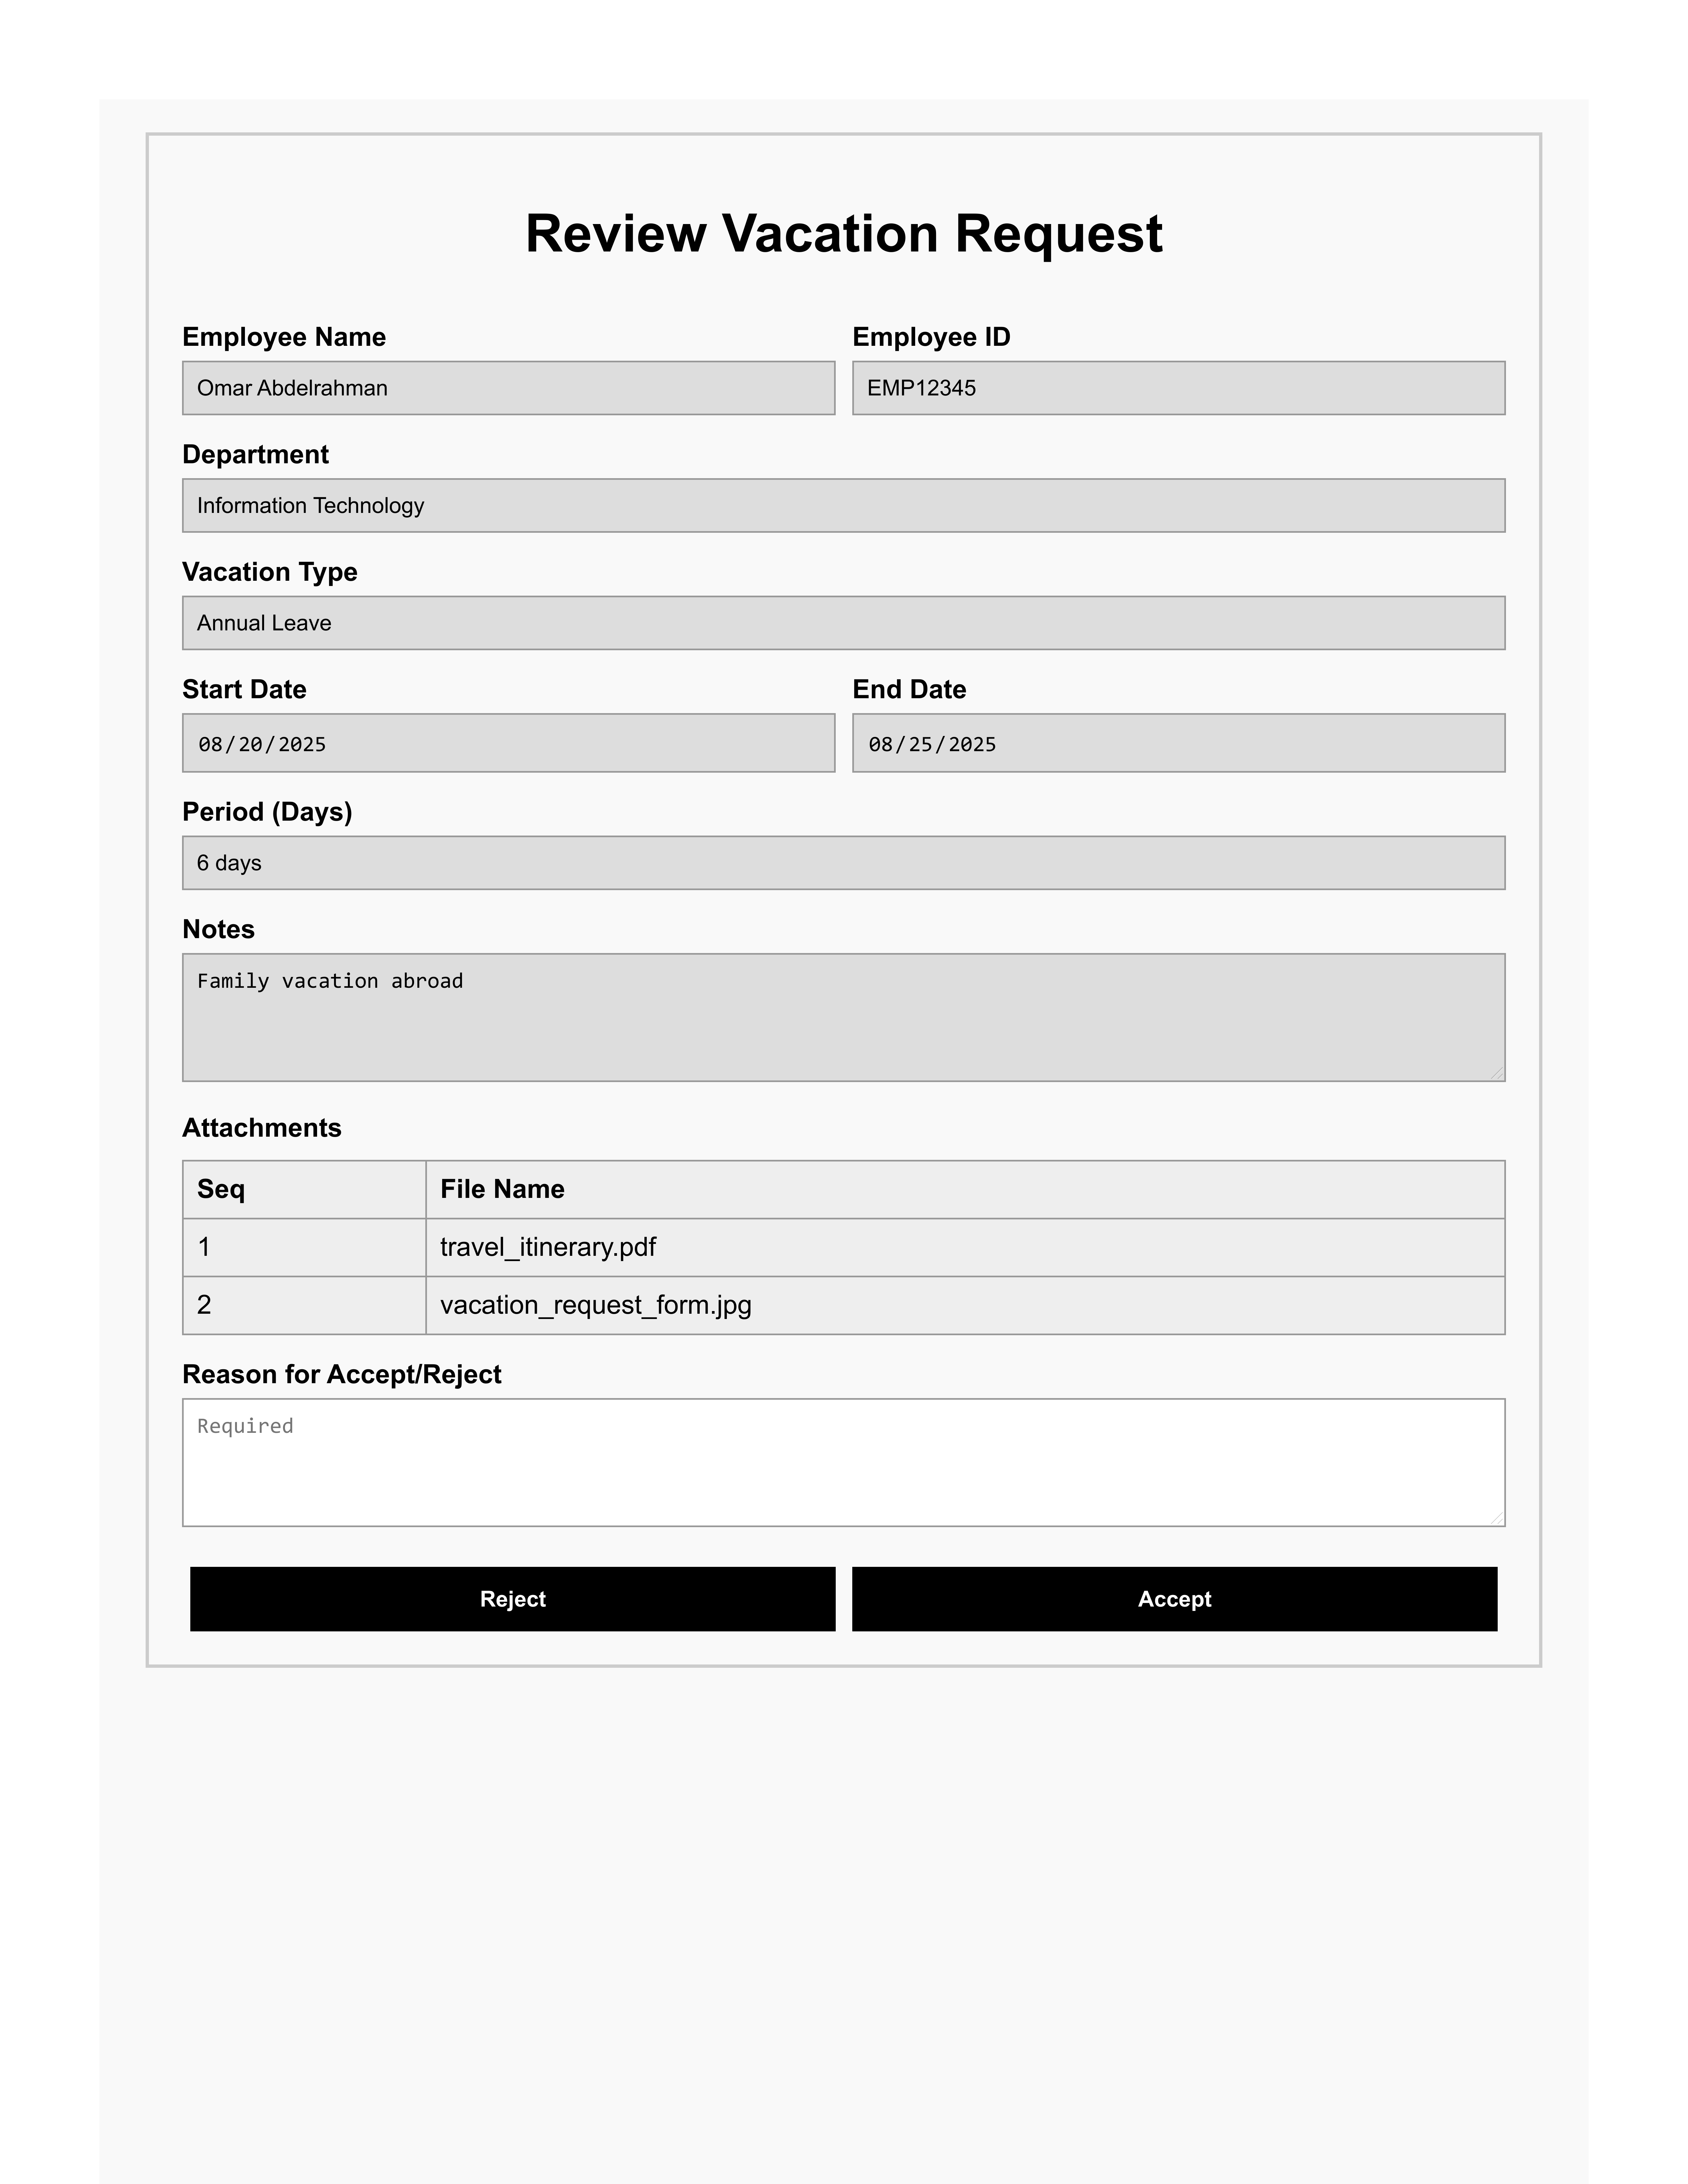
\includegraphics[width=0.8\textwidth]{Wireframes/Review-Vacation-Request/Review-Vacation-Request-1.png}
\caption{Review Vacation Request Screen Wireframe}
\label{fig:wireframe-review-vacation}
\end{figure}

\paragraph{Review Vacation Cancellation Request Screen}
\begin{figure}[H]
\centering
\includegraphics[width=0.8\textwidth]{Wireframes/Review-Vacation-Cancellation-Request/Review-Vacation-Cancellation-Request-1.png}
\caption{Review Vacation Cancellation Request Screen Wireframe}
\label{fig:wireframe-review-cancellation}
\end{figure}

\paragraph{My Vacation Requests Screen}
\begin{figure}[H]
\centering
\includegraphics[width=0.8\textwidth]{Wireframes/My-Vacation-Requests/My-Vacation-Requests-1.png}
\caption{My Vacation Requests Screen Wireframe}
\label{fig:wireframe-my-vacation-requests}
\end{figure}

\paragraph{Pending Vacation Requests Screen}
\begin{figure}[H]
\centering
\includegraphics[width=0.8\textwidth]{Wireframes/Pending-Vacation-Requests/Pending-Vacation-Requests-1.png}
\caption{Pending Vacation Requests Screen Wireframe}
\label{fig:wireframe-pending-vacation-requests}
\end{figure}

\paragraph{Vacation Inquiry Search Parameters Screen}
\begin{figure}[H]
\centering
\includegraphics[width=0.8\textwidth]{Wireframes/Employee-Vacation-Inquiry-Search-Parameters/Employee-Vacation-Inquiry-Search-Parameters-1.png}
\caption{Vacation Inquiry Search Parameters Screen Wireframe}
\label{fig:wireframe-inquiry-search-params}
\end{figure}

\paragraph{Vacation Inquiry Search Results Screen}
\begin{figure}[H]
\centering
\includegraphics[width=0.8\textwidth]{Wireframes/Employee-Vacation-Inquiry-Search-Results/Employee-Vacation-Inquiry-Search-Results-1.png}
\caption{Vacation Inquiry Search Results Screen Wireframe}
\label{fig:wireframe-inquiry-search-results}
\end{figure}

\paragraph{Notifications Center Screen}
\begin{figure}[H]
\centering
\includegraphics[width=0.8\textwidth]{Wireframes/Notifications-Center/Notifications-Center-1.png}
\caption{Notifications Center Screen Wireframe}
\label{fig:wireframe-notifications-center}
\end{figure}

\paragraph{Requests Center Screen}
\begin{figure}[H]
\centering
\includegraphics[width=0.8\textwidth]{Wireframes/Requests-Center/Requests-Center-1.png}
\caption{Requests Center Screen Wireframe}
\label{fig:wireframe-requests-center}
\end{figure}

\subsubsection{Report Layout Screens}

\paragraph{Single Transaction Report Layout}
\begin{figure}[H]
\centering
\includegraphics[width=0.8\textwidth]{Wireframes/Print-Layout-Single-Transaction-Report/Print-Layout-Single-Transaction-Report-1.png}
\caption{Single Transaction Report Layout Wireframe}
\label{fig:wireframe-single-transaction-report}
\end{figure}

\paragraph{Annual Comparative Report Layout}
\begin{figure}[H]
\centering
\includegraphics[width=0.8\textwidth]{Wireframes/Print-Layout-Annual-Comparative-Report/Print-Layout-Annual-Comparative-Report-Web-1.png}
\caption{Annual Comparative Report Layout Wireframe}
\label{fig:wireframe-annual-comparative-report}
\end{figure}

\paragraph{Annual Comparative Report Search Parameters}
\begin{figure}[H]
\centering
\includegraphics[width=0.8\textwidth]{Wireframes/Annual-Comparative-Report-Search-Parameters/Annual-Comparative-Report-Search-Parameters-1.png}
\caption{Annual Comparative Report Search Parameters Wireframe}
\label{fig:wireframe-annual-comparative-report-search-params}
\end{figure}

\subsection{Appendix D: State Diagrams}
The system implements comprehensive state management for vacation requests and workflows:

\begin{figure}[H]
\centering
\includegraphics[width=0.9\textwidth]{Diagrams/State-Diagram/State-Diagram.png}
\caption{Vacation Request State Diagram}
\label{fig:state-diagram}
\end{figure}

\subsection{Appendix E: Workflow Diagrams}
The system implements several key workflow processes:

\subsubsection{Basic Vacation Request Flow}
\begin{figure}[H]
\centering
\includegraphics[width=0.8\textwidth]{Diagrams/Workflows/Vacation-Request-Basic-Flow/Vacation-Request-Basic-Flow.png}
\caption{Basic Vacation Request Workflow}
\label{fig:basic-flow}
\end{figure}

\subsubsection{Escalation to Sponsor Flow}
\begin{figure}[H]
\centering
\includegraphics[width=0.8\textwidth]{Diagrams/Workflows/Vacation-Request-Escalation-to-Sponsor/Vacation-Request-Escalation-to-Sponsor.png}
\caption{Vacation Request Escalation to Sponsor Workflow}
\label{fig:escalation-flow}
\end{figure}

\subsubsection{Resubmission After Rejection Flow}
\begin{figure}[H]
\centering
\includegraphics[width=0.8\textwidth]{Diagrams/Workflows/Vacation-Request-Resubmission-After-Rejection/Vacation-Request-Resubmission-After-Rejection.png}
\caption{Vacation Request Resubmission After Rejection Workflow}
\label{fig:resubmission-flow}
\end{figure}

\subsection{Appendix F: Use Case Templates}
The following image shows the standard use case template used for documenting all system use cases:

\begin{figure}[H]
\centering
\includegraphics[width=0.9\textwidth]{Use-Cases/Use-Case-Template/Use-Case-Template-1.png}
\caption{Use Case Template}
\label{fig:use-case-template}
\end{figure}

For complete use case specifications, refer to the All-UseCases.json document. This document contains:

\begin{itemize}
    \item Standard Use Case Template
    \item Use Case Documentation Standards
    \item Business Rule Definition Format
    \item Exception Handling Documentation
    \item Complete specifications for all 12 use cases
\end{itemize}

\subsection{Appendix G: System Architecture \& Context}
The system architecture details are now presented in Section 3: System Architecture and Context for better contextual understanding. This appendix contains additional technical implementation details that complement the main architecture section.

\subsection{Appendix H: Technical Specifications}
This appendix contains technical implementation details that are typically covered in a System Design Document:

\subsubsection{Technology Stack}
\begin{itemize}
    \item \textbf{Frontend}: HTML5, CSS3, JavaScript, React/Angular
    \item \textbf{Backend}: Node.js/Python/Java
    \item \textbf{Database}: SQL Server/MySQL/PostgreSQL
    \item \textbf{PDF Generation}: jsPDF, iText, or similar
    \item \textbf{Authentication}: JWT, OAuth, or session-based
    \item \textbf{Workflow Engine}: Custom implementation or BPMS
\end{itemize}

\subsubsection{Performance Specifications}
\begin{itemize}
    \item \textbf{Response Time}: < 3 seconds for page loads
    \item \textbf{Database Queries}: < 1 second for standard operations
    \item \textbf{PDF Generation}: < 5 seconds for standard reports
    \item \textbf{Concurrent Users}: Support for 100+ simultaneous users
    \item \textbf{File Upload}: Support for multiple file types and sizes
\end{itemize}

\subsubsection{Security Specifications}
\begin{itemize}
    \item \textbf{Encryption}: AES-256 for sensitive data
    \item \textbf{Password Policy}: Minimum 8 characters, complexity requirements
    \item \textbf{Session Management}: Secure session handling with timeout
    \item \textbf{Input Validation}: SQL injection and XSS prevention
    \item \textbf{File Security}: Secure file upload and storage
\end{itemize}

\subsection{Appendix I: Testing Requirements}
This appendix contains testing specifications that are typically covered in a Test Plan:

\subsubsection{Functional Testing}
\begin{itemize}
    \item \textbf{Unit Testing}: Individual component testing
    \item \textbf{Integration Testing}: Module interaction testing
    \item \textbf{System Testing}: End-to-end functionality testing
    \item \textbf{User Acceptance Testing}: Stakeholder validation
    \item \textbf{Workflow Testing}: Approval process validation
\end{itemize}

\subsubsection{Non-Functional Testing}
\begin{itemize}
    \item \textbf{Performance Testing}: Load and stress testing
    \item \textbf{Security Testing}: Vulnerability assessment
    \item \textbf{Usability Testing}: User experience validation
    \item \textbf{Compatibility Testing}: Cross-browser and device testing
    \item \textbf{PDF Generation Testing}: Report output validation
\end{itemize}

\subsection{Appendix J: Deployment and Maintenance}
This appendix contains deployment and maintenance specifications that are typically covered in a Project Plan:

\subsubsection{Deployment Strategy}
\begin{itemize}
    \item \textbf{Environment Setup}: Development, testing, production
    \item \textbf{Database Migration}: Schema creation and data migration
    \item \textbf{User Training}: Comprehensive training program
    \item \textbf{Go-Live Plan}: Phased rollout strategy
    \item \textbf{Integration Testing}: External system integration validation
\end{itemize}

\subsubsection{Maintenance Requirements}
\begin{itemize}
    \item \textbf{Regular Updates}: Security patches and bug fixes
    \item \textbf{Performance Monitoring}: System health tracking
    \item \textbf{Backup Verification}: Regular backup testing
    \item \textbf{User Support}: Help desk and documentation
    \item \textbf{Policy Updates}: Vacation policy configuration management
\end{itemize}

\section{Document Approval}

\subsection{Stakeholder Signatures}
\begin{table}[H]
\centering
\begin{tabular}{|p{4cm}|p{4cm}|p{4cm}|}
\hline
\textbf{Name} & \textbf{Role} & \textbf{Signature \& Date} \\
\hline
 & Project Manager &  \\
\hline
 & Technical Lead &  \\
\hline
 & Business Analyst &  \\
\hline
 & Stakeholder Representative &  \\
\hline
\end{tabular}
\caption{Document Approval Signatures}
\end{table}

\subsection{Version History}
\begin{table}[H]
\centering
\begin{tabular}{|p{2cm}|p{3cm}|p{4cm}|p{3cm}|}
\hline
\textbf{Version} & \textbf{Date} & \textbf{Changes} & \textbf{Author} \\
\hline
1.0 & Initial & Initial SRS Document & System Analyst \\
\hline
2.0 & Previous & Complete rewrite with all project materials & System Analyst \\
\hline
2.1 & Previous & Restructured for clarity, reduced redundancy, consolidated business rules & System Analyst \\
\hline
2.2 & Previous & Added all use case images, wireframes, and data dictionary images & System Analyst \\
\hline
2.3 & Current & Reorganized structure for logical flow, embedded key diagrams in relevant sections, added comprehensive traceability matrix & System Analyst \\
\hline
\end{tabular}
\caption{Document Version History}
\end{table}

\end{document}
